\documentclass[electronics,aricle,accept,pdftex,moreauthors]{Definitions/mdpi}

\firstpage{1} 
\makeatletter 
\setcounter{page}{\@firstpage} 
\makeatother
\pubvolume{1}
\issuenum{1}
\articlenumber{0}
\pubyear{2024}
\copyrightyear{2024}
\externaleditor{Academic Editor: Christos J. Bouras}
\datereceived{1 October 2024} 
\daterevised{31 October 2024} % Only for the journal Acoustics
\dateaccepted{5 November 2024} 
\datepublished{} 
%\datecorrected{} % Corrected papers include a "Corrected: XXX" date in the original paper.
%\dateretracted{} % Corrected papers include a "Retracted: XXX" date in the original paper.
\hreflink{https://\linebreak  doi.org/} % If needed use \linebreak
%\doinum{}
%--------------------------------------

\usepackage{amsmath,amsfonts}
\usepackage{amssymb}
\usepackage{algorithm}
\usepackage{algcompatible}
\usepackage{algpseudocode}
\usepackage{array, multirow, boldline}
\usepackage[caption=false,font=normalsize,labelfont=sf,textfont=sf]{subfig}
\usepackage{textcomp}
\usepackage{stfloats}
\usepackage{url}
\usepackage{verbatim}
\usepackage{graphicx}

\Title{Mobility-Based Multi-Hop Content Precaching Scheme in Content-Centric Vehicular Networks}

\TitleCitation{Mobility-Based Multi-Hop Content Precaching Scheme in Content-Centric Vehicular Networks}

\newcommand{\orcidauthorA}{0000-0001-9410-7244}
\newcommand{\orcidauthorB}{0000-0003-3971-0715}
\newcommand{\orcidauthorC}{0009-0000-8347-1278}
\newcommand{\orcidauthorD}{0000-0002-0422-0647}

\Author{Hyunseok Choi {$^{1}$}\orcidA{}, Youngju Nam {$^{2}$}\orcidB{}, Gayeong Kim {$^{3}$}\orcidC{} and Euisin Lee {$^{3,}$}*\orcidD{}}

\AuthorNames{Hyunseok Choi, Youngju Nam, Gayeong Kim, and Euisin Lee}

\AuthorCitation{Choi, H.; Nam, Y.; Kim, G.; Lee, E.}

\address{$^{1}$ \quad BK21 Chungbuk Information Technology Education and Research Center, Chungbuk National University,\linebreak Cheongju 28644, Republic of Korea; hschoi@chungbuk.ac.kr \\
$^{2}$ \quad School of Software, Kunsan National University, Kunsan 54150, Republic of Korea; imnyj@kunsan.ac.kr\\
$^{3}$ \quad School of Information and Communication Engineering, Chungbuk National University,\linebreak Cheongju 28644, Republic of Korea; kkyoung@chungbuk.ac.kr}

\corres{Correspondence: eslee@chungbuk.ac.kr}

\abstract{
Due to the rapid development of smart vehicles, such as self-driving cars, the demand for mobile data traffic by vehicle users has increased so much that base stations cannot handle it, causing delays in content provision. The burden on the base station can be alleviated through roadside units (RSUs) to distribute the demand. However, outage zones, which fall outside the communication range of RSUs, still exist due to their high deployment cost. Existing schemes for covering outage zones have only considered single-hop precaching vehicles to provide precached content, which is insufficient to reduce outage zones effectively. Therefore, we propose a scheme to reduce outage zones by maximizing the amount of precached content using multi-hop precaching vehicles. The proposed scheme optimally selects precaching vehicles through a numerical model that calculates the amount of precached content. It enhances the process of multi-hop precaching by comparing the connection time of vehicles with the dark area time in the outage zone. To prevent excessive overheads due to frequent precaching vehicle handovers, the proposed scheme limits the selection to vehicles with a longer communication time, based on a precaching restriction indicator in the multi-hop precaching vehicle selection process. The simulation results show that our scheme outperforms representative schemes based on single-hop precaching.
}

\keyword{content-centric vehicular networks; content precaching; multi-hop precaching}

\begin{document}

\section{Introduction}
With the rapid development of wireless communication and vehicular manufacturing technologies, smart vehicles, such as self-driving cars, have become more realistic than ever, thanks to the efforts of many car companies and research institutions~\cite{Zhe2020}. Since passengers, including drivers, no longer need to focus on driving while traveling to their destinations with the help of smart vehicles, they have more free time to enjoy various applications, such as entertainment, gaming, and~multimedia advertising, through vehicular networks~\cite{Shahwani2022}. As~a result, the~demand for content from these applications continues to grow. Furthermore, as~the quality of content improves, its size also increases. The~rising demands and larger content sizes are causing mobile data traffic to increase dramatically in vehicular networks. This surge significantly burdens the base stations (BSs) that cover wide areas on roads through cellular communications. Due to the capacity limitations of BSs, the~quality of service (QoS) for vehicle users may drop significantly, leading to long delays and buffering, similar to the communication issues experienced in crowded places~\cite{Liu2019}.

Many researchers have studied Content-Centric Vehicular Networks (CCVNs) to address user requests in a distributed manner by using roadside units (RSUs), which have small coverage areas and cache-forwarded and -provided content in their storage~\cite{Lee2014, Su2017, Wang2019, Elsayed2022, AlNagar2022, Bouk2015C}.
RSUs have sufficient wireless communication resources because they cover small areas using communication technologies such as WAVE or WiFi. Additionally, RSUs can reduce access delay and traffic consumption when retrieving requested content, as~some content is already cached in their storage. However, when content that is not cached in an RSU's storage is requested, the~RSU must access the content server to obtain the content. This access adds an additional delay and generates backhaul link traffic. Furthermore, due to the high deployment cost and limited communication range of RSUs, they cannot cover the entire area on roads in CCVNs. As~a result, an~outage zone occurs between two neighboring RSUs, where no RSU provides coverage. This outage zone must be covered by cellular communication through base stations (BSs), which incurs high communication costs for vehicle users. Moreover, this issue leads to degraded QoS for content delivery to vehicle users in~CCVNs.

To address these issues, many researchers have studied precaching, which involves proactively caching requested content in vehicles that a requester vehicle can communicate with within the outage zone~\cite{Wu2013, Guo2017, Wang2017, Park2019, Bang2020, Wang2021, Nam2023}. This approach allows the requester vehicle to receive the requested content from precaching vehicles through direct communication, without~relying on base stations (BSs) in the outage zone. In~this paper, we define vehicles that precache the requested content as precaching vehicles for requester vehicles.
However, existing schemes for selecting precaching vehicles in the outage zone do not achieve optimized delay performance because they only use single-hop precaching vehicles without considering multi-hop connections. If~a single-hop precaching vehicle has a long connection time with the requester vehicle but a short precaching time from an RSU, it cannot effectively leverage its long connection time for precaching due to the short precaching time. As~a result, it does not significantly contribute to reducing the outage zone.
Furthermore, due to the low vehicle density, selecting a small number of precaching vehicles within the single-hop communication range of the requester vehicle cannot sufficiently reduce the outage zone.
Fortunately, the~remaining connection time, aside from the precaching time, can be utilized to connect to other vehicles in the multi-hop communication range through the single-hop precaching vehicle. With~multi-hop connections, these vehicles can also be selected as precaching vehicles for content precaching, further reducing the outage zone for the requester~vehicle.

Therefore, we propose a multi-hop precaching scheme that effectively reduces outage zones by utilizing vehicles in the multi-hop communication range as precaching vehicles in CCVNs. First, the~proposed scheme uses a numerical model to determine the need to precache the requested content from the requester vehicle in the outage zone. If~precaching is necessary, the~RSU calculates the amount of requested content that needs to be precached by considering the mobility of each candidate vehicle within its communication range. The~RSU then selects multiple vehicles to ensure the entire amount of requested content can be precached. Once enough vehicles are selected to ensure that all of the requested content can be delivered in the outage zone, the~RSU precaches the content to these vehicles. Next, to~utilize multiple precaching vehicles, the~proposed scheme extends the communication range to multi-hop if the RSU cannot find enough precaching vehicles within the single-hop communication range of the requester vehicle. Since the RSU can obtain the mobility information of each vehicle, it calculates the connectivity between the requester vehicle and those located within the multi-hop communication range, using them as precaching vehicles for the requested content. However, in~multi-hop communication, connectivity significantly decreases as the hop count increases, and~overhead rises. Therefore, the~proposed scheme limits the maximum number of hops to three~\cite{Gupta2000}. To~minimize the delay overhead caused by frequent handovers between the precaching vehicle and the requester vehicle due to the multi-hop communication characteristics, we define a precaching limit metric called \textit{minimum selection time} in the multi-hop precaching vehicle selection process. The~proposed scheme avoids inefficient handovers by not selecting a candidate vehicle as a precaching vehicle if its connection time is shorter than the \textit{minimum selection time}. Simulations are conducted to compare the performance of the proposed scheme with two approaches: Adaptive Carry--Store--Forward (ACSF)~\cite{Wu2013}, and~Set Ranking-based Precaching (SRP)~\cite{Nam2023}. The~simulation results show that the proposed scheme performs better than the two existing schemes in terms of connectionless time and dark area time during outage zones, which are important metrics for content~precaching.

Our contributions are as~follows:
\begin{itemize}
    \item The proposed scheme introduces a quantitative model to determine the necessity of content precaching for requester vehicles in the outage zone, using the mobility information of vehicles, such as vehicle trajectories, speeds, and~positional variability within the RSU’s communication range. Based on this model, the~RSU optimizes the selection of multiple precaching vehicles, ensuring that the requested content is efficiently distributed across these precaching vehicles to minimize communication failure and guarantee reliable content delivery within the outage zone.
    \item The scheme extends content delivery capabilities by incorporating multi-hop communication, allowing the RSU to dynamically calculate the connectivity of vehicles within a multi-hop communication range using real-time mobility information. This enables the RSU to select vehicles beyond the single-hop range as precaching vehicles, significantly expanding the communication range while maintaining reliable connectivity. A~connectivity evaluation algorithm assesses the stability of connections up to three hops to ensure efficient content delivery without excessive overheads.
    \item The proposed scheme introduces the \textit{minimum selection time} metric to reduce the delay caused by frequent handovers in multi-hop communication. This metric ensures that only vehicles with stable, long-duration connections are selected as precaching vehicles, reducing the number of unnecessary handovers. This~approach decreases handover occurrences, delays overheads, and~ensures smooth content transmission.
    \item Simulations are conducted to compare the proposed scheme with two existing schemes: Adaptive Carry--Store--Forward (ACSF) and Set Ranking-based Precaching (SRP) for performance evaluation. The results of the simulation, conducted in various network environments, demonstrate that the proposed scheme outperforms both ACSF and SRP in terms of the connectionless time and dark area time during outage zones.
\end{itemize}

The remainder of this paper is organized as follows. Section~\ref{sec1} reviews related works. Section~\ref{sec2} describes the network model and provides an overview of the proposed scheme. The~details of our multi-hop precaching scheme are presented in Section~\ref{sec3}. The simulation results are discussed in Section~\ref{sec4}, demonstrating the performance of the proposed scheme. Finally, Section~\ref{sec5} concludes the~paper.


\section{Related~Works} \label{sec1}
In Vehicular Ad Hoc Networks (VANETs), vehicular communication is closely related to connectivity, latency, and~the quality of experience (QoE) for content delivery to vehicle users. However, VANETs have inherent weaknesses, such as packet loss and delays, due to the increased demand for large amounts of content, as~they rely on the IP-centric networking approach. To~address these challenges, Content-Centric Vehicular Networks (CCVNs) have emerged, enabling VANETs to adopt the Content-Centric Network (CCN) approach~\cite{Jacobson2009, zhang2014}. In~CCNs, every node stores and serves a portion of the content by utilizing caching capabilities~\cite{Amadeo2012, Amadeo2012Crown, Salahuddin2014, Bouk2015C, Su2017, Wang2017, Rahman2018, Wang2019, Elsayed2022, AlNagar2022}. In~CCVNs, RSUs and vehicles act as nodes to store and deliver content to requester vehicles. RSUs access servers via backhaul links to reduce network traffic and enable fast content delivery. However, the~high installation cost and limited communication range of RSUs can result in outage zones between neighboring RSUs~\cite{Kim2017}. In~these outage zones, requester vehicles cannot download content from any RSU, as~they fall outside the communication coverage of any RSU. To~address this issue, research has focused on enabling vehicles on the road to deliver content through precaching~\cite{Bouk2015C, Khelifi2020}. With~the help of vehicle precaching, CCVNs can compensate for the communication coverage gaps affecting requester vehicles in outage zones, thereby providing efficient content~delivery.

Thus, we review existing research on content delivery using precaching vehicles for outage zones in CCVNs. Some studies~\cite{Wu2013, Bang2020, Ahmed2018, Nam2023} have explored using vehicles moving in the same direction as requester vehicles as precaching vehicles in outage zones. First, Wu~et~al.~\cite{Wu2013} proposed an Adaptive Carry--Store--Forward (ACSF) scheme that selects a passing vehicle to precache content for a requester vehicle as it passes through the RSU location. To~maximize communication time within the outage zone, the~requester vehicle adjusts its speed relative to the precaching vehicle using the internal point method. Despite its advantages, ACSF has limitations, as~it uses only a single precaching vehicle, which restricts the amount of content that can be delivered within the outage zone. Additionally, it can be impractical for the requester vehicle to adjust its speed to match that of the precaching vehicle. Bang~et~al.~\cite{Bang2020} proposed a similar scheme that selects a single precaching vehicle for a requester vehicle in an outage zone. In~this approach, the~precaching vehicle is chosen based on the downloading and relaying times of content, using correlated mobility information between the requester and candidate vehicles. However, like ACSF, this scheme suffers from the same limitation of relying on a single precaching~vehicle.

\textls[-15]{To overcome the limitations of using a single precaching vehicle, several studies}~\mbox{\cite{Bouk2015J, Ahmed2018, Nam2023}} have explored the use of multiple precaching vehicles in outage zones.
First, Bouk~et~al.~\cite{Bouk2015J} proposed a bivious selection scheme that selects two precaching vehicles (i.e., a~backward precaching vehicle and a forward precaching vehicle) for a requester vehicle in an outage zone. The~backward precaching vehicle is chosen from the backward candidate region by the current RSU after the requester vehicle leaves its coverage. In~contrast, the~forward precaching vehicle is selected from the forward candidate region by the next RSU before the requester vehicle enters its coverage.
Ahmed~et~al.~\cite{Ahmed2018} proposed a scheme for selecting more than two precaching vehicles in outage zones. This scheme enables the RSU to select multiple precaching vehicles by evaluating various properties of vehicles within the one-hop communication range of the requester vehicle. The~RSU ranks each potential precaching vehicle based on its connection time and available caching capacity, distributing the amount of content to be precached accordingly. However, this scheme has a drawback: when the requester vehicle requests content, the~top-ranked precaching vehicles use their entire caching capacity, leaving them unable to directly download content from RSUs for themselves.
To prevent the issue of overloading top-ranked vehicles, Nam~et~al.~\cite{Nam2023} proposed the Set Ranking-based Precaching (SRP) scheme, which selects a group of multiple precaching vehicles for outage zones. This scheme calculates all possible precaching vehicle sets and ranks them based on their available caching capacities. The~final content precaching group is selected by considering both the set rankings and vehicle communication overheads.
However, since these schemes select vehicles moving in the same direction as the requester vehicle, they encounter a problem when no neighboring vehicle moving in the same direction is available within the communication range of the requester~vehicle.

To address the issue of not selecting a precaching vehicle moving in the same direction as the requester vehicle, several studies have proposed schemes~\cite{Chen2009, Guo2017} that utilize vehicles moving in the opposite direction as precaching vehicles. These schemes take advantage of the fact that vehicles coming from the opposite direction will inevitably meet the requester vehicle.
Chen~et~al.~\cite{Chen2009} proposed a scheme that uses one vehicle moving from the opposite direction as a precaching vehicle. In~this scheme, when a requester vehicle requests content from the current RSU, the~RSU asks the next RSU (where the requester vehicle will arrive next) to select a content precaching vehicle. The~next RSU then selects one vehicle within its communication range that is moving toward the current RSU, and~downloads the content for the requester vehicle to this precaching vehicle. Because~the precaching vehicle will inevitably encounter the requester vehicle in the outage zone, it can deliver the precached content.
To utilize multiple precaching vehicles moving in the opposite direction, Guo~et~al.~\cite{Guo2017} proposed a scheme in which the next RSU forms a linear cluster of multiple vehicles within its communication range. These vehicles collectively download the content for the requester vehicle from the RSU as precaching vehicles. The~average data volume that each precaching vehicle in the linear cluster can download depends not only on its sojourn time $T$ within the coverage of the next RSU but also on the number of precaching vehicles concurrently present within that coverage. The~requester vehicle continues to download content from each precaching vehicle in the linear cluster while in the outage zone.
However, despite the advantage of inevitably meeting the requester vehicle, precaching vehicles moving in the opposite direction face the limitation of low content delivery capacity due to their short communication time with the requester~vehicle.

To enhance the efficiency of content delivery in the outage zone, research has focused on using precaching vehicles in both the same and opposite directions. Wang~et~al.~\cite{Wang2017} proposed the Cooperative Store--Carry--Forward(CSCF) scheme, which selects one precaching vehicle in the same direction and one in the opposite direction through a two-stage process to increase the amount of content delivered to a requester vehicle in outage zones. This selection involves cooperation between two consecutive neighboring RSUs connected via backhaul links.
The first RSU selects the initial precaching vehicle moving in the same direction as the requester vehicle and sends relevant information, such as the communication time between the initial precaching vehicle and the requester vehicle, to~the next RSU. The~next RSU then selects a second precaching vehicle moving in the opposite direction based on the information received.
However, since this scheme relies on only two precaching vehicles, it may not provide sufficient content to requester vehicles in outage zones. Additionally, it inherits the limitations of precaching schemes that utilize vehicles in both the same and opposite~directions.

However, the~above-examined precaching schemes still have limitations in reducing connectionless time and dark area time in the outage zone. Most notably, these schemes rely on single-hop communication between a requester vehicle and precaching vehicles, both in the same and opposite directions. As~a result, if~there are only a few vehicles available as precaching vehicles within the single-hop communication range of a requester vehicle, only a limited number of precaching vehicles can be selected in the outage zone, which is insufficient to reduce dark area time and connectionless time effectively.
Additionally, even if a single-hop precaching vehicle has a long connection time with the requester vehicle, much of its connection time—aside from the time spent delivering its precached content---cannot be utilized for further content delivery to the requester vehicle.
Therefore, this paper aims to increase the number of precaching vehicles available to the requester vehicle by utilizing multi-hop communication between vehicles, thereby reducing dark area time and connectionless time in the outage zone. Table~\ref{table1} presents a comparison between the related works and the proposed scheme.

\begin{table}[H]
\caption{A comparison table between the related works and the proposed~scheme.}
    \setlength{\tabcolsep}{5mm} 
    \begin{adjustwidth}{-\extralength}{0cm}%\centering
\label{table1}
\begin{tabularx}{\fulllength}{ccccC}
%\topruleB{3}
\toprule
\textbf{Scheme} & \textbf{Direction} & \textbf{Precaching Vehicle} & \textbf{Hop Count} & \textbf{Contribution}\\ \midrule
                                                  
                         \cite{Wu2013} & Same & Single & Single-hop & \begin{tabular}[c]{@{}c@{}} To minimize the outage time\end{tabular}\\ \midrule
~\cite{Bang2020} & Same & Single & Single-hop & \begin{tabular}[c]{@{}c@{}} To increase content delivery\end{tabular}\\ \midrule
~\cite{Bouk2015J} & Same & Multiple & Single-hop & \begin{tabular}[c]{@{}c@{}} To decrease communication outages\\ in outage zones\end{tabular}\\ \midrule
~\cite{Ahmed2018} & Same & Multiple & Single-hop & \begin{tabular}[c]{@{}c@{}} To improve the reliability\\ of data communication\end{tabular}\\ \midrule
~\cite{Nam2023} & Same & Multiple & Single-hop & \begin{tabular}[c]{@{}c@{}} To improve content precaching\\ in outage zones\end{tabular}\\ \midrule
~\cite{Guo2017} & Opposite & Multiple & Single-hop & \begin{tabular}[c]{@{}c@{}} To reduce dark areas\\ and extend RSU coverage \end{tabular}\\ \midrule
~\cite{Chen2009} & Opposite & Single & Single-hop & \begin{tabular}[c]{@{}c@{}} To maximize the total\\ amount of data transferred\\ and the average transfer rate \end{tabular}\\ \midrule
~\cite{Wang2017} & Both & Multiple & Single-hop & \begin{tabular}[c]{@{}c@{}} To improve outage \\ performance via \\ inter-RSU cooperation \end{tabular}\\ \midrule
                        
                         Proposed scheme & Same & Multiple & Multi-hop & \begin{tabular}[c]{@{}c@{}} To minimize the connectionless time\\ and dark area time \end{tabular}\\ \bottomrule
%\midruleB{3}
\end{tabularx}
\end{adjustwidth}
\end{table}
\unskip



\section{Network Model and Scheme~Overview} \label{sec2}


In this section, we present the network model and provide an overview of the proposed scheme for supporting multi-hop precaching in CCVNs. Figure~\ref{FigOverview} illustrates the network model and an overview of the proposed scheme.
In the network model, we assume that many vehicles are moving along roads within a vehicular network field, where multiple RSUs are deployed at regular intervals. All vehicles travel along their routes, passing several RSUs before reaching their destinations. RSUs are strategically placed by the network administrator to facilitate content downloading for vehicles within their communication range. These RSUs can communicate with one another and connect to content servers through wired backbone links.
When a vehicle enters an RSU's coverage area, it sends a beacon message containing its ID, location and~speed. Each RSU then updates its vehicle management table with this information, allowing it to track all vehicles within its communication~range.


\begin{figure}[H]
    
\includegraphics[width=\textwidth]{./figures/overview.png}
    \caption{An overview of the proposed~scheme.}
    \label{FigOverview}
\end{figure}


In our scheme, vehicles and RSUs communicate using IEEE 802.11p~\cite{Wave} that
 a~wireless access technology in vehicular environments (WAVE). When a requester vehicle is within the communication range of an RSU, it can send a request message to the RSU for its desired content. The~request message includes the content's name, size, and~other relevant information. Based on this information and the RSU's transmission rate, the~RSU calculates whether the requester vehicle can download all of the content while within its coverage area.
However, deploying a sufficient number of RSUs along roads is challenging due to geographic constraints and high installation costs~\cite{Kim2017}. This results in vehicular networks becoming intermittently connected, known as Intermittently Connected Vehicular Networks (ICVNs)~\cite{Suthaputchakun2018}, because vehicles can only intermittently connect to RSUs on roads during movement. Accordingly, an~outage zone can exist between two neighboring RSUs, as shown in Figure~\ref{FigOverview}. Neither of the two RSUs can cover the outage zone. Thus, when the requester vehicle moves in the outage zone, it cannot connect with any RSU and download the content from the RSU~\cite{Bang2020}.

If it is determined that a requester vehicle $V_{req}$ can receive all of the intended content from an RSU $RSU_{j}$ within its communication coverage, the~RSU delivers all content to the requester vehicle.
Otherwise, the~RSU selects precaching vehicles from its vehicle management table formed through beacon messages from vehicles in its communication coverage to deliver the content in the outage zone between itself $RSU_{j}$ and its next RSU $RSU_{j+1}$.
To decide on precaching vehicles in the outage zone, the~RSU first calculates the amount of content that can be delivered to $V_{req}$ within its communication coverage.
Next, the~RSU precaches the remaining content in the selected precaching vehicles' caching storage.
To select the optimal one-hop precaching vehicle $V_{1-hop_{1}}$, we compare the amounts to be precached from $RSU_{j}$ to $V_{1-hop_{1}}$ within the communication coverage of $RSU_{j}$ and delivered from $V_{1-hop_{1}}$ to $V_{req}$ in the outage zone between $RSU_{j}$ and $RSU_{j+1}$.
The amount to be delivered can be calculated by $T_{R_{i}}$, that is, the connection time between $V_{req}$ and the $i$-th vehicle.
Then, if~the one-hop precaching vehicle $V_{1-hop_{1}}$ cannot fully cover the outage zone, we select more one-hop precaching vehicles, like $V_{1-hop_{2}}$ and $V_{1-hop_{3}}$, to minimize the connectionless time $t_{connectionless}$, as shown in Figure~\ref{FigOverview}.
In selecting additional one$-$hop precaching vehicles, we compare $t_{connectionless}$ with the \textit{minimum selection time} threshold value, which is determined by the simulation results, to prevent huge control overheads due to frequent handovers with precaching vehicles.
If $t_{connectionless}$ is shorter than the \textit{minimum selection time}, additional one-hop precaching vehicles are not selected.
Furthermore, to~minimize the dark area time $t_{darkarea}$ during which each one-hop precaching vehicle is connected to the requester vehicle while it has no content to deliver anymore, we select precaching vehicles on additional hops.
However, we restrict the number of hops in the proposed scheme, because~more hops can cause excessive control overheads and reduce content delivery throughput~\cite{Gupta2000}.
Lastly, each of the selected precaching vehicles becomes a precaching vehicle $V_{rel_{k}}$ in the connection time order with $V_{req}$.

The proposed scheme also addresses the scenario where multiple requester vehicles are within the coverage of an RSU, $RSU_{j}$, and~each vehicle intends to utilize precaching vehicles. The~overall process for handling multiple requester vehicles is similar to that for a single requester vehicle. However, when a requester vehicle requires precaching vehicles, the~scheme ensures that vehicles already selected as precaching vehicles for other requester vehicles are not reused. In~other words, each vehicle can only serve as a precaching vehicle for one requester vehicle at a time. This approach prevents conflicts and ensures fair resource allocation among multiple requester vehicles.

For realizing the proposed scheme in CCVNs, its computational complexity (or called time complexity) needs to be addressed in this paper.
The proposed scheme consists of two algorithms, Algorithm \ref{algo.2} (multi-hop precaching vehicle selection) and Algorithm~\ref{algo.1} (multiple precaching vehicle selection). First, Algorithm~\ref{algo.2} primarily consists of one loop for the second hop and nested loops for the third hop. Assuming the selection process and capacity checks are constant times or, at most, linear, the~overall computational complexity would be dominated by the third hop with a complexity of 
$O(n^{2})$. Thus, the~time complexity of Algorithm~\ref{algo.2} is $O(n^{2})$, where $n$ is the number of vehicles being considered for selection at each hop. Second, Algorithm~\ref{algo.1} consists of recursive calls using a full binary tree structure. Then, the~full binary tree has a depth proportional to the number of vehicles, leading to multiple recursive steps. At~each recursive level, it performs work with a computational complexity of $O(n)$ to select the appropriate vehicle. However, in~the worst case, the~recursion forms a complete binary tree, where at each level, you check $n$ vehicles. Since the tree could have a depth of $log n$, the~total computational complexity in this case becomes $O(nlog n)$. Thus, the~computational complexity of the proposed scheme is $O(n^{2}) + O(nlog n)$. Also, $O(n^{2})$ is bigger than $O(nlog n)$. As~a result, the~computational complexity of the proposed scheme is $O(n^{2})$, because~the $Big$ $O$ notation for computational complexity leaves the port with the greatest growth and ignores the~rest.

Generally, the~viability of an algorithm in a vehicle network depends on various factors, such as the performance of the system, the~state of the network, and~the computational complexity of the algorithm. In~this paper, we assume that an RSU has sufficient processing performance in terms of CPU performance, memory size, and~network delay in order to perform the algorithms of the proposed method. The~computational complexity of the proposed scheme is $O(n^{2})$, and~the computational complexity $O(n^{2})$ is affected by the size of $n$. In~the proposed scheme, $n$ is the number of vehicles within the communication range of an RSU for selecting precaching vehicles. In~general, the~computational complexity $O(n^{2})$ will not be significantly affected by the number of vehicles within the communication range of an RSU, because~the number is not large. Therefore, we determine that the RSU can fully execute the computational complexity $O(n^{2})$ in the proposed scheme. In~practice, several solutions have been proposed to have computational complexity $O(n^{2})$ in vehicle networks~\cite{Wu2020, Peyman2023}.

We describe the details of the proposed scheme in the next Section~\ref{sec3}.


\begin{algorithm}[H]
    \caption{Multi-hop precaching vehicle~selection} \label{algo.2}
    \textbf{Input: } $C_{req}$, vehicles' mobility, $t_{out,j,req}$ and $t_{in,j+1,req}$.\\
    \textbf{Output: } Linked tree of precaching vehicles.
    \begin{algorithmic}[1]
        \State $C_{sum}$=0
        \State $C_{rest}$=$C_{req}$
        \State hop=1
        \State $V_{(1)}\leftarrow SELECTION(t_{out,j,req}, t_{in,j+1,req}, V_{req})$
        \State $V_{prec}\leftarrow V_{(1)}$
        \State $C_{(1)}\leftarrow$ all $V_{1.k}.C_{avail}$ in $V_{(1)}$
        \State $C_{sum}=C_{sum}+C_{(1)}$
        \If {$C_{req}\leq C_{sum}$}
            \State return $V_{prec}$
        \EndIf
        \State hop=2
        \For {$V_{1.k}$ in $V_{(1)}$}
            \State $V_{(2^{k})}\leftarrow SELECTION(V_{1.k}.t_end, V_{1.k}.t_{leave}, V_{1.k})$
            \State $V_{prec}\leftarrow V_{(2^{k})}$
            \State $C_{(2^{k})}\leftarrow$ all $V_{2^{k},l}.C_{avail}$ in $V_{(2^{k})}$
            \State $C_{sum}=C_{sum}+C_{(2^{k})}$
            \If {$C_{req}\leq C_{sum}$}
                \State return $V_{prec}$
            \EndIf
        \EndFor
        \State hop=3
        \For {$V_{1.k}$ in $V_{(1)}$}
            \For {$V_{2^{k}.l}$ in $V_{(2^{k})}$}
                \State $V_{(3^{k,l})}\leftarrow SELECTION(V_{2^{k},l}.t_end, V_{2^{k},l}.t_{leave}, V_{2^{k}.l})$
                \State $V_{prec}\leftarrow V_{(3^{k,l})}$
                \State $C_{(3^{k,l})}\leftarrow$ all $V_{3^{k,l},m}.C_{avail}$ in $V_{(3^{k,l})}$
                \State $C_{sum}=C_{sum}+C_{(3^{k,l})}$
                \If {$C_{req}\leq C_{sum}$}
                    \State return $V_{prec}$
                \EndIf
            \EndFor
        \EndFor
        \State return $V_{prec}$
    \end{algorithmic}
\end{algorithm}

\vspace{-12pt}

\begin{algorithm}[H]
    \caption{Multiple precaching vehicle~selection} \label{algo.1}
    \textbf{Input: } hop, $C_{rest}$, $t_{ct1}$ and $t_{ct2}$.\\
    \textbf{Output: } Linked tree of precaching vehicles.\\
    \textbf{Function: } SELECTION($t_{ct1}$, $t_{ct2}$, $V_{src}$):
     \begin{algorithmic}[1]
            \If {$t_{ct2}-t_{ct1} < t_{ms}$}
                \State return $NULL$
            \EndIf
            \If {hop < 3}
                \State $V_{select} \leftarrow$ $V_{i}$ with max $t_{conn}(V_{i}, V_{src})$ between $t_{ct1}$ and $t_{ct2}$
            \Else
                \State $V_{select} \leftarrow$ $V_{i}$ with max $C_{avail}(V_{i}, V_{src})$ between $t_{ct1}$ and $t_{ct2}$
            \EndIf
    \algstore{testcont}
    \end{algorithmic}
    
    \end{algorithm}
    
    
    
\begin{algorithm}[H]    
\addtocounter{algorithm}{-1}
\caption{\emph{Cont.}}

    \label{alg_cmfa}
\begin{algorithmic}[1]
\algrestore{testcont}
    
%    \begin{algorithmic}[1]
%            \If {$t_{ct2}-t_{ct1} < t_{ms}$}
%                \State return $NULL$
%            \EndIf
%            \If {hop < 3}
%                \State $V_{select} \leftarrow$ $V_{i}$ with max $t_{conn}(V_{i}, V_{src})$ between $t_{ct1}$ and $t_{ct2}$
%            \Else
%                \State $V_{select} \leftarrow$ $V_{i}$ with max $C_{avail}(V_{i}, V_{src})$ between $t_{ct1}$ and $t_{ct2}$
%            \EndIf
            \State $C_{rest} = C_{rest}-V_{select}.C_{avail}$
            \If {$C_{rest}\leq 0$}
                \State return $V_{select}$
            \EndIf
            \If {$t_{ms} \leq V_{select}.t_{meet}-t_{ct1}$}
                \State $V_{select}[Left]\leftarrow SELECTION(t_{ct1}, V_{select}.t_{meet}, V_{src})$
            \EndIf
            \If {$C_{rest}\leq 0$}
                \State return $V_{select}$
            \EndIf
            \If {$t_{ms} \leq t_{ct2}-V_{select}.t_{leave}$}
                \State $V_{select}[Right]\leftarrow SELECTION(V_{select}.t_{leave}, t_{ct2}, V_{src})$
            \EndIf
            \State return $V_{select}$
    \end{algorithmic}
\end{algorithm}




\section{The Proposed~Scheme}~\label{sec3}
In this section, we describe the proposed scheme that selects multi-hop multiple precaching vehicles to perform precaching for a requester vehicle in outage zones of CCVNs.
First, we describe the decision on the necessity of precaching to provide the requested content to the requester vehicle in Section~\ref{sec3.1}.
Then, we describe the \textit{minimum selection time} required for the selection of the precaching vehicle to cover the connectionless time in Section~\ref{sec3.2}.
According to the precaching decision and the \textit{minimum selection time}, we describe the selection scheme of the first-hop multiple precaching vehicles in Section~\ref{sec3.3}.
Subsequently, we describe the selection scheme for multiple intermediary precaching vehicles in Section~\ref{sec3.4}.
Lastly, we describe the selection scheme for the last hop's multiple precaching vehicles in Section~\ref{sec3.5}.


\subsection{Checking the Necessity for~Precaching} \label{sec3.1}
When a vehicle $V_{req}$ moves within the coverage of an RSU $R_{j}$ and wants to download intended content, it sends a request message for the intended content to the RSU. 
After receiving the request message, the~RSU obtains the information about the requested content from the content server, which contains the content's ID and total size $C_{req}$.
To decide on precaching, the~RSU should compare the total size of the requested content with the available amount of content that can be provided to the requester vehicle $V_{req}$ within its coverage area until the requester vehicle is out of the coverage area of the RSU.
To know the available amount of content, we first have to calculate the dwell time $t_{dwell,j,req}$ of $V_{req}$ within $R_{j}$'s coverage area as follows:
\begin{equation}
    t_{dwell,j,req} = \cfrac{x_{j}+Range_{j}-x_{req}}{v_{req}},
\end{equation}
where $x_{j}$ is the location of $R_{j}$, $Range_{j}$ is the communication range of $R_{j}$, $x_{req}$ is the location of $V_{req}$, and~$v_{req}$ is the velocity of $V_{req}$.
Then, based on the dwell time, we can denote the downloadable amount $C_{down,j,req}$ in which it is possible for $V_{req}$ to be provided from $R_{j}$ during $t_{dwell,j,req}$ as follows:
\begin{equation}
    C_{down,j,req} = t_{dwell,j,req}\times r_{j},
\end{equation}
where $r_{j}$ is the transmission rate of $R_{j}$.
Based on $C_{down,j,req}$, $R_{j}$ can determine the remaining amount $C_{rest,j,req}$ of the content that has to be provided to $V_{req}$ within the outage zone as follows:
\begin{equation}
    C_{rest,j,req} = C_{req} - C_{down,j,req}.
\end{equation}

If $C_{rest,j,req}$ is smaller than 0, the~requested content does not need to be precached.
Otherwise, $R_{j}$ has to precache the content for $V_{req}$. Because~there is a limit to the amount of content that $V_{req}$ can receive from precaching vehicles due to the mobility of $V_{req}$ and the coverage area of RSUs, the~whole of $C_{rest,j,req}$ cannot be provided within the outage zone.
Therefore, $R_{j}$ has to determine the duration of time $t_{out,j,req}$ during which $V_{req}$ remains within the outage zone as follows:
\begin{equation}
    t_{out,j,req} = \cfrac{(x_{j+1}-Range_{j+1})-(x_{j}+Range_{j})}{v_{req}},
\end{equation}
where $Range_{j+1}$ is the communication range of $R_{j+1}$ and $x_{j+1}$ is the location of $R_{j+1}$.
Then, using $t_{out,j,req}$, the~RSU can estimate the available amount $C_{out,j,req}$ of content within the outage zone for $V_{req}$ as follows:
\begin{equation}
    C_{out,j,req} = t_{out,j,req} \times r_{V2V},
\end{equation}
where $r_{V2V}$ is the transmission rate of the vehicle-to-vehicle communication.
Consequently, the~RSU can define the amount $C_{need,req}$ of the content that should be precached from the outage zone as follows:
\begin{equation}
    C_{need,req}=\begin{cases}
        C_{rest,j,req} & \text{if } C_{rest,j,req} < C_{out,j,req} \\
        C_{out,j,req} & \text{else.}
    \end{cases}
\end{equation}

To provide the $C_{need,req}$ of the requested content within the outage zone, the~RSU has to select multiple precaching vehicles.
The selected precaching vehicles precache the assigned part of the requested content until $V_{req}$ leaves this RSU's coverage area and will deliver the precached content to $V_{req}$ within the outage~zone.

\subsection{The Minimum Selection~Time} \label{sec3.2}
For a requester vehicle to receive content from a precaching vehicle in an outage zone, the~requester vehicle must first create a connection with the precaching vehicle.
In addition, when the content delivery from this precaching vehicle is completed, the~requester vehicle must terminate the connection with it to receive content from a new precaching vehicle.
After that, the~requester vehicle can create a new connection with the new precaching vehicle to receive content from it.
This creation and termination process for the connection between a requester vehicle and a precaching vehicle causes a control overhead that requires multiple packet transmissions.
Moreover, this process leads to a larger control overhead for the connection based on multi-hop communications.
In the proposed scheme, there are two times, the~connectionless time and the dark area time, during which a requester vehicle cannot receive content in an outage zone.
Accordingly, it is an important issue to minimize the connectionless time and the dark area time for a requester vehicle in the outage zone while using a small number of precaching vehicles.
Thus, when an RSU selects precaching vehicles, the~proposed scheme needs to consider the \textit{minimum selection time} to prevent frequent handovers between a requester vehicle and precaching vehicles.
Based on the connections of first-hop precaching vehicles, the~requester vehicle can obtain the content from them.
The connectionless time is the \textit{minimum selection time} between the connection time of the $(n-1)$-th precaching vehicle and the connection time of the $n$-th precaching vehicle.
In that case, the~RSU selects more precaching vehicles to cover the connection time.
Then, since they have a limited time to download the content within the coverage area of the RSU, they may have insufficient content to provide to the requester vehicle during their connection times when the connection time is longer than the time required to deliver it.
The dark area time is the time during which the requester vehicle cannot receive the content from the lower-hop precaching vehicle due to its limited time to deliver the content.
In that case, the~RSU selects additional-hop precaching vehicles to cover the dark area~time. 

In the proposed scheme, when an RSU selects additional precaching vehicles to cover the connectionless time and the dark area time in an outage zone for a requester vehicle, it can cover even a very short connectionless time and dark area time by utilizing an excessively large number of precaching vehicles. 
However, the~large number of precaching vehicles causes frequent handovers to the requester vehicle in the outage zone.
Therefore, we set the \textit{minimum selection time} $t_{ms}$ based on simulations to prevent the selection by including too many precaching vehicles while not degrading the performance of the proposed scheme in terms of the connectionless time and the dark area time.
This means that the RSU does not select more precaching vehicles to cover too short a connection time and dark area time when they are less than the \textit{minimum selection time}.
Figures~\ref{fig:int} and~\ref{fig:int2} show the simulation results for the performance of the proposed scheme for different \textit{minimum selection time}s in terms of the connectionless time and the dark area time, respectively.

As shown in Figures~\ref{fig:int} and~\ref{fig:int2}, a~shorter \textit{minimum selection time} leads to better performance of the proposed scheme in terms of the connectionless time and the dark area time. However, for~times of less than 3 seconds, the~performances converge. For~this reason, we use a 3 s \textit{minimum selection time} in the proposed~scheme.

\begin{figure}[H]
     
    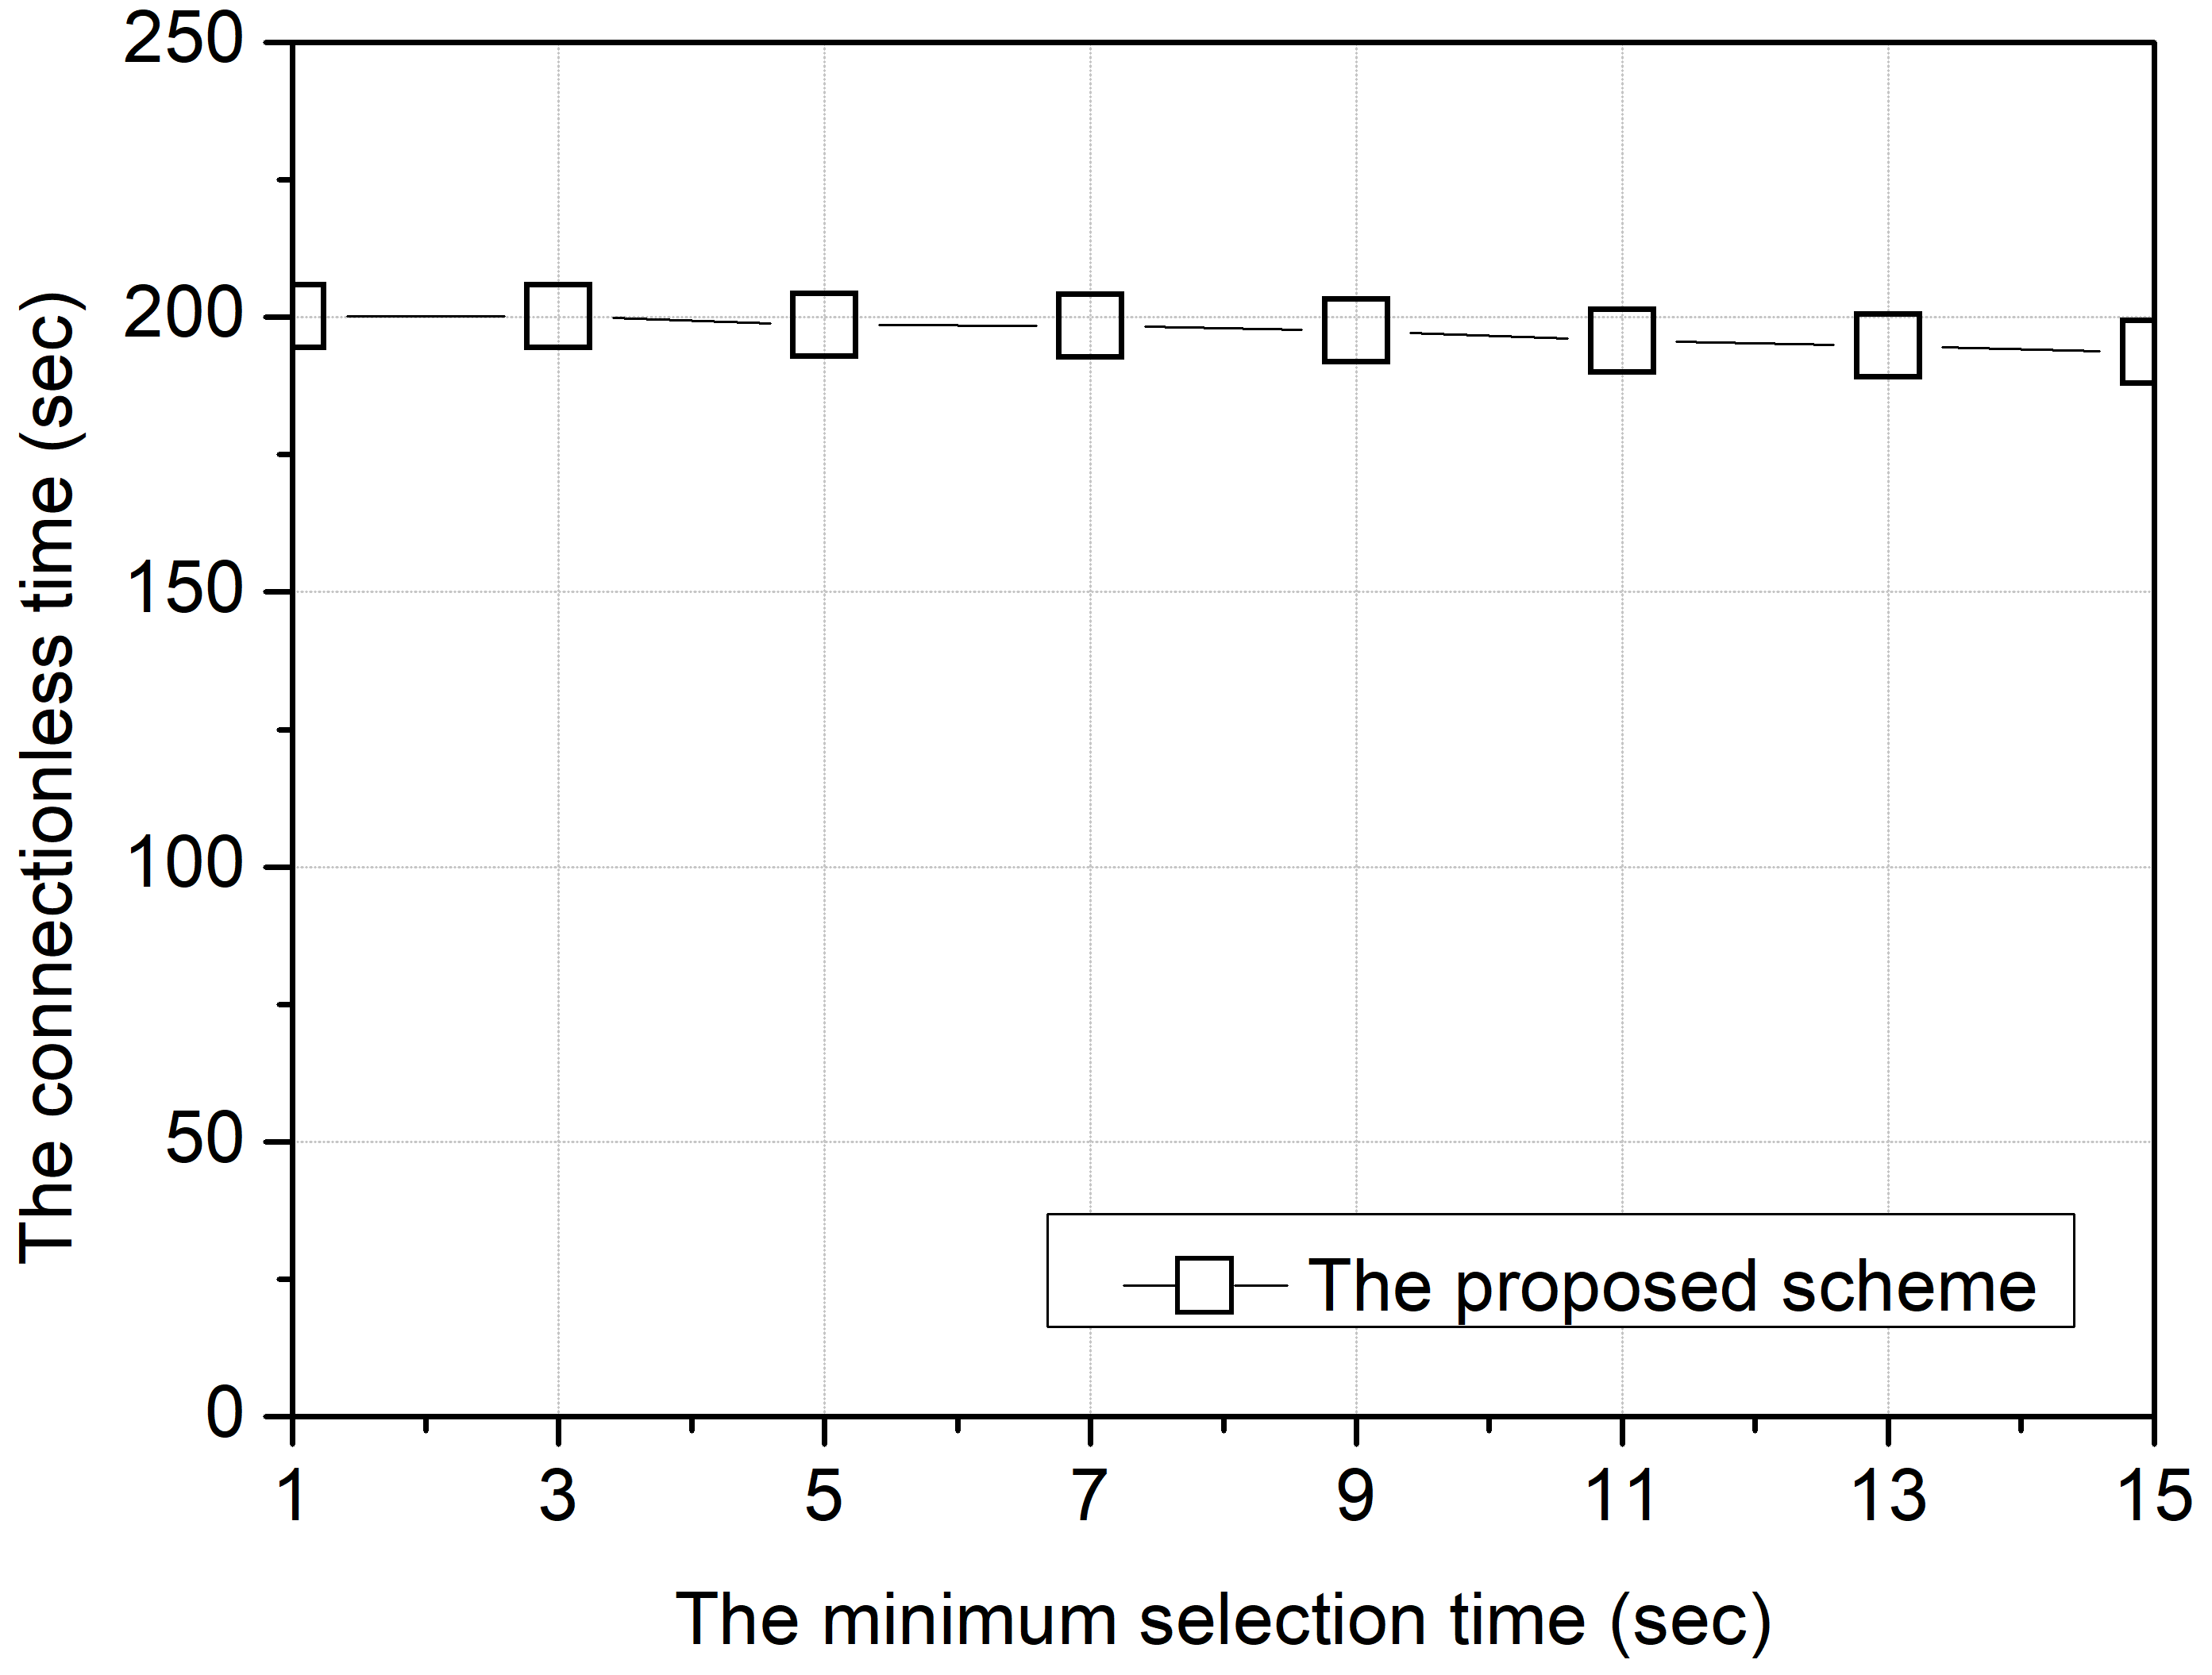
\includegraphics[width=.7\linewidth]{./graphs/IC.png}
    \caption{The connectionless time for the minimum selection~time.}
    \label{fig:int}
\end{figure}
\unskip

\begin{figure}[H]
     
    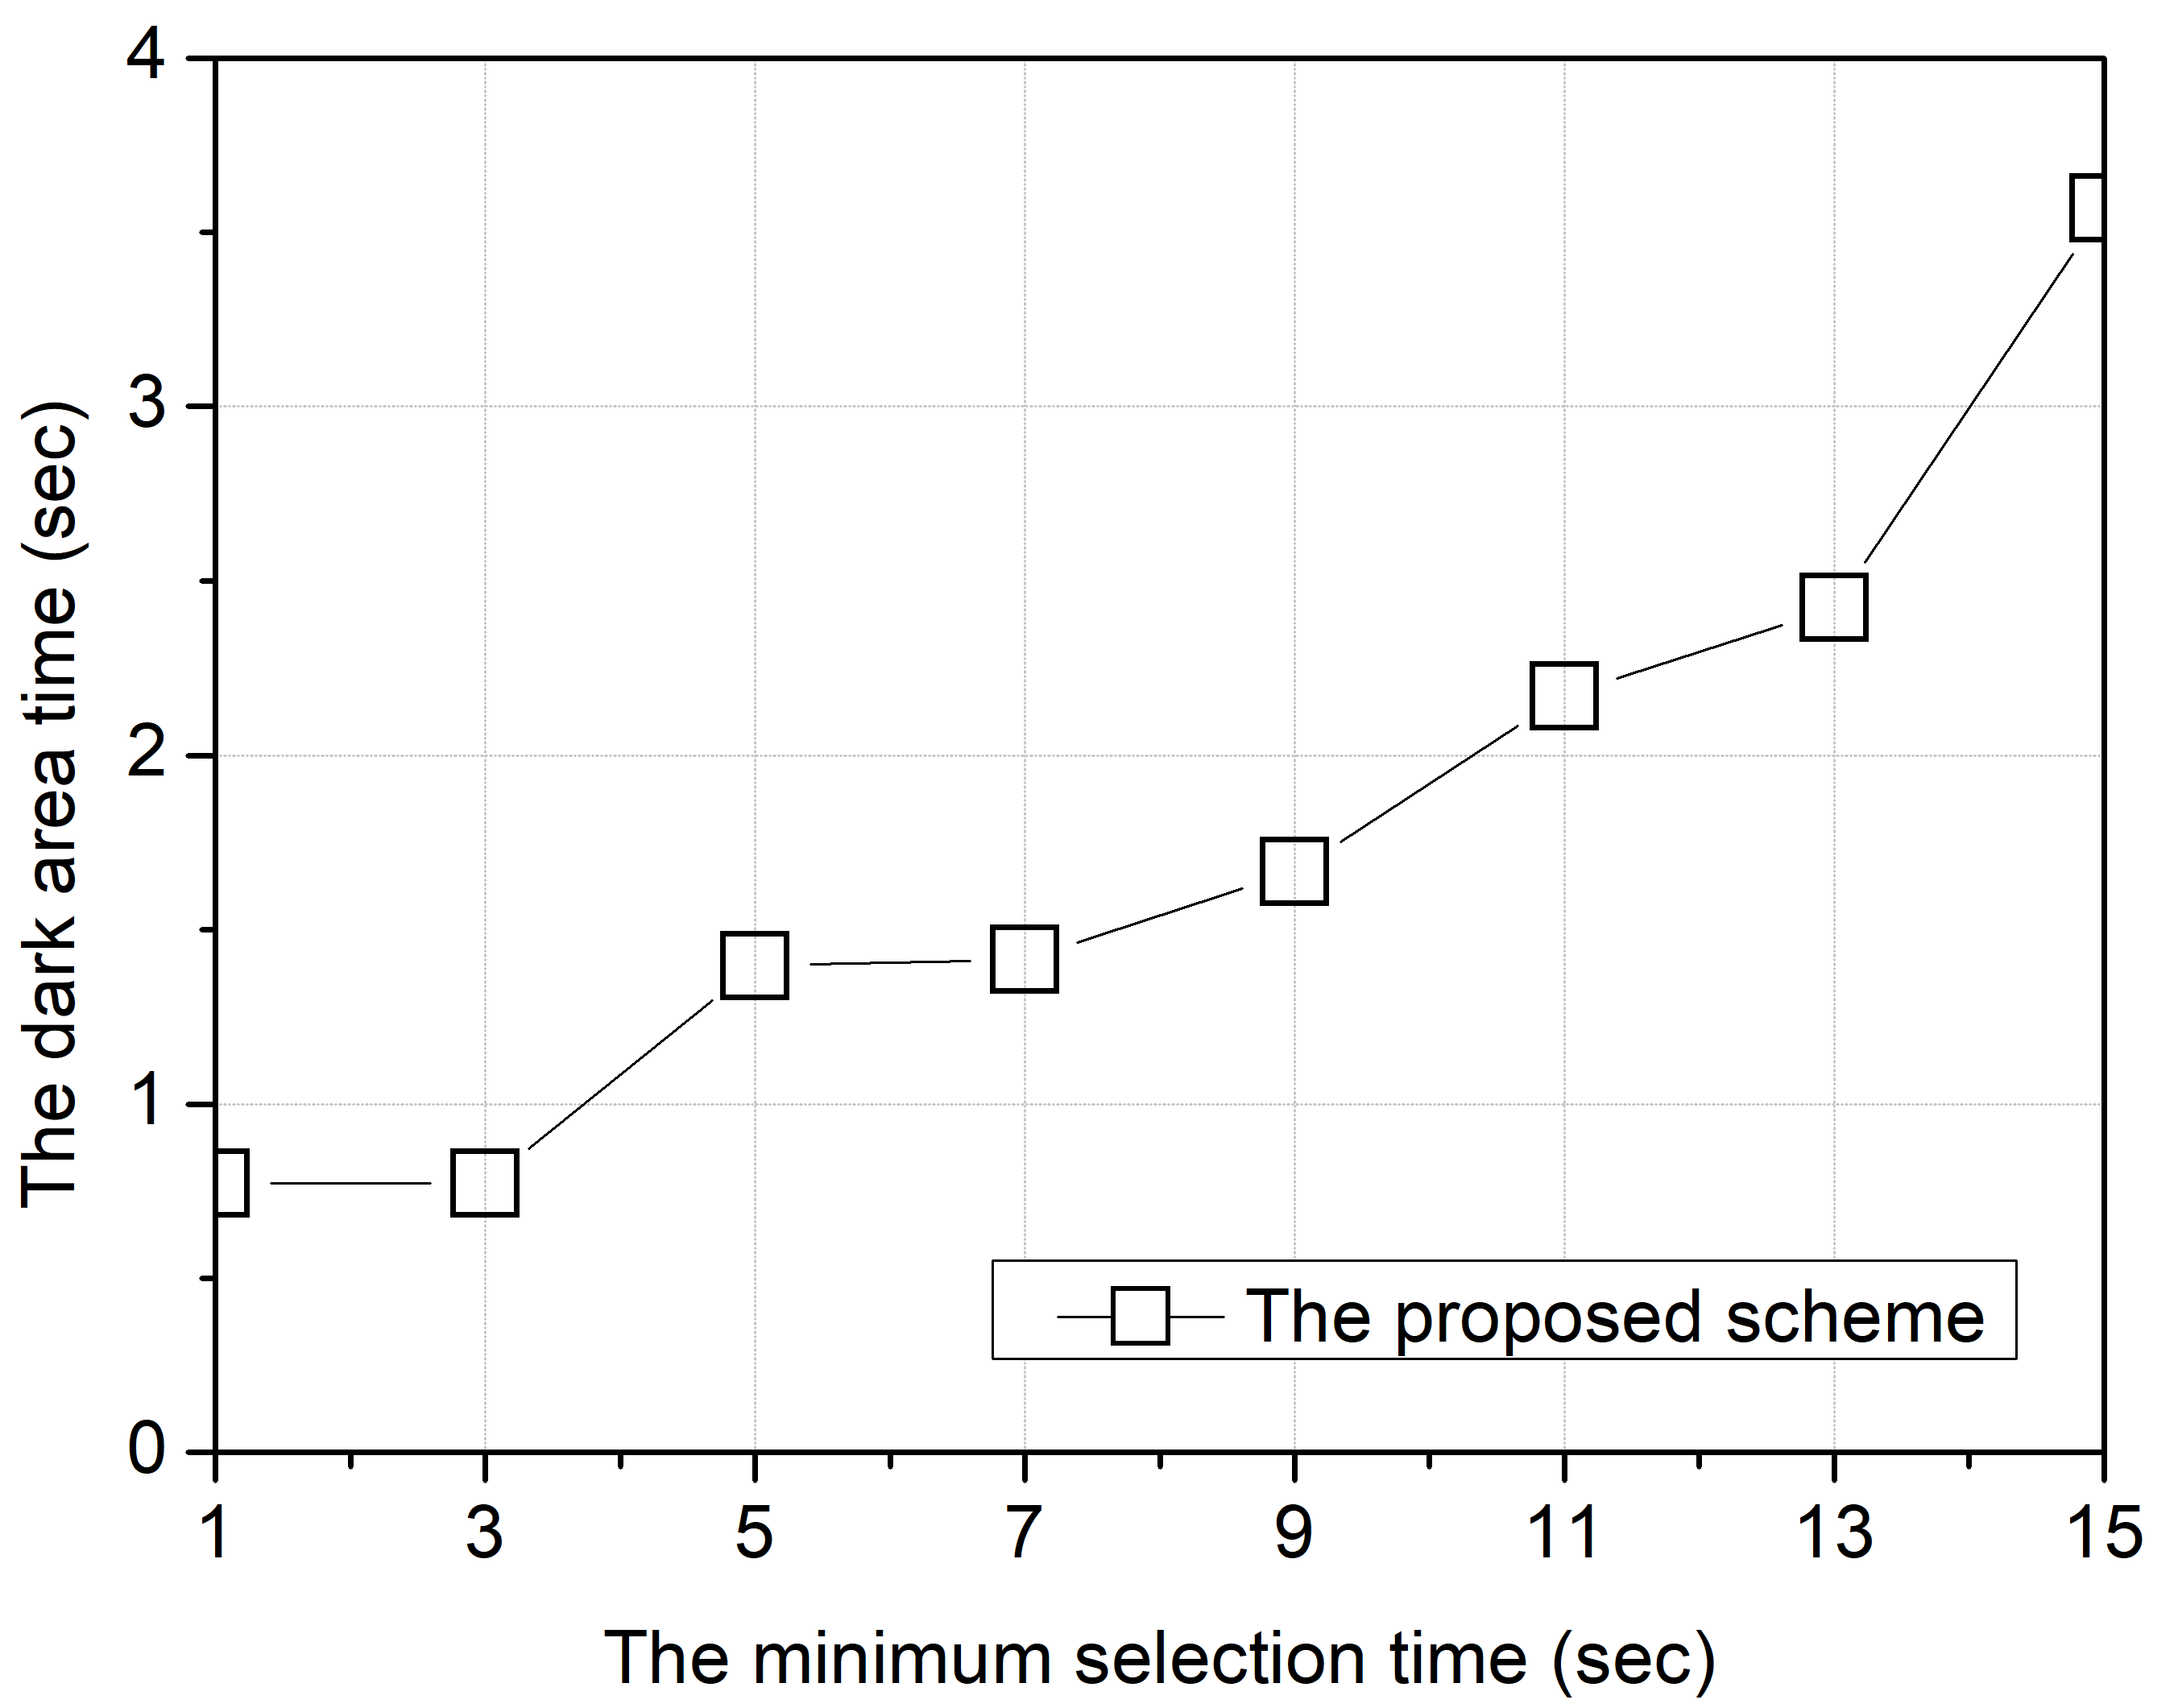
\includegraphics[width=.7\linewidth]{./graphs/ID.png}
    \caption{The dark area time for the minimum selection~time.}
    \label{fig:int2}
\end{figure}
\unskip


\subsection{Multiple First-Hop Precaching Vehicle~Selection} \label{sec3.3}

The first-hop precaching vehicles are first selected because the first hop is the foundation of connection for the requester vehicle in multi-hop communication, as shown in Figure~\ref{fig4}.
Since the requester vehicle is served by multi-hop precaching vehicles, the~selection of the first-hop precaching vehicle is more likely to focus on the connection time to the requester vehicle.
However, as~the requester vehicle has to access RSUs to download content within their coverage area because they have sufficient communication resources in the content provision services, the~connection time between the requester vehicle and a precaching vehicle must be considered based on the connectionless time within the outage zone.
To obtain the connectionless time, the~RSU has to calculate two times: the leave time from the current RSU of the requester vehicle, and the entrance time to the next RSU of the requester vehicle.
The RSU can determine the leave time based on $t_{dwell,j,req}$.
Then, it can calculate the entrance time $t_{enter,j+1,req}$ to the next RSU $R_{j+1}$ of $V_{req}$ as follows:







\begin{equation}
    t_{enter,j+1,req} = \cfrac{(x_{j+1} - Range_{j+1} - x_{req})}{v_{req}}.
\end{equation}

Based on $t_{enter,j+1,req}$ and $t_{out, j,req}$, the~RSU selects a first-hop precaching vehicle as shown in Figure~\ref{fig4}.
Then, the~RSU can obtain the meet time and leave time between the requester vehicle and a first-hop precaching vehicle.
For example, when representing two vehicles as $V_{a}$ and $V_{b}$, we can obtain the meet time $t_{m}(a,b)$ and the leave time $t_{l}(a,b)$, respectively, as follows:
\begin{equation}
    t_{m}(a,b)=\cfrac{x_{b}-x_{a}+Range_{a}}{v_{a}-v_{b}},
\end{equation}
and
\begin{equation}
    t_{l}(a,b)=\cfrac{x_{b}-x_{a}-Range_{a}}{v_{a}-v_{b}},
\end{equation}
where $x_{a}$ and $x_{b}$ are the location of the two vehicles; $v_{a}$ and $v_{b}$ represent the velocity of them; and $Range_{a}$ is the communication range of $V_{a}$.

In the same way, the~RSU can calculate the meet time and leave time between $V_{req}$ and a candidate vehicle for the $i$-th precaching vehicle $V_{i}$ within the outage zone using $t_{dwell,j,req}$ and $t_{enter,j+1,req}$, respectively, as follows:
\begin{equation}
    t_{meet,req,i}(t_{dwell,j,req}, t_{enter,j+1,req}) = \begin{cases}
        t_{dwell,j,req} & \text{if } \begin{split}
                                        t_{m}(req,i) < t_{dwell,j,req} \\
                                        t_{l}(req,i) < t_{dwell,j,req}
                                    \end{split}\\
        t_{enter,j+1,req} & \text{if } \begin{split}
                                        t_{m}(req,i) > t_{dwell,j,req} \\
                                        t_{l}(req,i) > t_{dwell,j,req}
                                    \end{split}\\
        t_{m}(req,i) & \text{if } t_{m}(req,i) < t_{l}(req,i)\\
        t_{l}(req,i) & \text{else,}
    \end{cases}
\end{equation}
and
\begin{equation}
    t_{leave,req,i}(t_{dwell,j,req}, t_{enter,j+1,req}) = \begin{cases}
        t_{dwell,j,req} & \text{if } \begin{split}
                                        t_{m}(req,i) < t_{dwell,j,req} \\
                                        t_{l}(req,i) < t_{dwell,j,req}
                                    \end{split}\\
        t_{enter,j+1,req} & \text{if } \begin{split}
                                        t_{m}(req,i) > t_{dwell,j,req} \\
                                        t_{l}(req,i) > t_{dwell,j,req}
                                    \end{split}\\
        t_{m}(req,i) & \text{if } t_{m}(req,i) > t_{l}(req,i)\\
        t_{l}(req,i) & \text{else.}
    \end{cases}
\end{equation}


With the two calculated times, the~RSU can obtain the connection time $t_{conn,req,i}$ with $t_{dwell,j,req}$ and $t_{enter,j+1,req}$ between $V_{req}$ and $V_{i}$ within the outage zone as follows:
\begin{equation}
    \begin{split}
        t_{conn,req,i}(t_{dwell,j,req}, t_{enter,j+1,req}) = & t_{leave,req,i}(t_{dwell,j,req}, t_{enter,j+1,req}) \\
                        & - t_{meet,req,i}(t_{dwell,j,req}, t_{enter,j+1,req}).
    \end{split}
\end{equation}

Based on the $t_{conn,req,i}$ of every $V_{i}$, the $V_{i}$ with the biggest connection time is selected as the first-hop precaching vehicle $V_{1.1}$ and its available amount $C_{avail,req,1.1}$ of content is calculated as follows:
\begin{equation}
    C_{avail,req,1.1} = t_{conn,req,1.1} \times r_{1.1},
\end{equation}
where $r_{1.1}$ is the transmission rate of $V_{1.1}$.
When $C_{need,req}$ is smaller than $C_{avail,req,1.1}$, $R_{j}$ finishes the selection process.
Otherwise, it keeps selecting another first-hop precaching vehicle.
The RSU compares the connectionless times before and after the connecting of $V_{req}$ and $V_{i}$ with $t_{ms}$, respectively.
The connectionless time can be divided into before and after based on the connection time with $V_{1.1}$.
Then, the~RSU checks whether more precaching vehicles are needed to cover the outage zone by comparing $t_{ms}$ and the two connectionless times.
If the connectionless time is longer than $t_{ms}$, the~RSU searches for more precaching vehicles to cover the outage zone.
Until all connectionless times are shorter than $t_{ms}$, $R_{j}$ searches more first-hop $k$-th precaching vehicles within the connectionless area based on the biggest connection time $t_{conn,req,i}(t_{leave, req, 1.(k-1)}, t_{meet, req, 1.k+1})$, where $t_{leave, req, 1.(k-1)}$ denotes the disconnect time between $V_{req}$ and $V_{1.(k-1)}$, and $t_{meet, req, 1.k+1}$ denotes the meeting time between $V_{req}$ and $V_{1,k+1}$.
After selecting the new precaching vehicle, $R_{j}$ reorders the number of precaching vehicles in the order in which they meet $V_{req}$.
When $C_{need,req} \leq \sum^{K}_{k=1}{C_{avail,req,1.k}}$ and all connectionless times are shorter than $t_{ms}$, $R_{j}$ stops finding other first-hop precaching~vehicles.


\begin{figure}[H]
    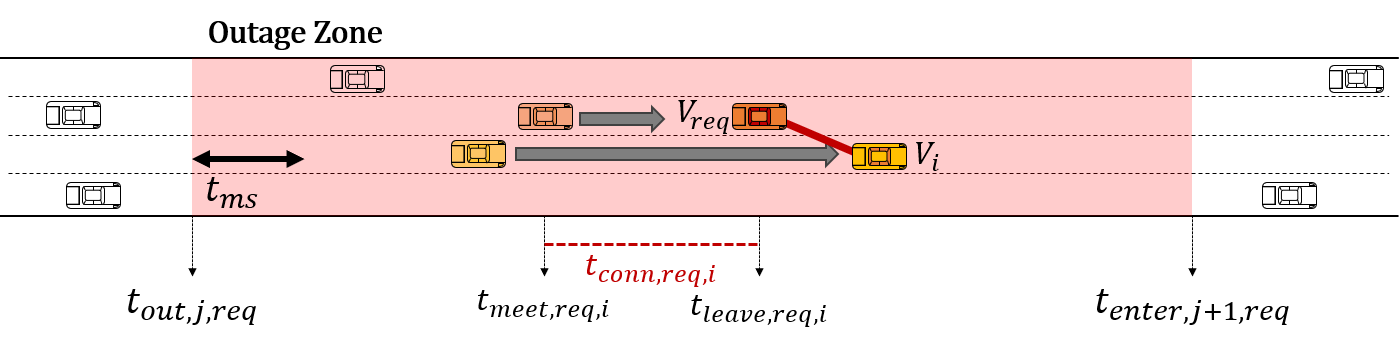
\includegraphics[width=\textwidth]{./figures/1hop.png}
    \caption{The process of first-hop precaching vehicle~selection.}
    \label{fig4}
\end{figure}




\subsection{Multiple Second-Hop Precaching Vehicle~Selection} \label{sec3.4}

The RSU has to search the second-hop precaching vehicles when the first-hop precaching vehicles have too long a connection time to $V_{req}$ by comparing this time with the time required to deliver the content, as shown in Figure~\ref{fig5}.
Since a first-hop precaching vehicle $V_{1.k}$ has a limited time to deliver the content due to the dwell time of $V_{req}$, it cannot deliver all parts of its $C_{avail,req,1.k}$.
Also, when $V_{1.k}$ has a shorter time to deliver than the connection time to $V_{req}$, it cannot deliver more content to $V_{req}$ in the outage zone.
Therefore, the~RSU should know the precaching time $t_{prec,1.k}$ of $V_{1.k}$ and $t_{prec,1.k}$, which can be determined as follows:
\begin{equation}
    t_{prec,1.k} =  \begin{cases}
                        t_{dwell, j, 1.k} & \text{if }t_{dwell,j,1.k} < t_{dwell,j,req} \\
                        t_{dwell,j,req} & \text{else.}
                    \end{cases}
\end{equation}
Based on $t_{prec,1.k}$, the~RSU can define the precaching amount $C_{prec,1.k}$ of $V_{1.k}$ as follows:
\begin{equation}
    C_{prec,1.k}=t_{prec,1.k}\times r_{j}.
\end{equation}

In this second-hop precaching vehicle selection, the~RSU has to consider $t_{ms}$.
If $t_{conn,req,1.1} - t_{prec,1.k}$ is longer than $t_{ms}$ within the outage zone, $V_{1.k}$ needs to connect second-hop precaching vehicles within its connection time after it delivers all of its precached content to $V_{req}$ in the outage zone.
Then, a~second-hop precaching vehicle has to deliver its precached content after $V_{1.k}$ delivers $C_{prec,1.k}$.
Therefore, the~RSU has to define the end time $t_{end,1.k}$ to precache $V_{1.k}$'s $C_{prec,1.k}$ as follows:
\begin{equation}
    t_{end,1.k} = t_{meet,req,1.k} + \cfrac{C_{prec,1.k}}{r_{1.k}},
\end{equation}
\textls[-15]{where $r_{1.k}$ is the transmission rate of $V_{1.k}$.
Based on $t_{end,1.k}$ and $t_{leave,req,i}(t_{dwell,j,req}, t_{enter,j+1,req})$,} the~RSU can select the second-hop precaching vehicle from the time when $V_{1.k}$ finishes delivering its precached content to $V_{req}$ to the time when $V_{1.k}$ and $V_{req}$ are disconnected by communication range limitation, as shown in Figure~\ref{fig5}.
The connection time of the second-hop candidate vehicle is denoted by $t_{conn,req,2^{k}.1}(t_{ end ,1.k}, t_{leave,req,1.k})$.
Then, the~candidate vehicle with the maximum connection time becomes the second-hop precaching vehicle within the connection time between $V_{req}$ and $V_{1.k}$, which is denoted as $V_{2^{k},1}$.
Then, the~connection time of the second-hop $l$-th precaching vehicle must be inside the period between $t_{leave,req,2^{k}.(l-1)}$ and $t_{meet,req,2^{k}.(l)}$.
Also, in~every selection of the second-hop precaching vehicles, the~RSU has to consider $t_{ms}$. 

After the selection of second-hop precaching vehicles, they precache the assigned amount of the content, which is $C_{prec,2^{k}.(l)}$.
Then, when the first-hop precaching vehicle finishes its precached content delivery in the outage zone and it has more time in which it is possible to deliver the content during its connection time within the outage zone, the~second-hop precaching vehicle delivers its precached content to the first-hop precaching vehicle.
The first-hop precaching vehicle delivers the content to $V_{req}$, as shown in Figure~\ref{fig5}.

\vspace{-5pt}
\begin{figure}[H]
    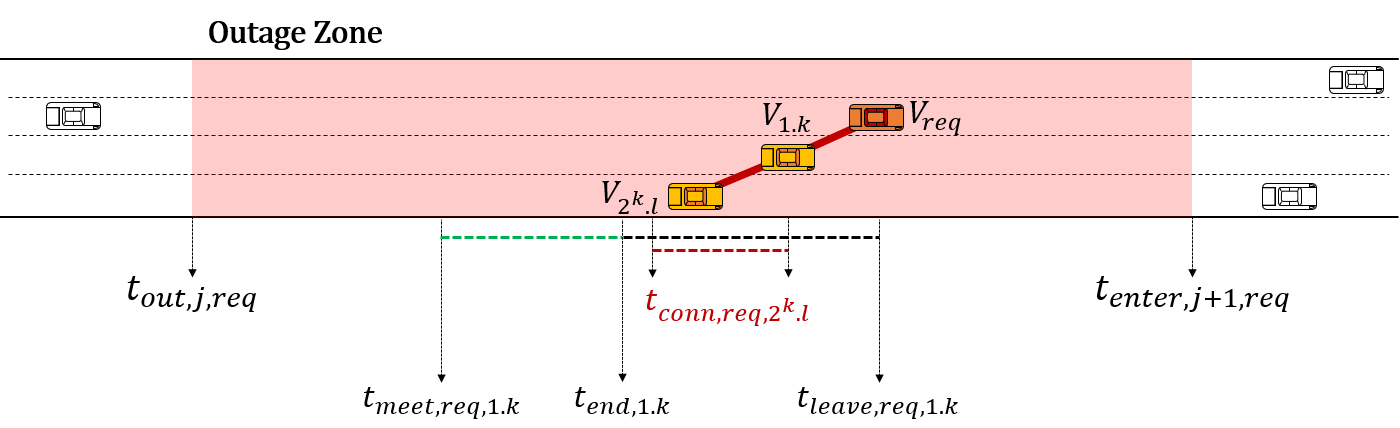
\includegraphics[width=\textwidth]{./figures/2hop.png}
    \caption{The process of second-hop precaching vehicle~selection.}
    \label{fig5}
\end{figure}


\subsection{Multiple Third-Hop Precaching Vehicle~Selection} \label{sec3.5}


In the proposed scheme, because~the second-hop precaching vehicles may have insufficient precaching time, as shown in Figure~\ref{fig6}, the~RSU needs to select third-hop precaching vehicles for the requester vehicle in the outage zone.
This is necessary to ensure that the requester vehicle $V_{req}$ receives the requested content without interruption during its journey through the outage zone.
The selection of third-hop precaching vehicles addresses the limitations of the second-hop precaching vehicles by providing additional precached content when the second-hop precaching vehicles cannot cover the entire duration required for content delivery.
In the selection of the third-hop precaching vehicle, the~RSU considers $t_{end,2^{k}.l}$ based on $t_{prec,2^{k}.l}$.
Then, using $t_{leave,1.k,2^{k}.l}$, the~RSU can define the dark area time of $V_{2^{k}.l}$.
If the dark area time is longer than $t_{ms}$, it searches third-hop precaching vehicles.
It is necessary to consider the connection time of the vehicles with $V_{2^{k}.l}$ within the range between $t_{end,2^{k}.l}$ and $t_{leave,1.k,2^{k}.l}$ to guarantee the effective precaching of content. 
This range ensures that the third-hop precaching vehicles can connect to $V_{2^{k}.l}$ right after $V_{2^{k}.l}$ finishes its content transmission and before it loses connection with $V_{1.k}$.
Consequently, it guarantees that the third-hop precaching vehicle can continue the content transmission without interruption, maintaining the integrity and continuity of the content precaching~process.





After the third-hop precaching vehicle precaches all of its precached content, it cannot be helped by other vehicles.
Therefore, the~RSU should consider its precaching time in this third-hop precaching vehicle selection.
Thus, the~available amount of $C_{avail,req,3^{k,l}.m}$ of a third-hop $m$-th precaching vehicle $V_{3^{kl}.m}$ is denoted as follows:

\begin{equation}
    C_{avail,req,3^{k,l}.m}=\begin{cases}
        t_{conn,req,3^{k,l}.m}\times r_{3^{k,l}.m} & 
                \text{if }t_{conn,req,3^{k,l}.m} < t_{prec,3^{k,l}.m}\\
        t_{prec,3^{k,l}.m}\times r_{3^{k,l}.m} & 
                \text{else.}
    \end{cases}
\end{equation}

The RSU selects the vehicle with the biggest $C_{avail,req,3^{k,l}.m}$ as the third-hop precaching vehicle between $t_{end, 2^{k}.l}$ and $t_{leave, 1.k, 2^{k}.l}$, as shown in Figure~\ref{fig6}.
The connection time of $V_{3^{kl}.m}$ must be inside the period between $t_{leave,2^{k}.l,3^{(k-1),l}.m}$ and $t_{meet,2^{k}.l,3^{(k+1),l}.m}$.
This selection also is conducted based on $t_{ms}$.

All precaching vehicles download their assigned parts of content from the RSU until $V_{req}$ leaves the RSU.
When the first-hop precaching vehicle meets $V_{req}$, it delivers its precached content to $V_{req}$ in the outage zone.
During the remaining connection time after providing all its precached content, the~second-hop precaching vehicle delivers its precached content to the first-hop precaching vehicle when they meet.
Then, the~first-hop precaching vehicle precaches that content to $V_{req}$.
If the second-hop precaching vehicle is still connected to the first-hop precaching vehicle after delivering all its precached content, the~third-hop precaching vehicle delivers its precached content to the second-hop precaching vehicle when they meet.
The second-hop precaching vehicle precaches the content to the first-hop precaching vehicle and the first-hop precaching vehicle precaches the content to $V_{req}$, as shown in Figure~\ref{fig6}.

The RSU first selects the first-hop precaching vehicles, as~shown in Algorithm \ref{algo.2}.
If the available number of them is enough, the~RSU finishes this process.
Otherwise, the~RSU selects the second-hop precaching vehicles based on the first-hop precaching vehicles.
Every time a second-hop precaching vehicle for each first-hop precaching vehicle is selected, the~RSU checks the available number of them.
If there are not enough second-hop precaching vehicles, the~RSU selects the third-hop precaching vehicles based on previous-hop precaching vehicles.
In this selection, the~RSU also checks the available number of the selected vehicles as a precaching vehicle in every~selection.

The multiple precaching vehicle selection is conducted within the given range, as~shown in Algorithm \ref{algo.1}.
In the case of first-hop precaching vehicle selection, the~given range is the connectionless time between $t_{out, j,req}$ and $t_{enter,j+1,req}$.
Based on the algorithm, the~RSU first checks that the connectionless time is longer than $t_{ms}$.
Then, except~the third-hop precaching vehicle selection, the~RSU selects the vehicle with the longest connection time with $V_{req}$.
In the third-hop precaching vehicle selection, the~RSU considers the available number of candidate vehicles.
If the selected vehicle can resolve the requested size of the content from $V_{req}$, the~RSU finishes this process.
Otherwise, the~RSU selects more relaying vehicles by comparing the rest time to $t_{ms}$.
Since the early-connected precaching vehicle has a higher priority than the later-connected precaching vehicle, $V_{select}[Left]$ is selected before $V_{select}[Right]$.

\vspace{-5pt}
\begin{figure}[H]
    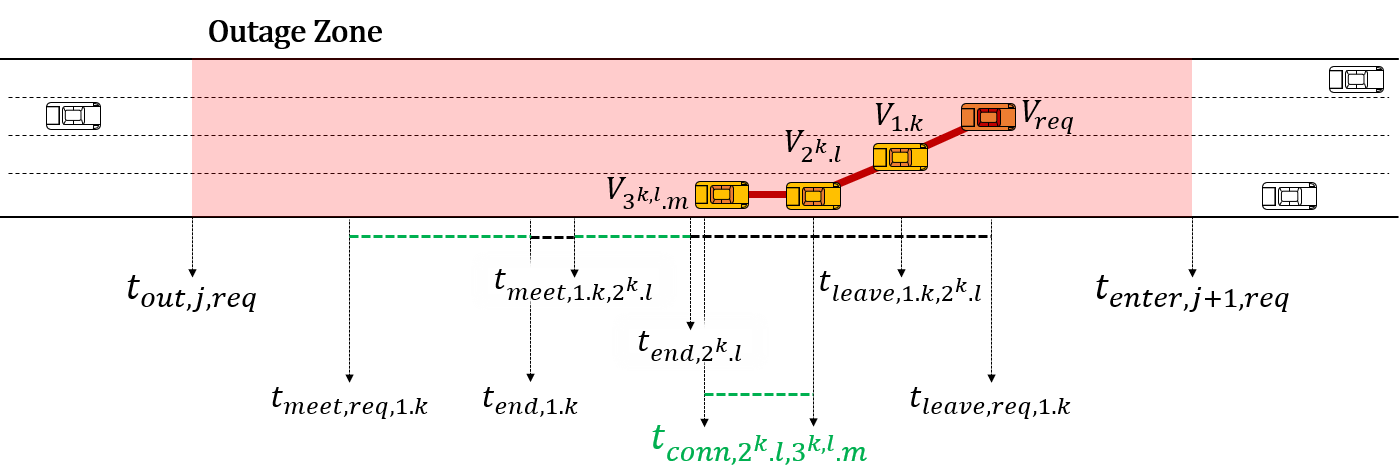
\includegraphics[width=\textwidth]{./figures/3hop.png}
    \caption{The process of third-hop precaching vehicle~selection.}
    \label{fig6}
\end{figure}


\section{Performance~Evaluation} \label{sec4}
In this section, we evaluate the performance of the proposed scheme through simulations. First, we describe the simulation environment and the performance evaluation metrics used. Next, we compare the performance of the proposed scheme with that of existing schemes based on the simulation~results.

\subsection{Simulation Environments and Performance Evaluation~Metrics}



For the performance evaluation of the proposed scheme, we conducted simulations using Network Simulator 3 (NS3)~\cite{NS3}. We implemented an enhanced Manhattan mobility model to reflect an urban environment suitable for CCVNs.
Table~\ref{table2} shows the simulation parameters used in our simulations.
We focus on how much of the outage zone can be covered according to the physical properties of the vehicle and the RSU. We evaluated the proposed scheme in a road environment where RSUs are located 8 km away and the density of the vehicles is 100 per {km}$^{2}$. We used Gaussian distribution to create a road situation in which vehicles move at a constant speed with an error range of 10$\%$ at each average speed. 
The average speed is 40 km/h, and~vehicles on the road have speeds between 20 km/h and 120 km/h depending on the Gaussian distribution.
Among these vehicles, the~vehicles within the communication range of an RSU send their location and speed information to the RSU using beacon messages.
All entities, including RSUs and vehicles, communicate using 802.11p WAVE and have a maximum transmission rate of 54 Mbps. RSUs and vehicles have a maximum communication range of 800 and 200 meters, respectively. Since RSUs are deployed every 8 km, the~outage zone is 6.4 km. The~requester vehicle requests 2000~MB of content in such a road environment. The~\textit{minimum selection time} is set to 3 s. If~the connectionless time or the dark area time exceeds 3 s, the~precaching vehicle is selected in the proposed~scheme.


\begin{table}[H] % Table~2
    \caption{Simulation environment~parameters.}
    
    \begin{tabularx}{\textwidth}{LL}
        \toprule
        \textbf{Parameters} & \textbf{Value} \\
        \midrule 
        The radio channel rate & 6 Mbps\\
        The distance between RSUs & 8 km\\
        The outage zone & 6.4 km\\
        The vehicle density & 100 per {km}$^{2}$\\
        The request size of the content & 2000 MB\\
        The vehicle speed & [20, 120] km/h\\
        The V2I communication range & 800 m\\
        The V2V communication range & 200 m\\
        
        % %%%%%%%%%%%%% Revision on 2024.08.14. %%%%%%%%%%%%%%%%%%%
        The storage limit of a vehicle & 512 GB\\
        The storage limit of an RSU & 1 TB\\
        The amount of content & 1,000,000\\
        %%%%%%%%%%%%%%%%%%%%%%%%%%%%%%%%%%%%%%%%%%%%%%%%%%%%%%%%%%%
        
        The prediction error & [0,1]\\
        The minimum selection time & 3 s\\
        \bottomrule
    \end{tabularx}
    \label{table2}
\end{table}




We evaluated the performance of the proposed scheme by comparing it with two existing schemes, the Adaptive Carry--Store--Forward (ACSF) scheme~\cite{Wu2013} and the Set Ranking-based Precaching (SRP) scheme~\cite{Nam2023}, both of which rely on single-hop communication for selecting precaching vehicles.
ACSF uses only one precaching vehicle moving in the same direction as the requester vehicle. In~ACSF, when a requester vehicle reaches the midpoint of an RSU’s communication range, vehicles driving in the same direction behind the requester vehicle become candidates for precaching. The~RSU calculates the time when these candidate vehicles are connected to both the RSU and the requester vehicle. Based on these calculations, only the vehicle that can deliver the most content to the requester vehicle is selected as the precaching vehicle for the outage zone.
On the other hand, SRP efficiently selects multiple vehicles for precaching to deliver more content in outage zones. SRP identifies sets of vehicles capable of successful content precaching by calculating download and delivery times and content amounts based on the vehicles' mobility information. It then ranks each set according to the number of vehicles and their available resources. Finally, SRP selects the highest-ranked set and utilizes those vehicles as precaching vehicles for content delivery in the outage~zone.

As performance evaluation metrics, we measured the connectionless time and dark area time under various simulation conditions. Connectionless time refers to the period when the requester vehicle remains in the outage zone without being connected to any precaching vehicle. Dark area time refers to the time during which the requester vehicle is connected to a precaching vehicle but cannot receive any content because the precaching vehicle has no more content to~deliver.

\subsection{Simulation~Results}



Figure~\ref{fig:my_label}a shows the dark area time relative to vehicle density. As~vehicle density increases, more candidate vehicles become available, which reduces the dark area time for all schemes. ACSF exhibits the highest dark area time across all densities. Although~dark area time decreases with higher vehicle density, it remains elevated because often, only one precaching vehicle is available, leading to insufficient content delivery. SRP reduces dark area time compared to ACSF by utilizing multiple precaching vehicles; however, since it operates within a single-hop range, there can still be instances of insufficient content during connection times. Overall, the~dark area time is lower than that of ACSF due to connections with other vehicles. The~proposed scheme demonstrates the lowest dark area time by employing multiple precaching vehicles in a multi-hop range, facilitating continuous content delivery from RSUs. As~vehicle density increases, dark area time further decreases, indicating the most efficient~performance.

\begin{figure}[H]
    \raggedright \subfloat[\centering \label{fig7:a}]{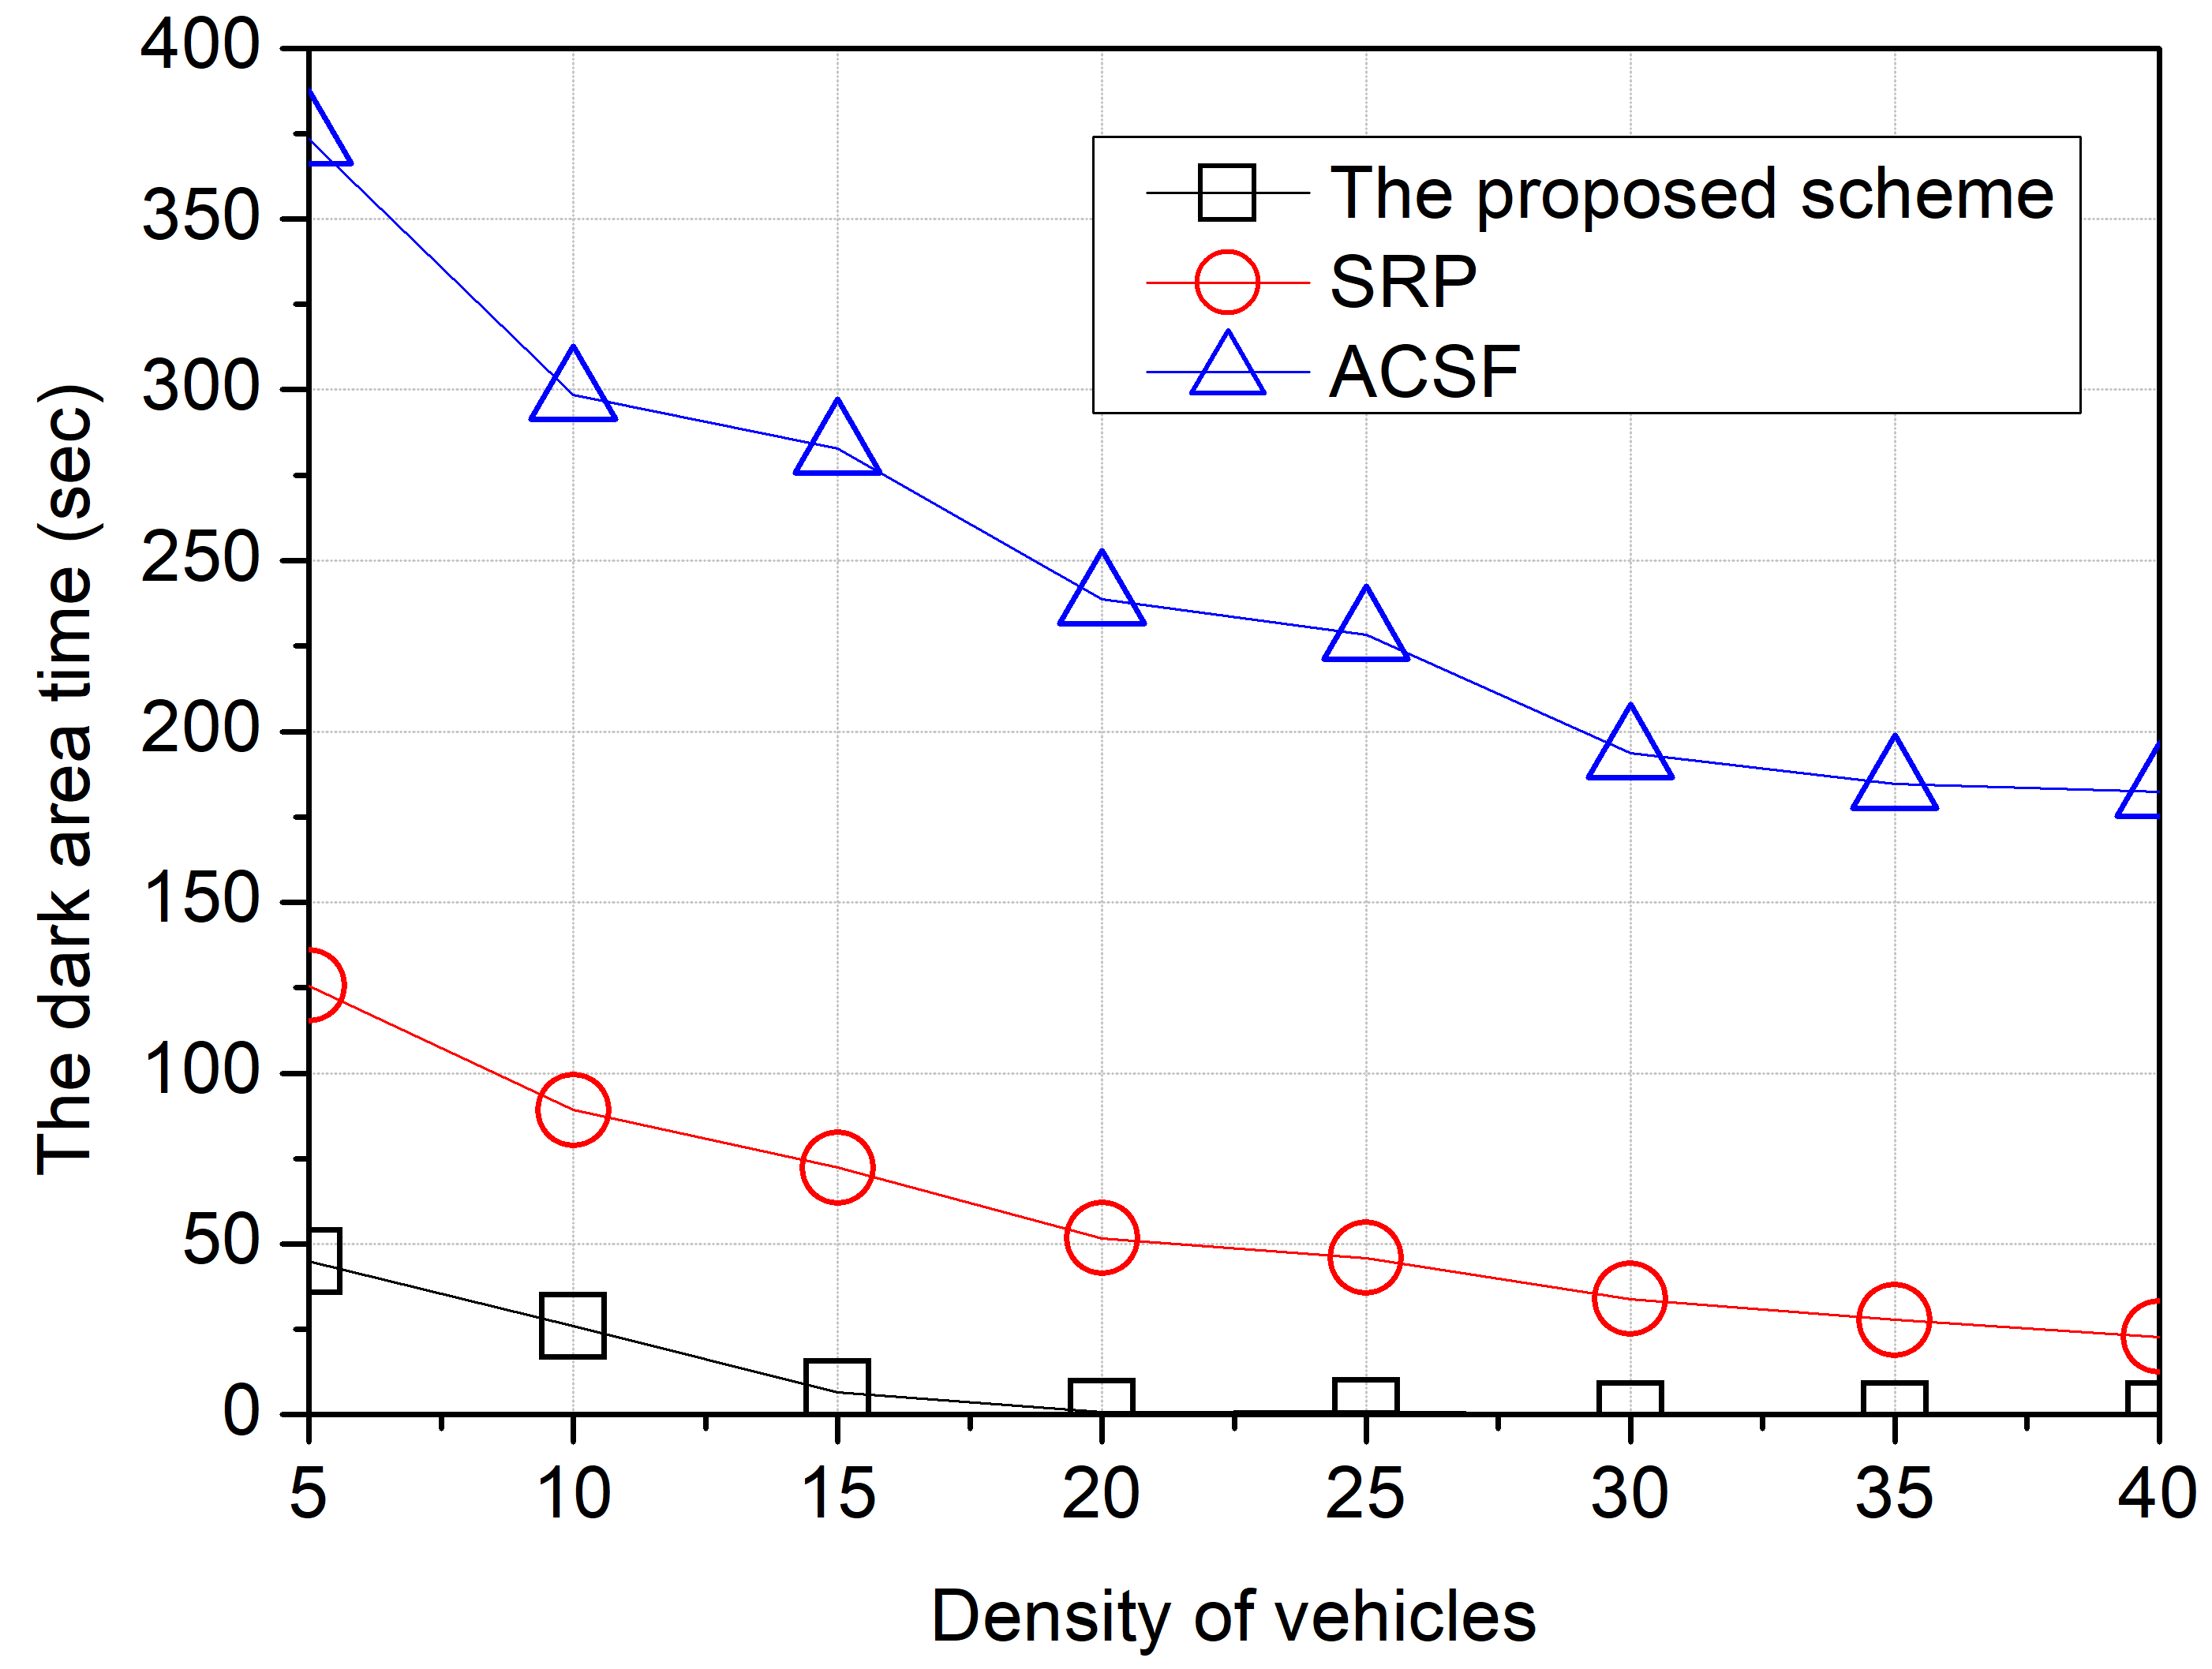
\includegraphics[width=.48\linewidth]{./graphs/DD.png}}
     \hspace{6pt}
    \raggedright \subfloat[\centering \label{fig7:b}]{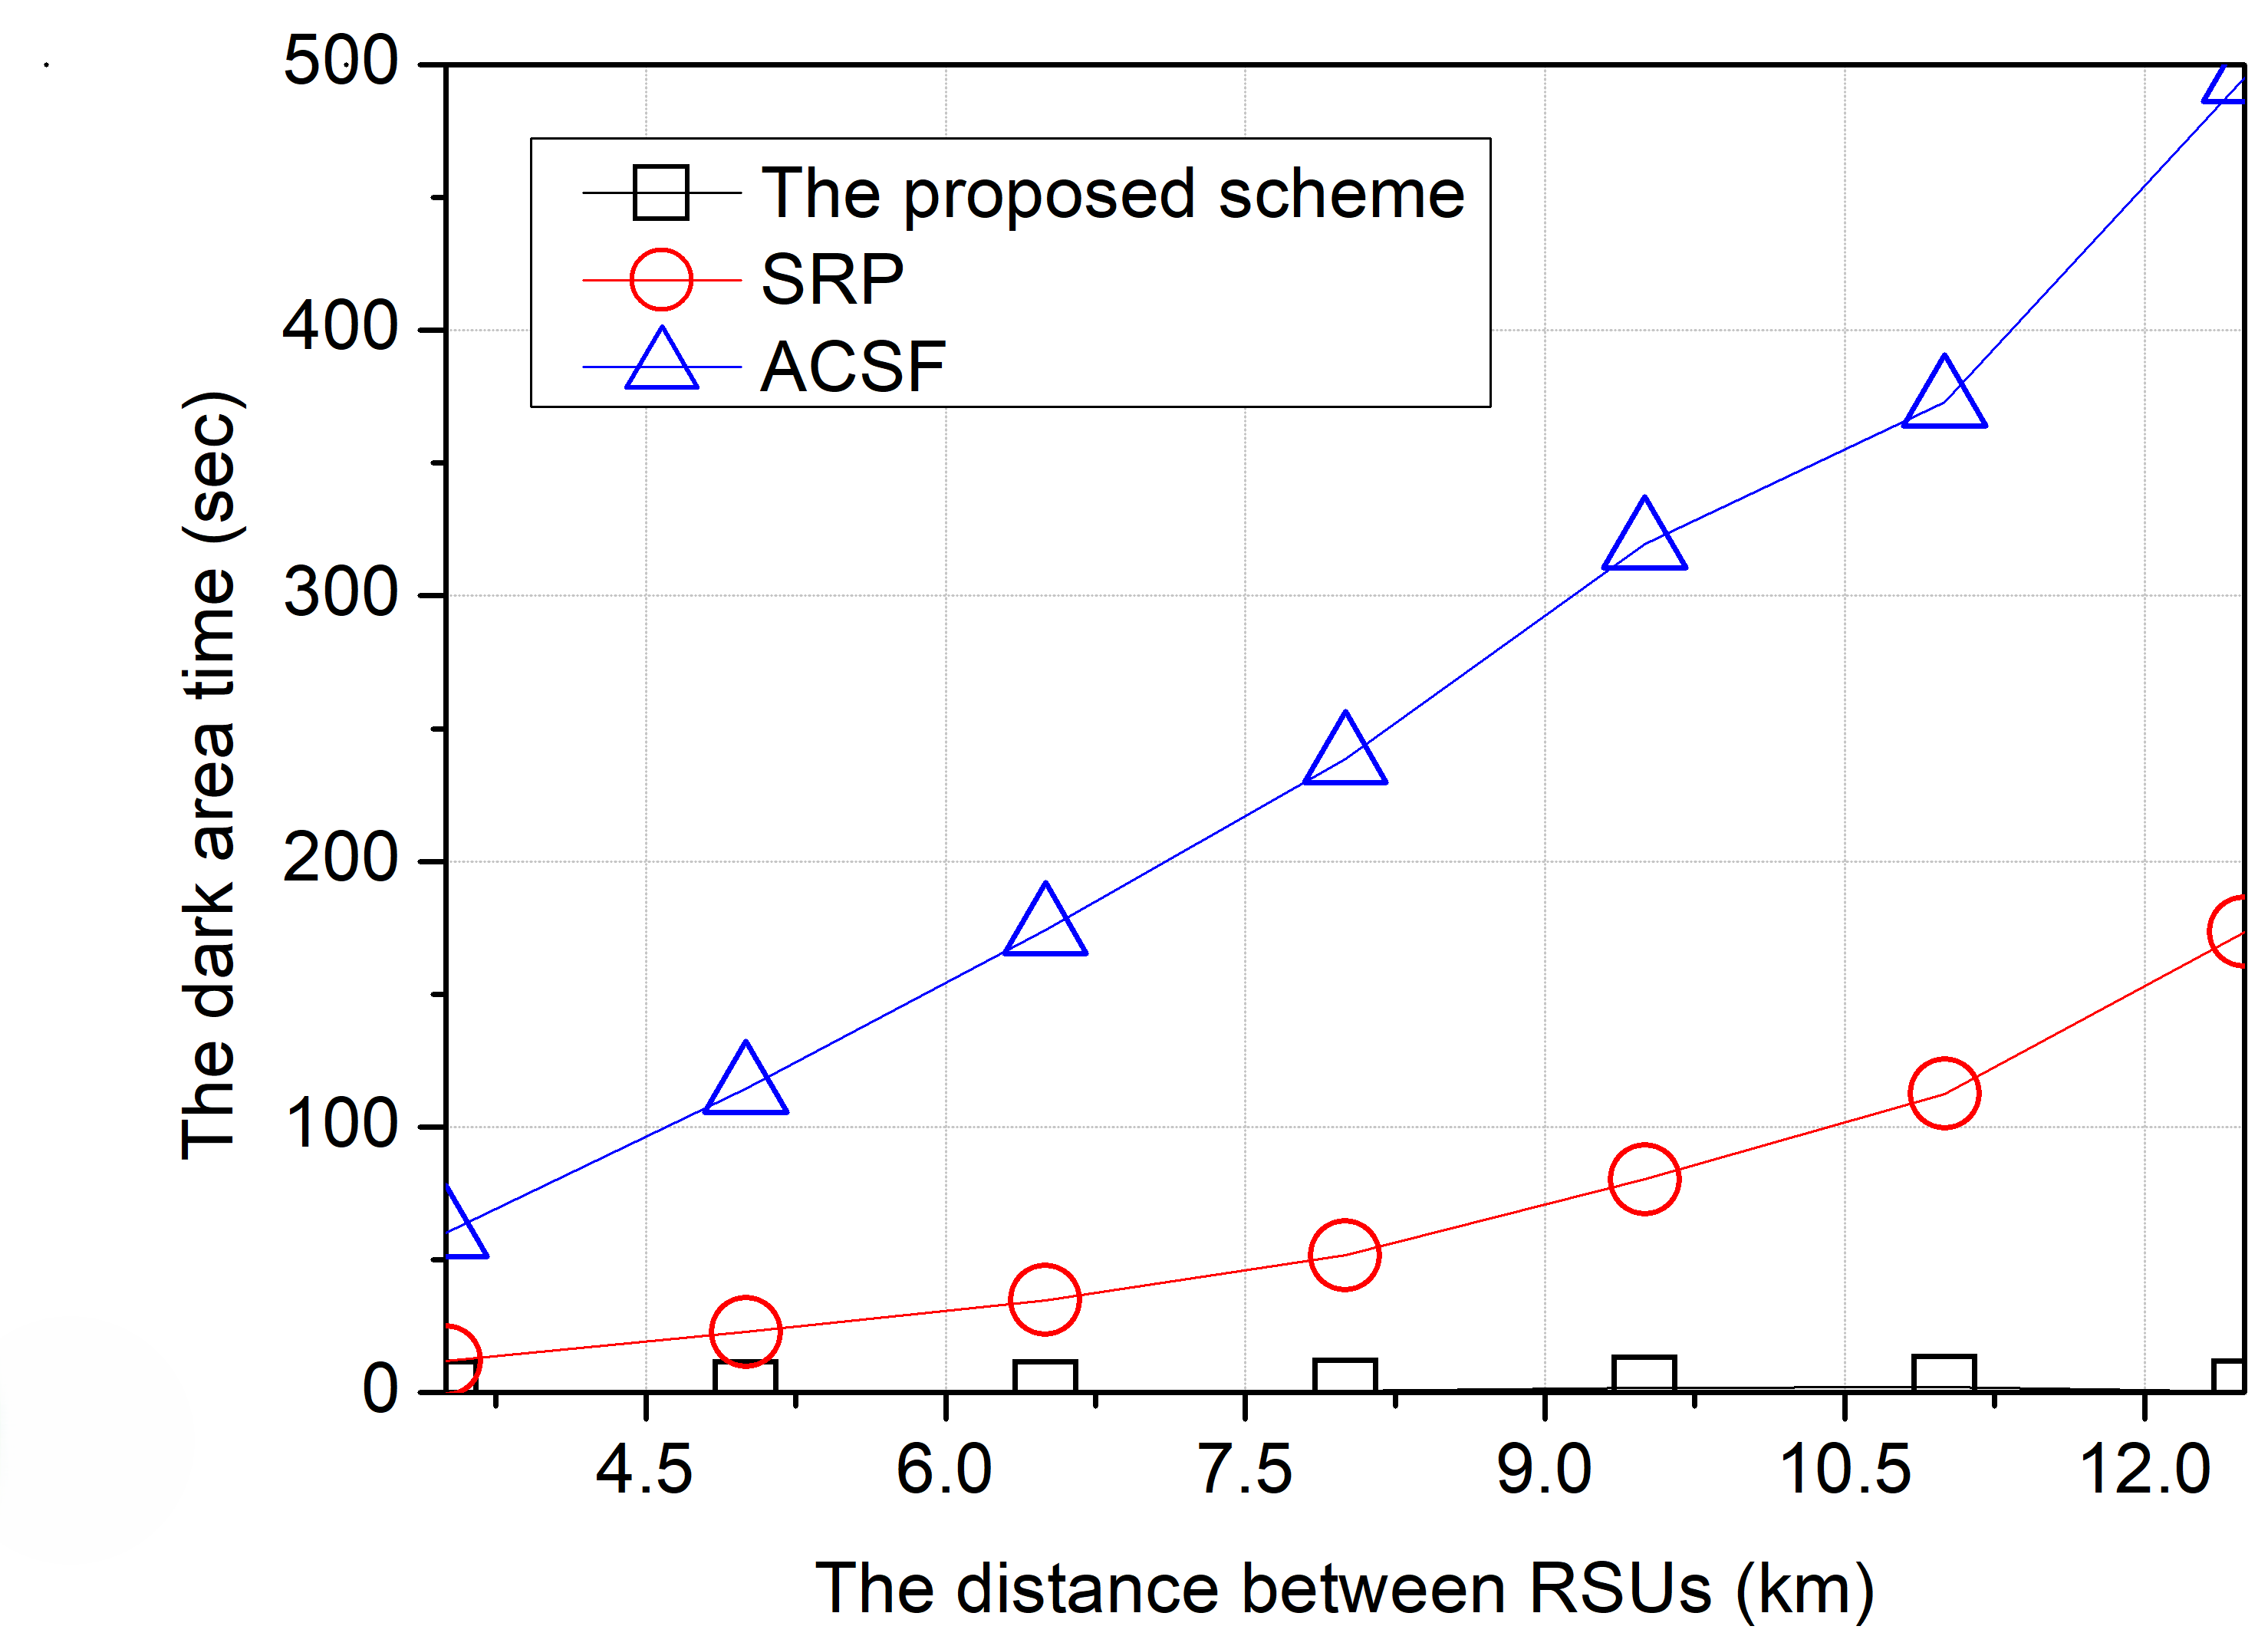
\includegraphics[width=.48\linewidth]{./graphs/LD.png}}
    \caption{The dark area time according to (\textbf{a}) the density of vehicles; (\textbf{b}) the distance between RSUs.}
    \label{fig:my_label}
\end{figure}

Figure~\ref{fig:my_label}b shows the dark area time relative to the distance between RSUs. As~the distance between RSUs increases, the dark area time also rises because vehicles spend more time in dark areas without receiving content. ACSF, which uses a single precaching vehicle, often fails to deliver all content within the connection time, leading to a significant increase in dark area time as the RSU distance increases. Although~SRP utilizes multiple precaching vehicles, its single-hop communication range limits the number of candidate vehicles, causing the dark area time to rise rapidly with increasing RSU distance. In~contrast, the~proposed scheme employs multiple precaching vehicles within a multi-hop communication range, effectively delivering content during connection times. This approach minimizes the dark area time, even as the RSU distance increases. Overall, the~proposed scheme consistently achieves the shortest dark area time, with~only a moderate increase as the distance between RSUs~grows.


Figure~\ref{fig:my_label2}a shows the connectionless time for the density of vehicles. As~vehicle density increases, the~connectionless time decreases due to the increase in available options for precaching vehicles. ACSF shows the highest connectionless time across all densities. Since it uses a single precaching vehicle in a single-hop communication range, it often lacks sufficient candidate vehicles for data delivery, resulting in longer dark area times. SRP shows a lower connectionless time than ACSF. It uses multiple precaching vehicles, providing more candidate vehicles and reducing connectionless time. However, it still operates within a single-hop communication range, leading to higher connectionless time compared to the proposed scheme. The~proposed scheme shows the lowest overall connectionless time densities. Utilizing multiple precaching vehicles in a multi-hop communication range maximizes the number of candidate vehicles and minimizes dark area time, offering the most efficient~performance.


\vspace{-5pt}
\begin{figure}[H]
    \raggedright \subfloat[\centering \label{fig8:a}]{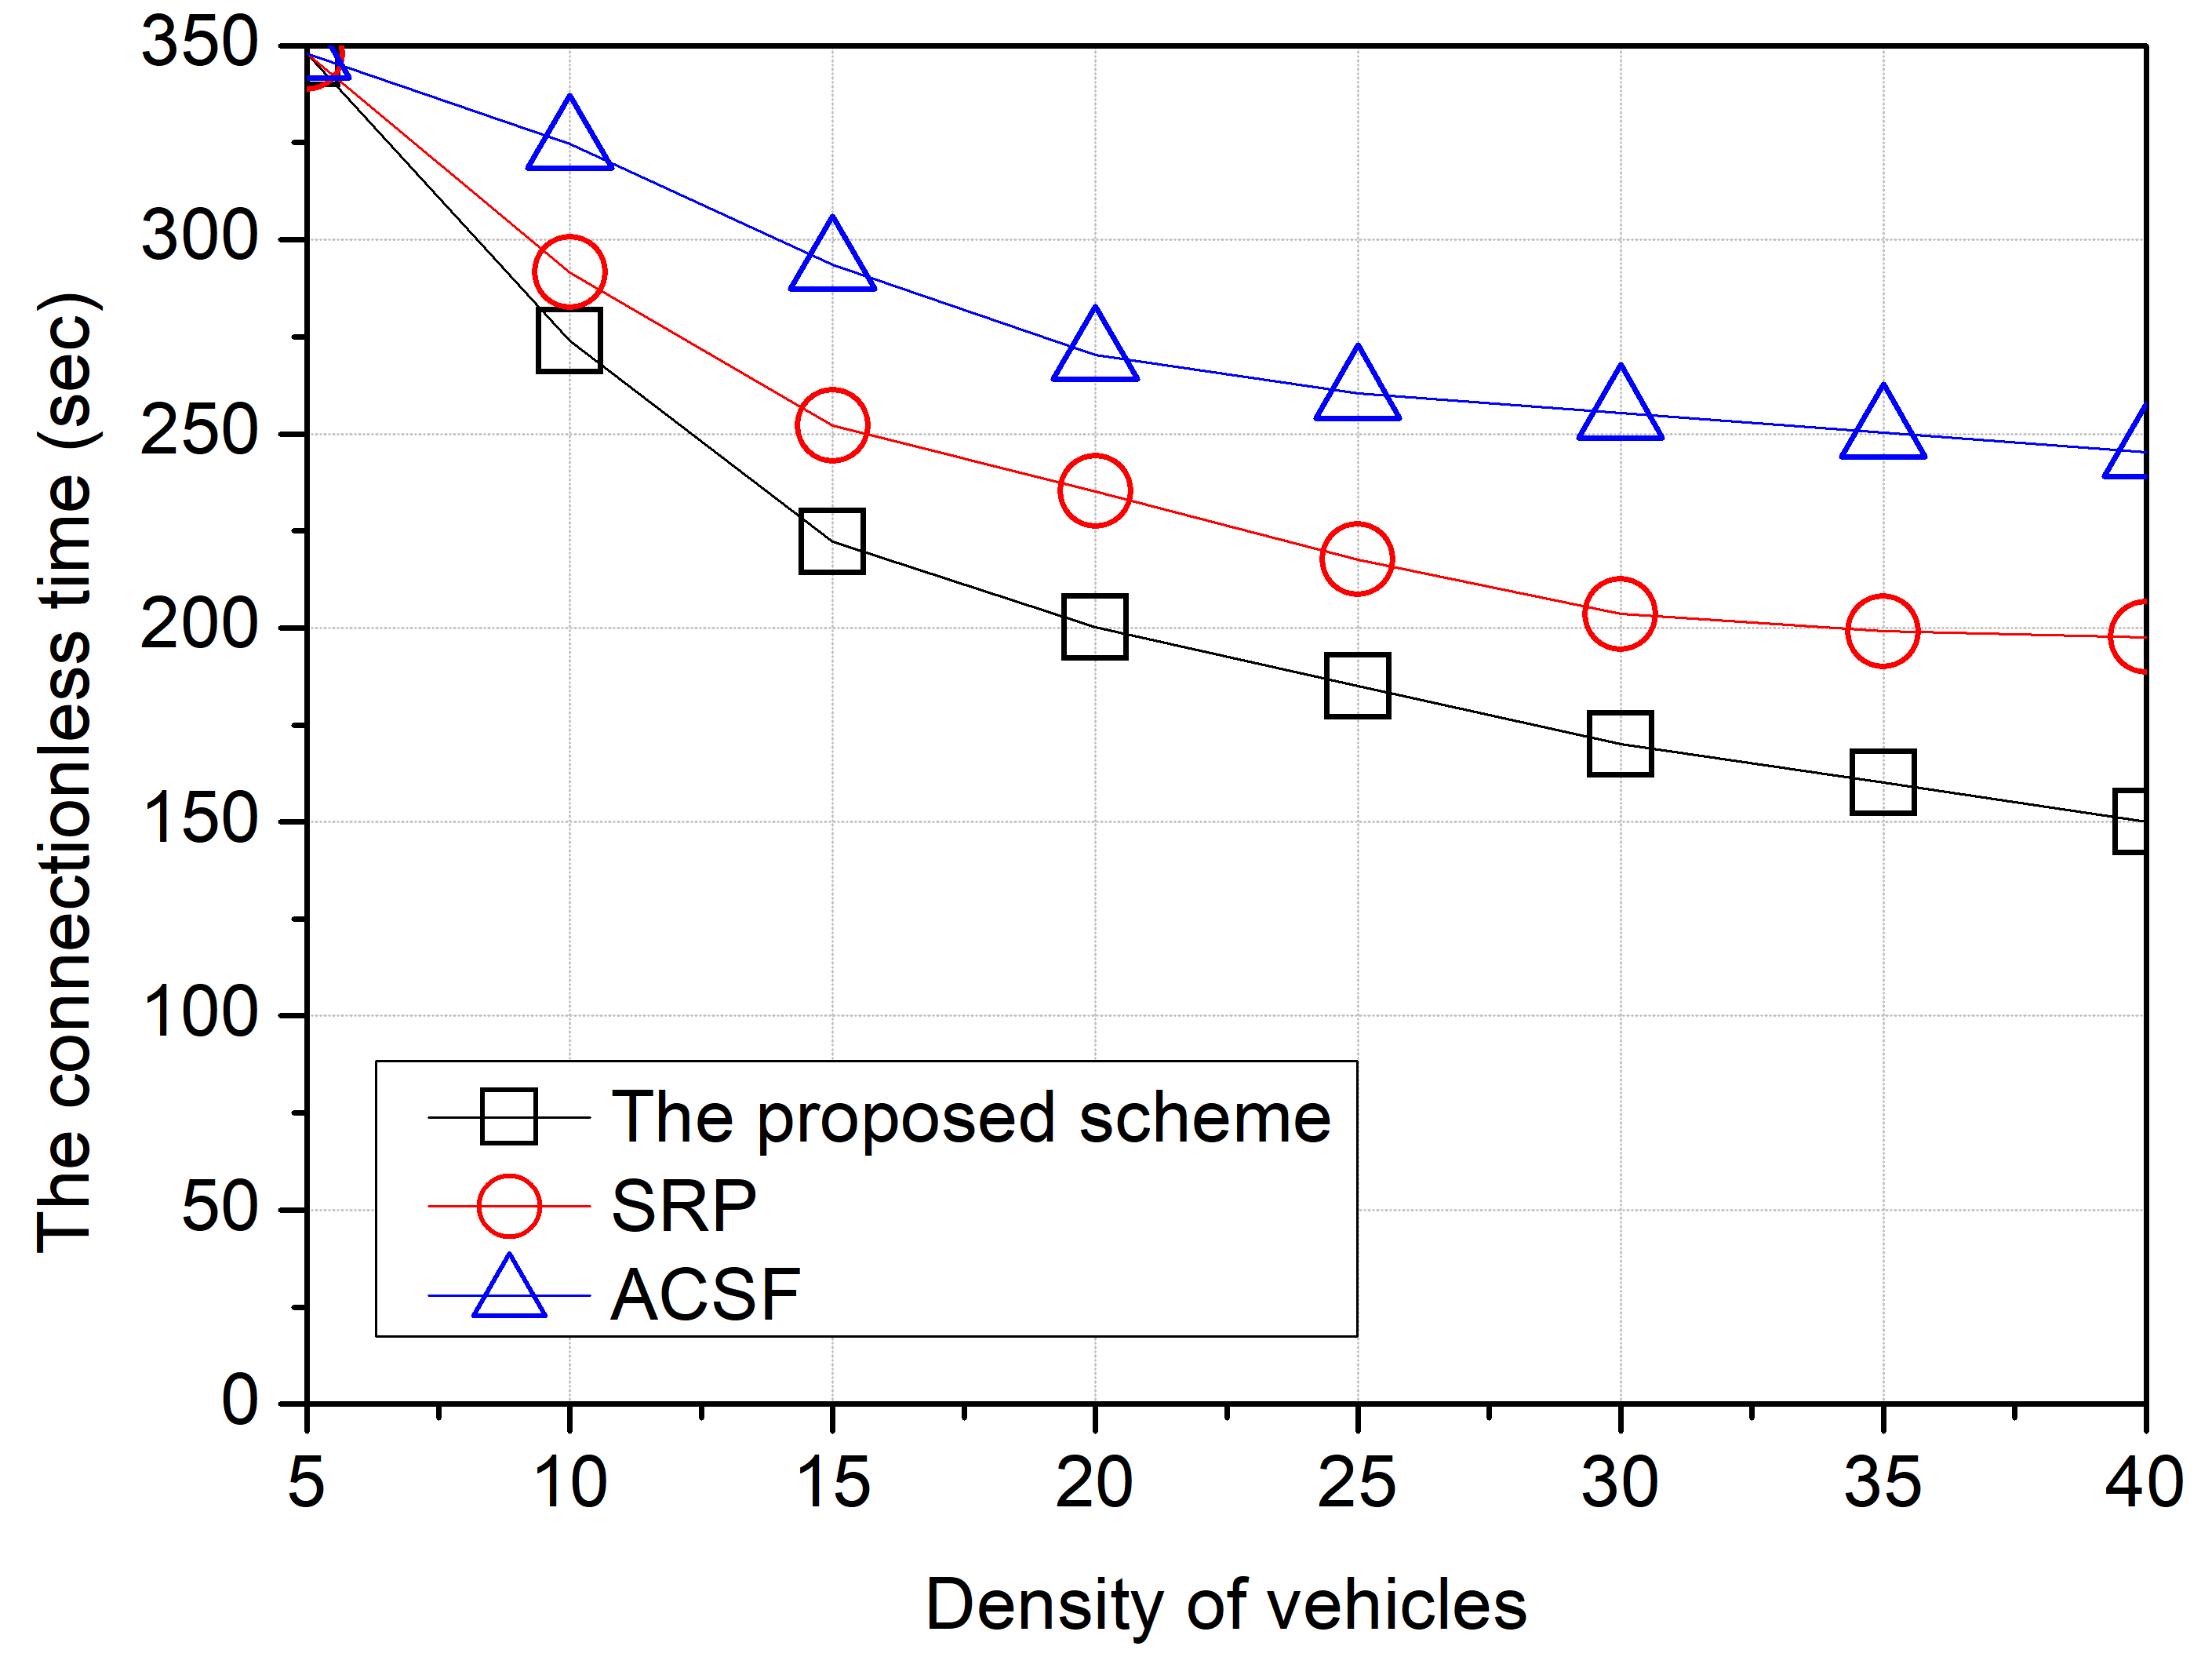
\includegraphics[width=.48\linewidth]{./graphs/DC.png}}
    \hspace{6pt}
    \raggedright \subfloat[\centering \label{fig8:b}]{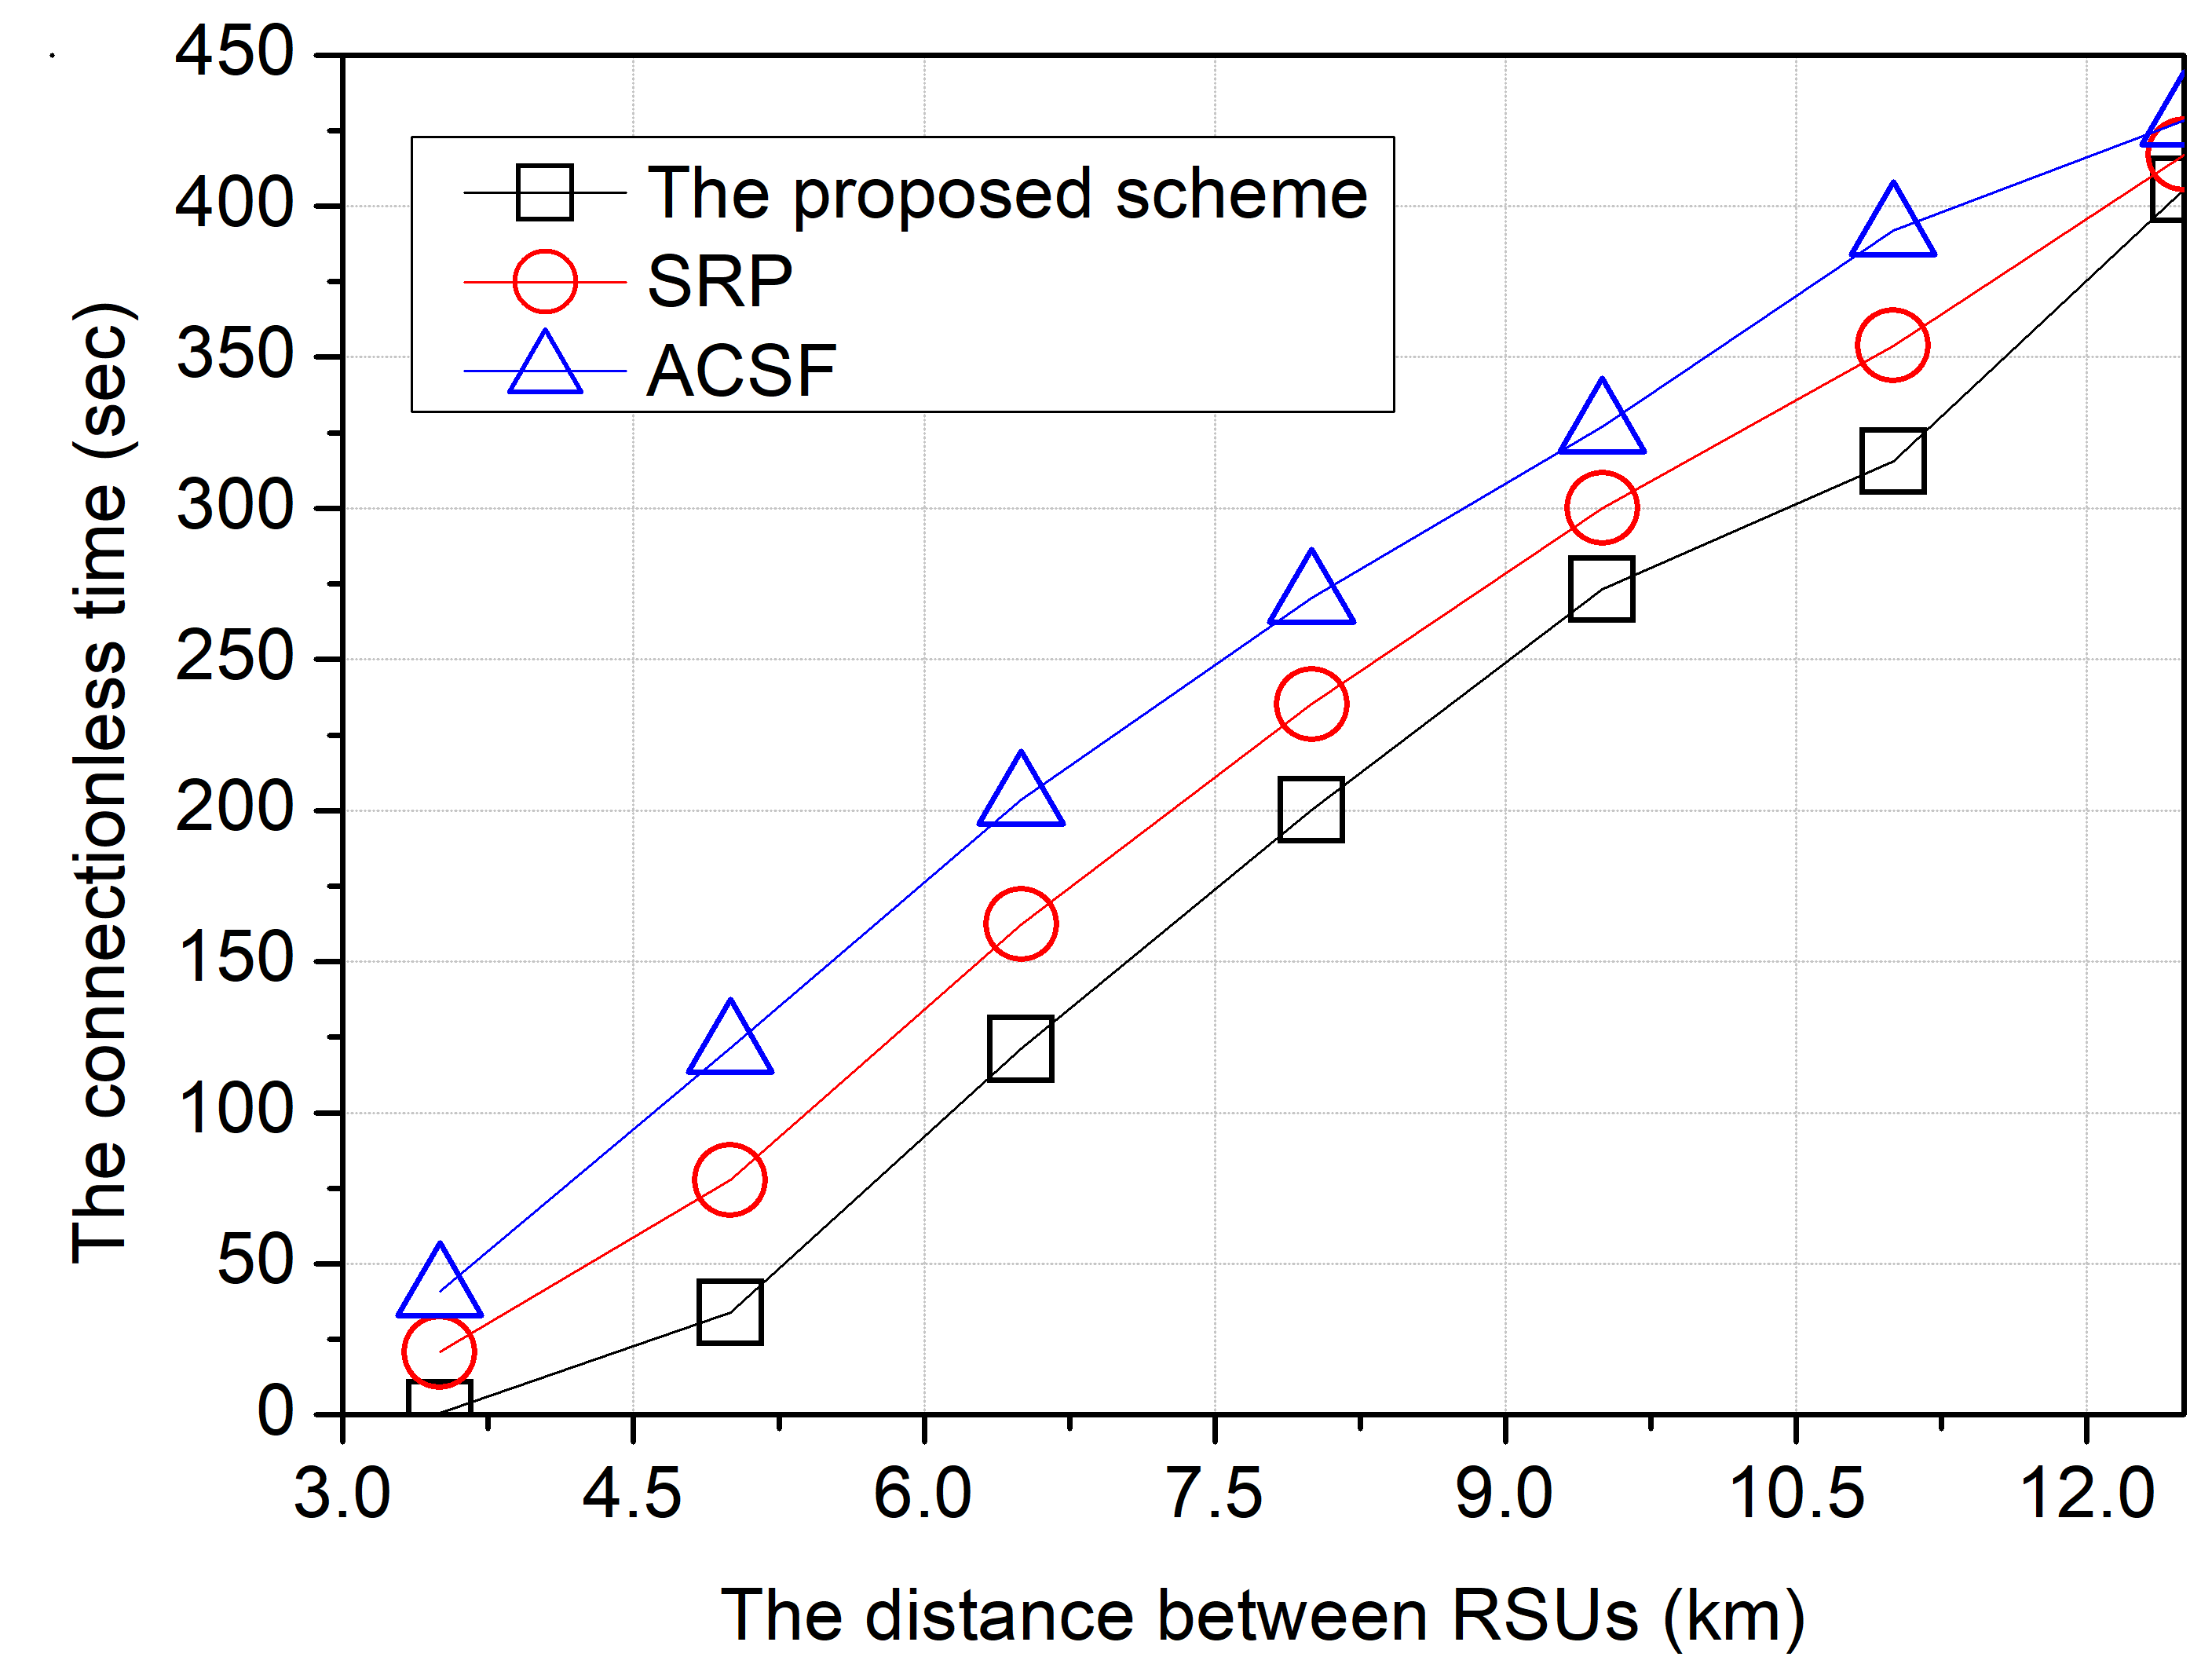
\includegraphics[width=.48\linewidth]{./graphs/LC.png}}
    \caption{The connectionless time according to (\textbf{a}) the density of vehicles; (\textbf{b}) the distance between~RSUs.}
    \label{fig:my_label2}
\end{figure}

Figure~\ref{fig:my_label2}b shows the connectionless time in relation to vehicle density. As~vehicle density increases, connectionless time decreases due to the greater availability of precaching vehicles. ACSF exhibits the highest connectionless time across all densities. Since it relies on a single precaching vehicle within a single-hop communication range, it often lacks sufficient candidate vehicles for data delivery, resulting in longer connectionless times. In~contrast, SRP demonstrates a lower connectionless time than ACSF by utilizing multiple precaching vehicles, which increases the number of candidates and reduces connectionless time. However, it still operates within a single-hop communication range, resulting in higher connectionless time compared to the proposed scheme. The~proposed scheme consistently achieves the lowest connectionless time across all densities. By~employing multiple precaching vehicles within a multi-hop communication range, it maximizes the number of candidate vehicles and minimizes connectionless time, thus providing the most efficient~performance.


Figure~\ref{fig:my_label3}a shows the dark area time in relation to the data rate. While increasing the data rate enables more data to be transmitted during connection time, it does not significantly impact dark area time due to the finite amount of data and the limited number of precaching vehicles. ACSF exhibits a high dark area time of approximately 250 s across various data rates, as~it relies on a single precaching vehicle, resulting in the highest dark area time. In~comparison, SRP maintains a constant dark area time of about 50~s, which is lower than that of ACSF. By~utilizing multiple precaching vehicles, SRP reduces the dark area time relative to ACSF, although~it remains constrained by the single-hop communication range. The~proposed scheme achieves the lowest dark area time by employing multiple precaching vehicles within a multi-hop communication range. This efficient precaching strategy effectively minimizes dark area time, regardless of the data~rate.





Figure~\ref{fig:my_label3}b shows the dark area time in relation to the size of the requested content. As~the content size increases, more precaching vehicles are required, leading to larger dark areas and increased dark area time. ACSF relies on a single precaching vehicle, resulting in a constant dark area time regardless of content size due to its limited precaching capacity. In~contrast, SRP employs multiple relaying vehicles within a single-hop communication range. However, the~insufficient number of candidate vehicles causes the dark area time to rise sharply as content sizes increase. The~proposed scheme utilizes multiple precaching vehicles within a multi-hop communication range, enabling continuous content delivery even in dark areas. Consequently, dark area time remains constant, irrespective of content~size.

\vspace{-8pt}
\begin{figure}[H]
    \centering \subfloat[\centering \label{fig9:a}]{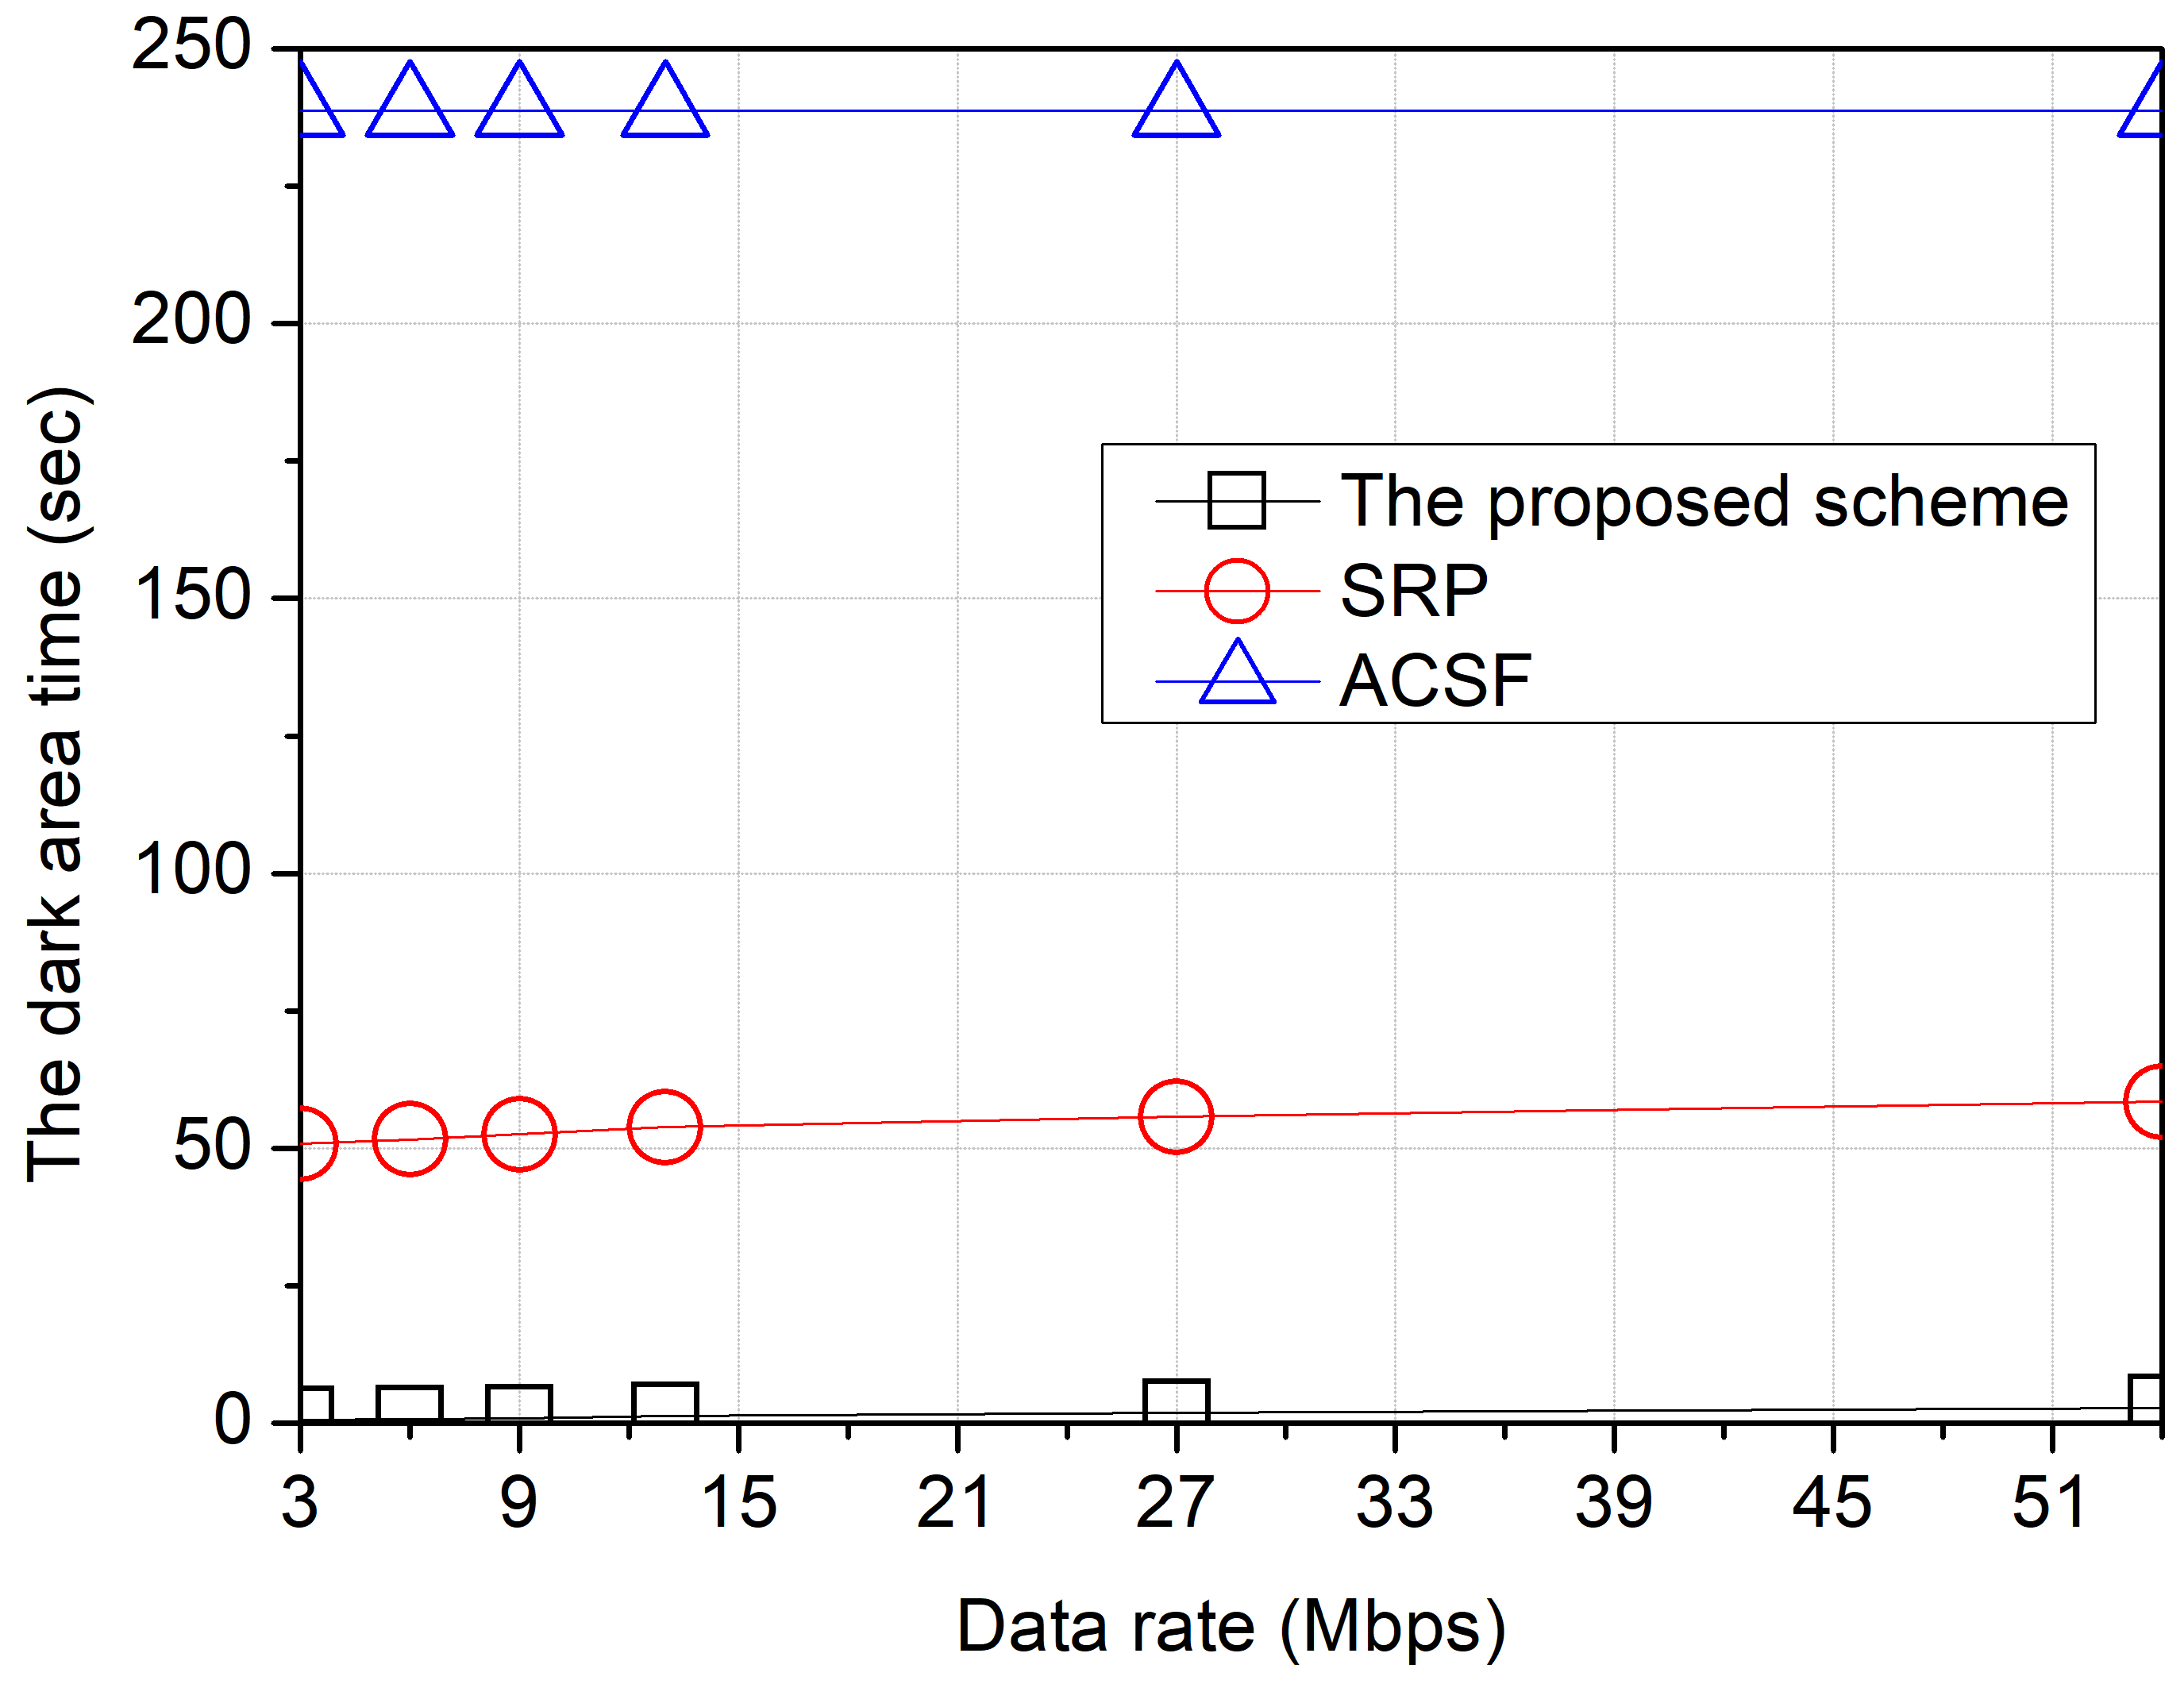
\includegraphics[width=.46\linewidth]{./graphs/RD.png}}
  \vspace{-6pt}  \centering \subfloat[\centering \label{fig9:b}]{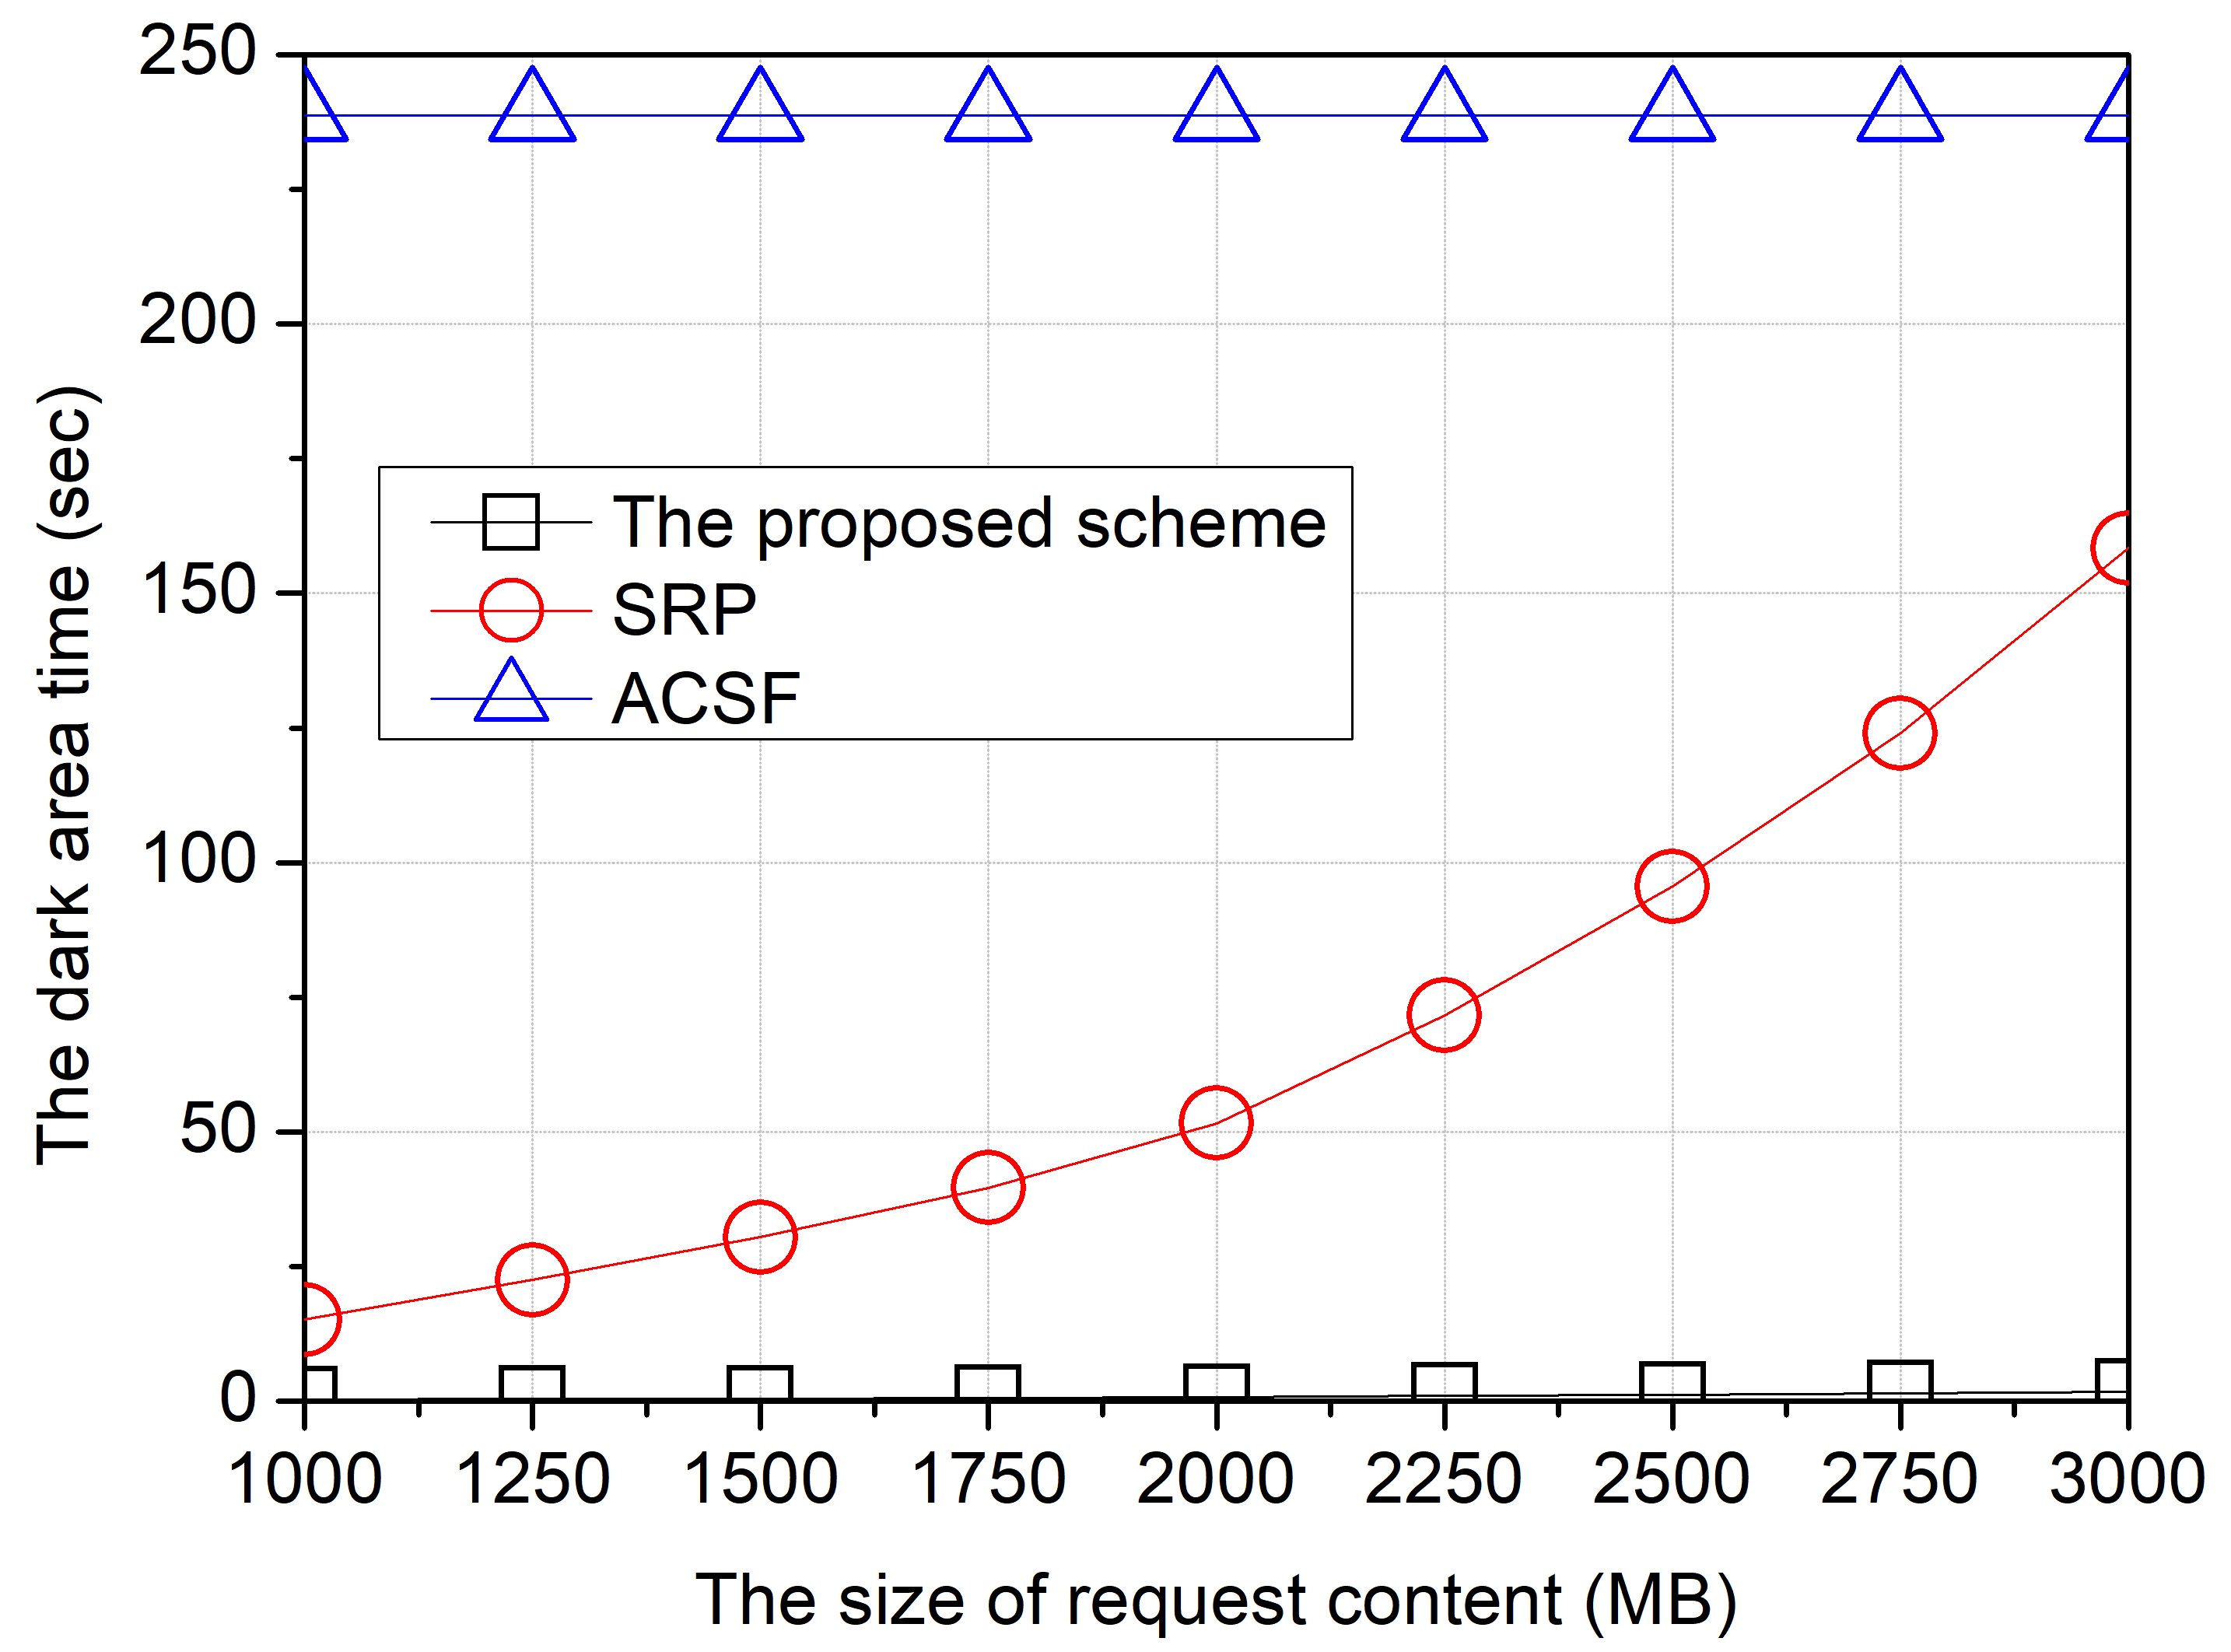
\includegraphics[width=.48\linewidth]{./graphs/SD.png}}
    \\
    \centering \subfloat[\centering \label{fig9:c}]{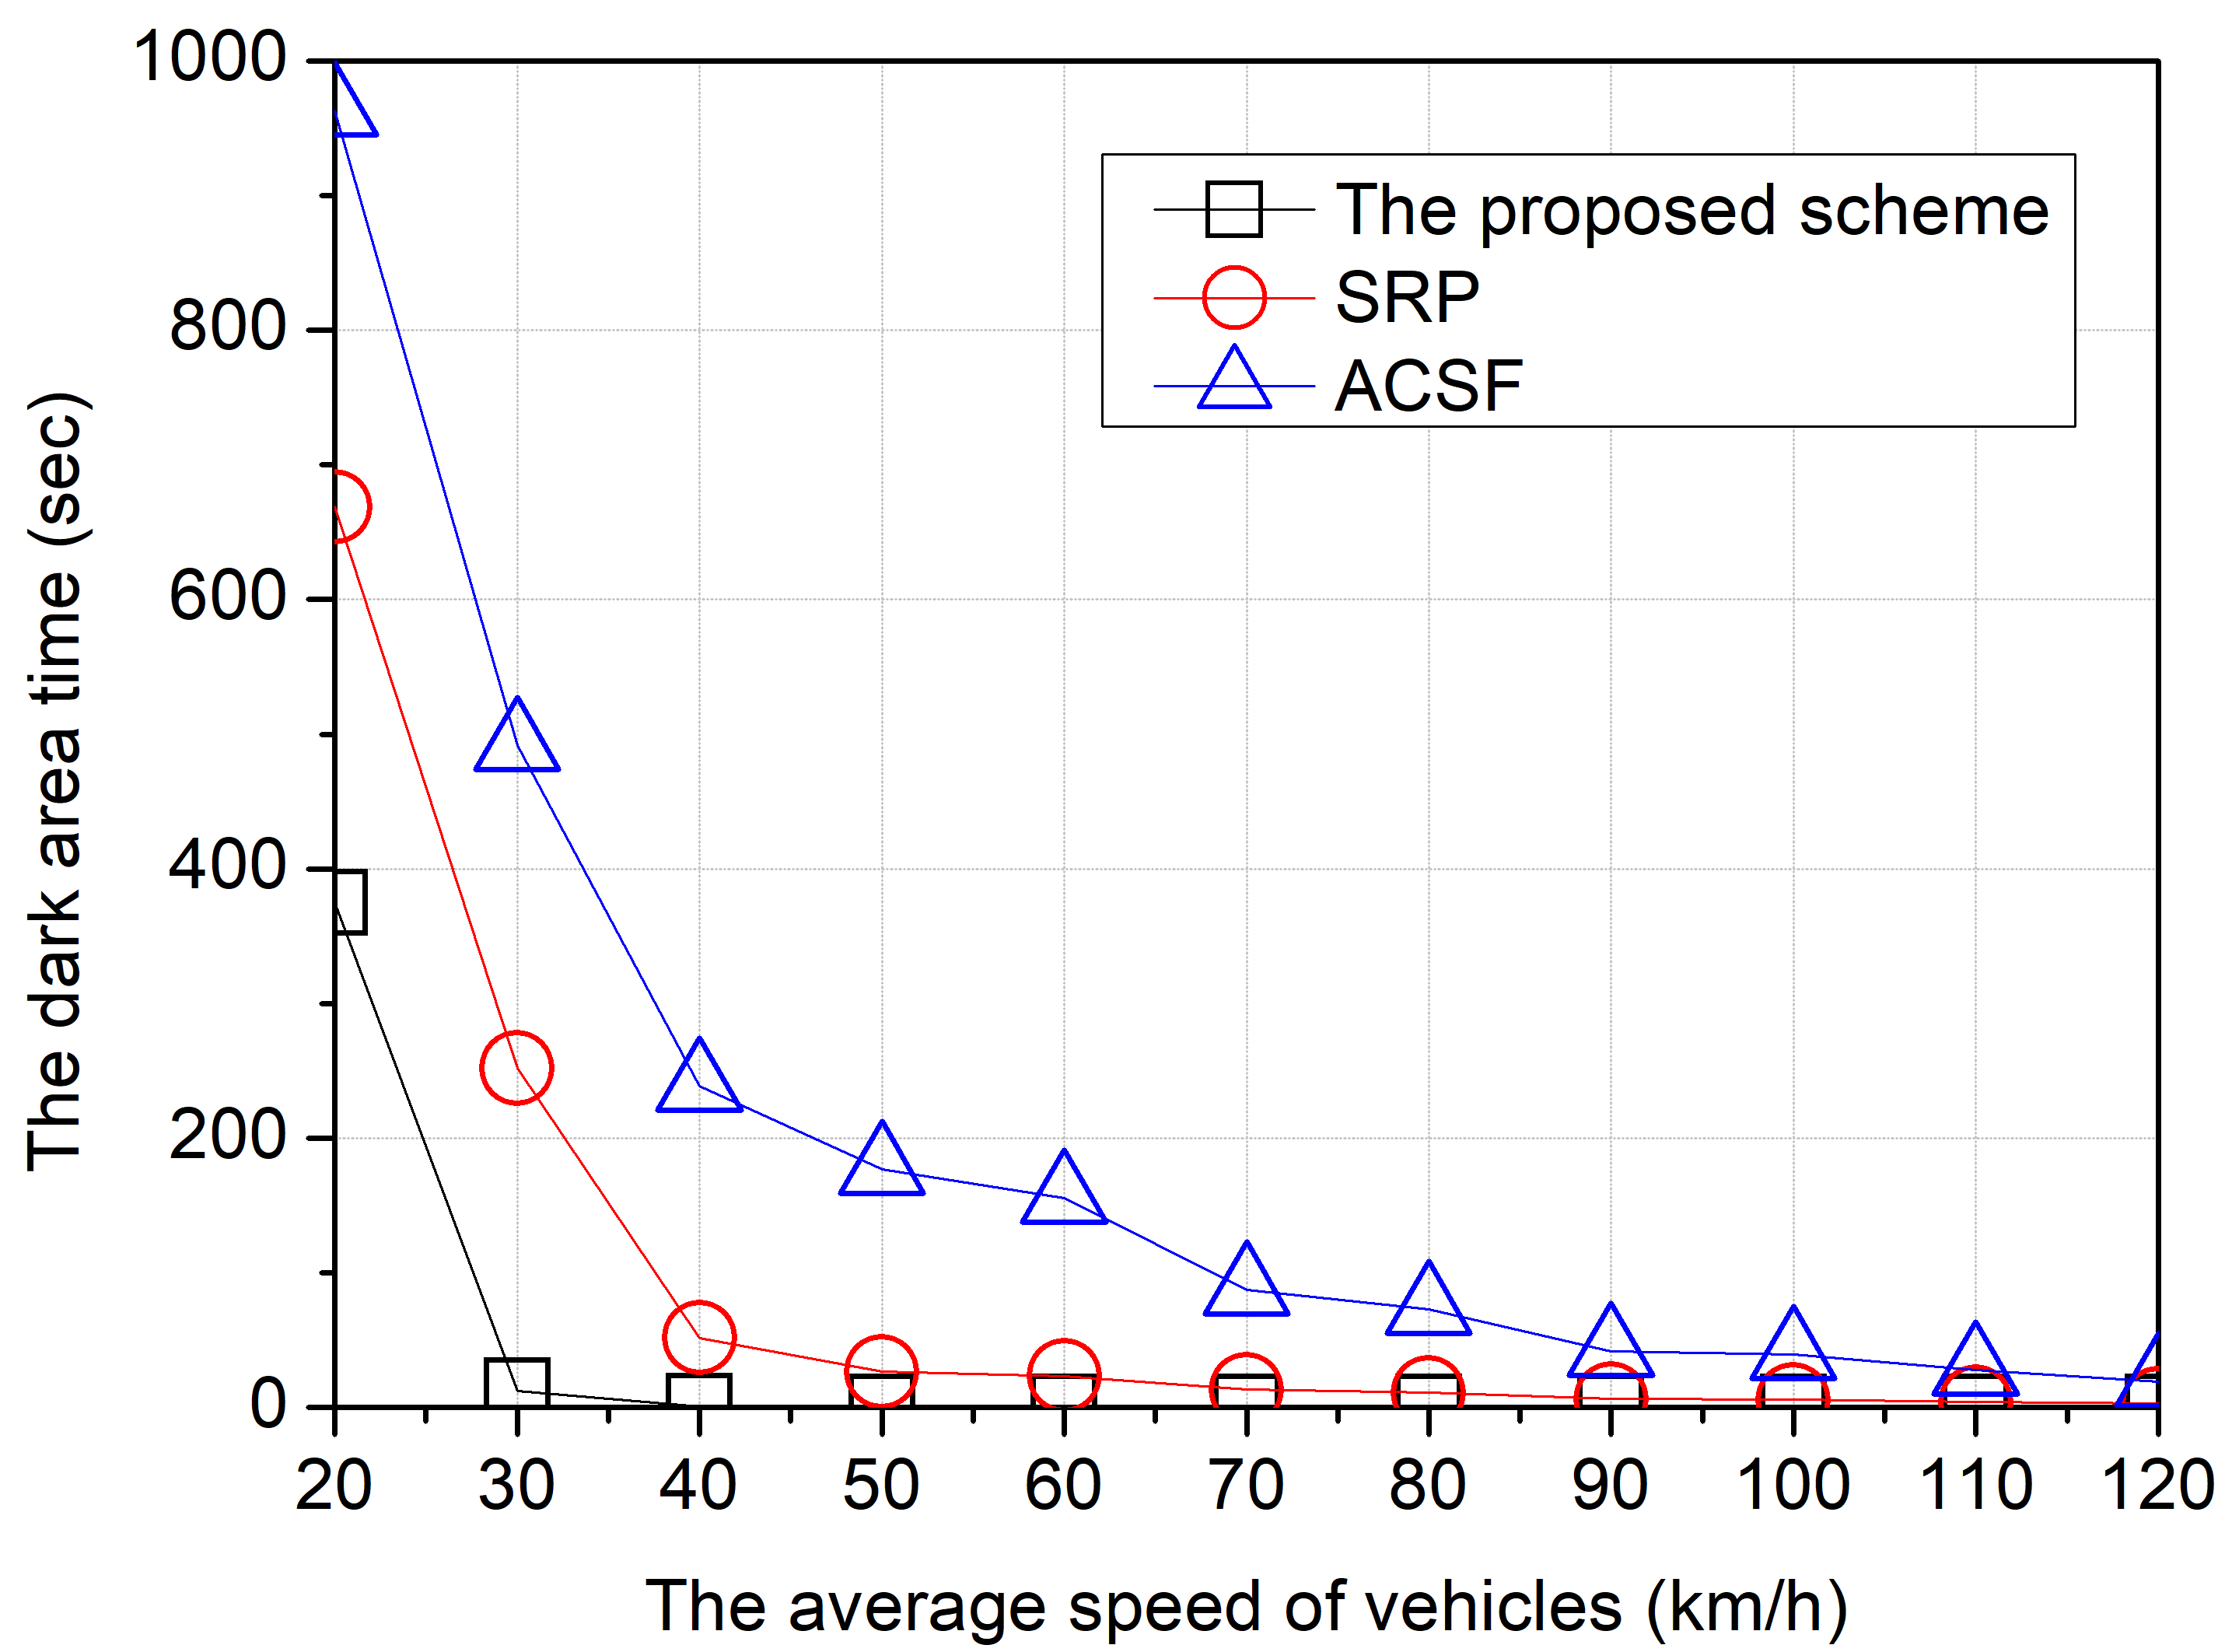
\includegraphics[width=.48\linewidth]{./graphs/VD.png}}
    \caption{The dark area time according to (\textbf{a}) the data rate; (\textbf{b}) the size of the requested content; (\textbf{c}) the average speed of~vehicles.}
    \label{fig:my_label3}
\end{figure}

Figure~\ref{fig:my_label3}c shows the dark area time as a function of the average speed of vehicles. As~vehicle speed increases, connection times with RSUs and relay vehicles shorten, leading to a decrease in dark area time since vehicles pass through dark areas more quickly. ACSF exhibits a high dark area time at 20 km/h; although it decreases with higher speeds, it remains the highest compared to the other schemes. SRP also shows elevated dark area time at speeds of 40 km/h or less, but~it decreases sharply with increasing speed, approaching zero at speeds of 50 km/h or more. The~proposed scheme demonstrates a high dark area time below 30 km/h, but this falls to nearly zero at speeds above 30 km/h, indicating the most efficient performance at higher~speeds.


Figure~\ref{fig:my_label4}a shows the connectionless time as a function of data rate. Initially, as~the data rate increases, the~connectionless time rises due to insufficient content delivery time, but stabilizes beyond a data rate of 15. ACSF employs a single precaching vehicle within a single-hop communication range, leading to a decrease in connectionless time at higher data rates, although~it remains elevated at lower data rates compared to the other schemes. SRP utilizes multiple precaching vehicles, resulting in lower connectionless time than ACSF. Although~connectionless time decreases with higher data rates, it remains higher than that of the proposed scheme due to its single-hop communication limitations. The~proposed scheme experiences a noticeable increase in connectionless time at low data rates; however, beyond~a data rate of 15, it effectively uses multiple precaching vehicles in a multi-hop communication range, achieving the lowest connectionless time among all~schemes.








Figure~\ref{fig:my_label4}b shows the connectionless time as a function of the size of the requested content. As~the size of the requested content increases, more precaching vehicles are required, leading to potential dark areas and an increase in connectionless time. ACSF exhibits a constant connectionless time regardless of the size of the requested content because it relies solely on a single precaching vehicle. In~contrast, SRP employs multiple precaching vehicles within a single-hop range. As~the size of the requested content increases, the~limited number of available precaching vehicles results in a significant rise in connectionless time. Although~connectionless time does increase with content size, the~proposed scheme maintains a relatively lower connectionless time compared to both SRP and ACSF. This scheme effectively delivers larger amounts of content through multiple precaching vehicles in a multi-hop communication~range.








Figure~\ref{fig:my_label4}c shows the connectionless time as a function of the average speed of vehicles. Faster vehicle speeds shorten connection times with RSUs and precaching vehicles, thereby reducing the connectionless time as vehicles quickly pass through dark areas. ACSF exhibits higher connectionless time than the other schemes; however, it decreases as vehicle speed increases due to its reliance on a single precaching vehicle. In~contrast, SRP employs multiple precaching vehicles, resulting in lower connectionless time compared to ACSF. Nevertheless, its connectionless time remains higher than that of the proposed scheme due to its single-hop communication approach. The~proposed scheme utilizes multiple precaching vehicles in a multi-hop communication range, ensuring stable content delivery and achieving the lowest connectionless time across varying vehicle~speeds.




\vspace{-8pt}
\begin{figure}[H]
    \centering \subfloat[\centering \label{fig10:a}]{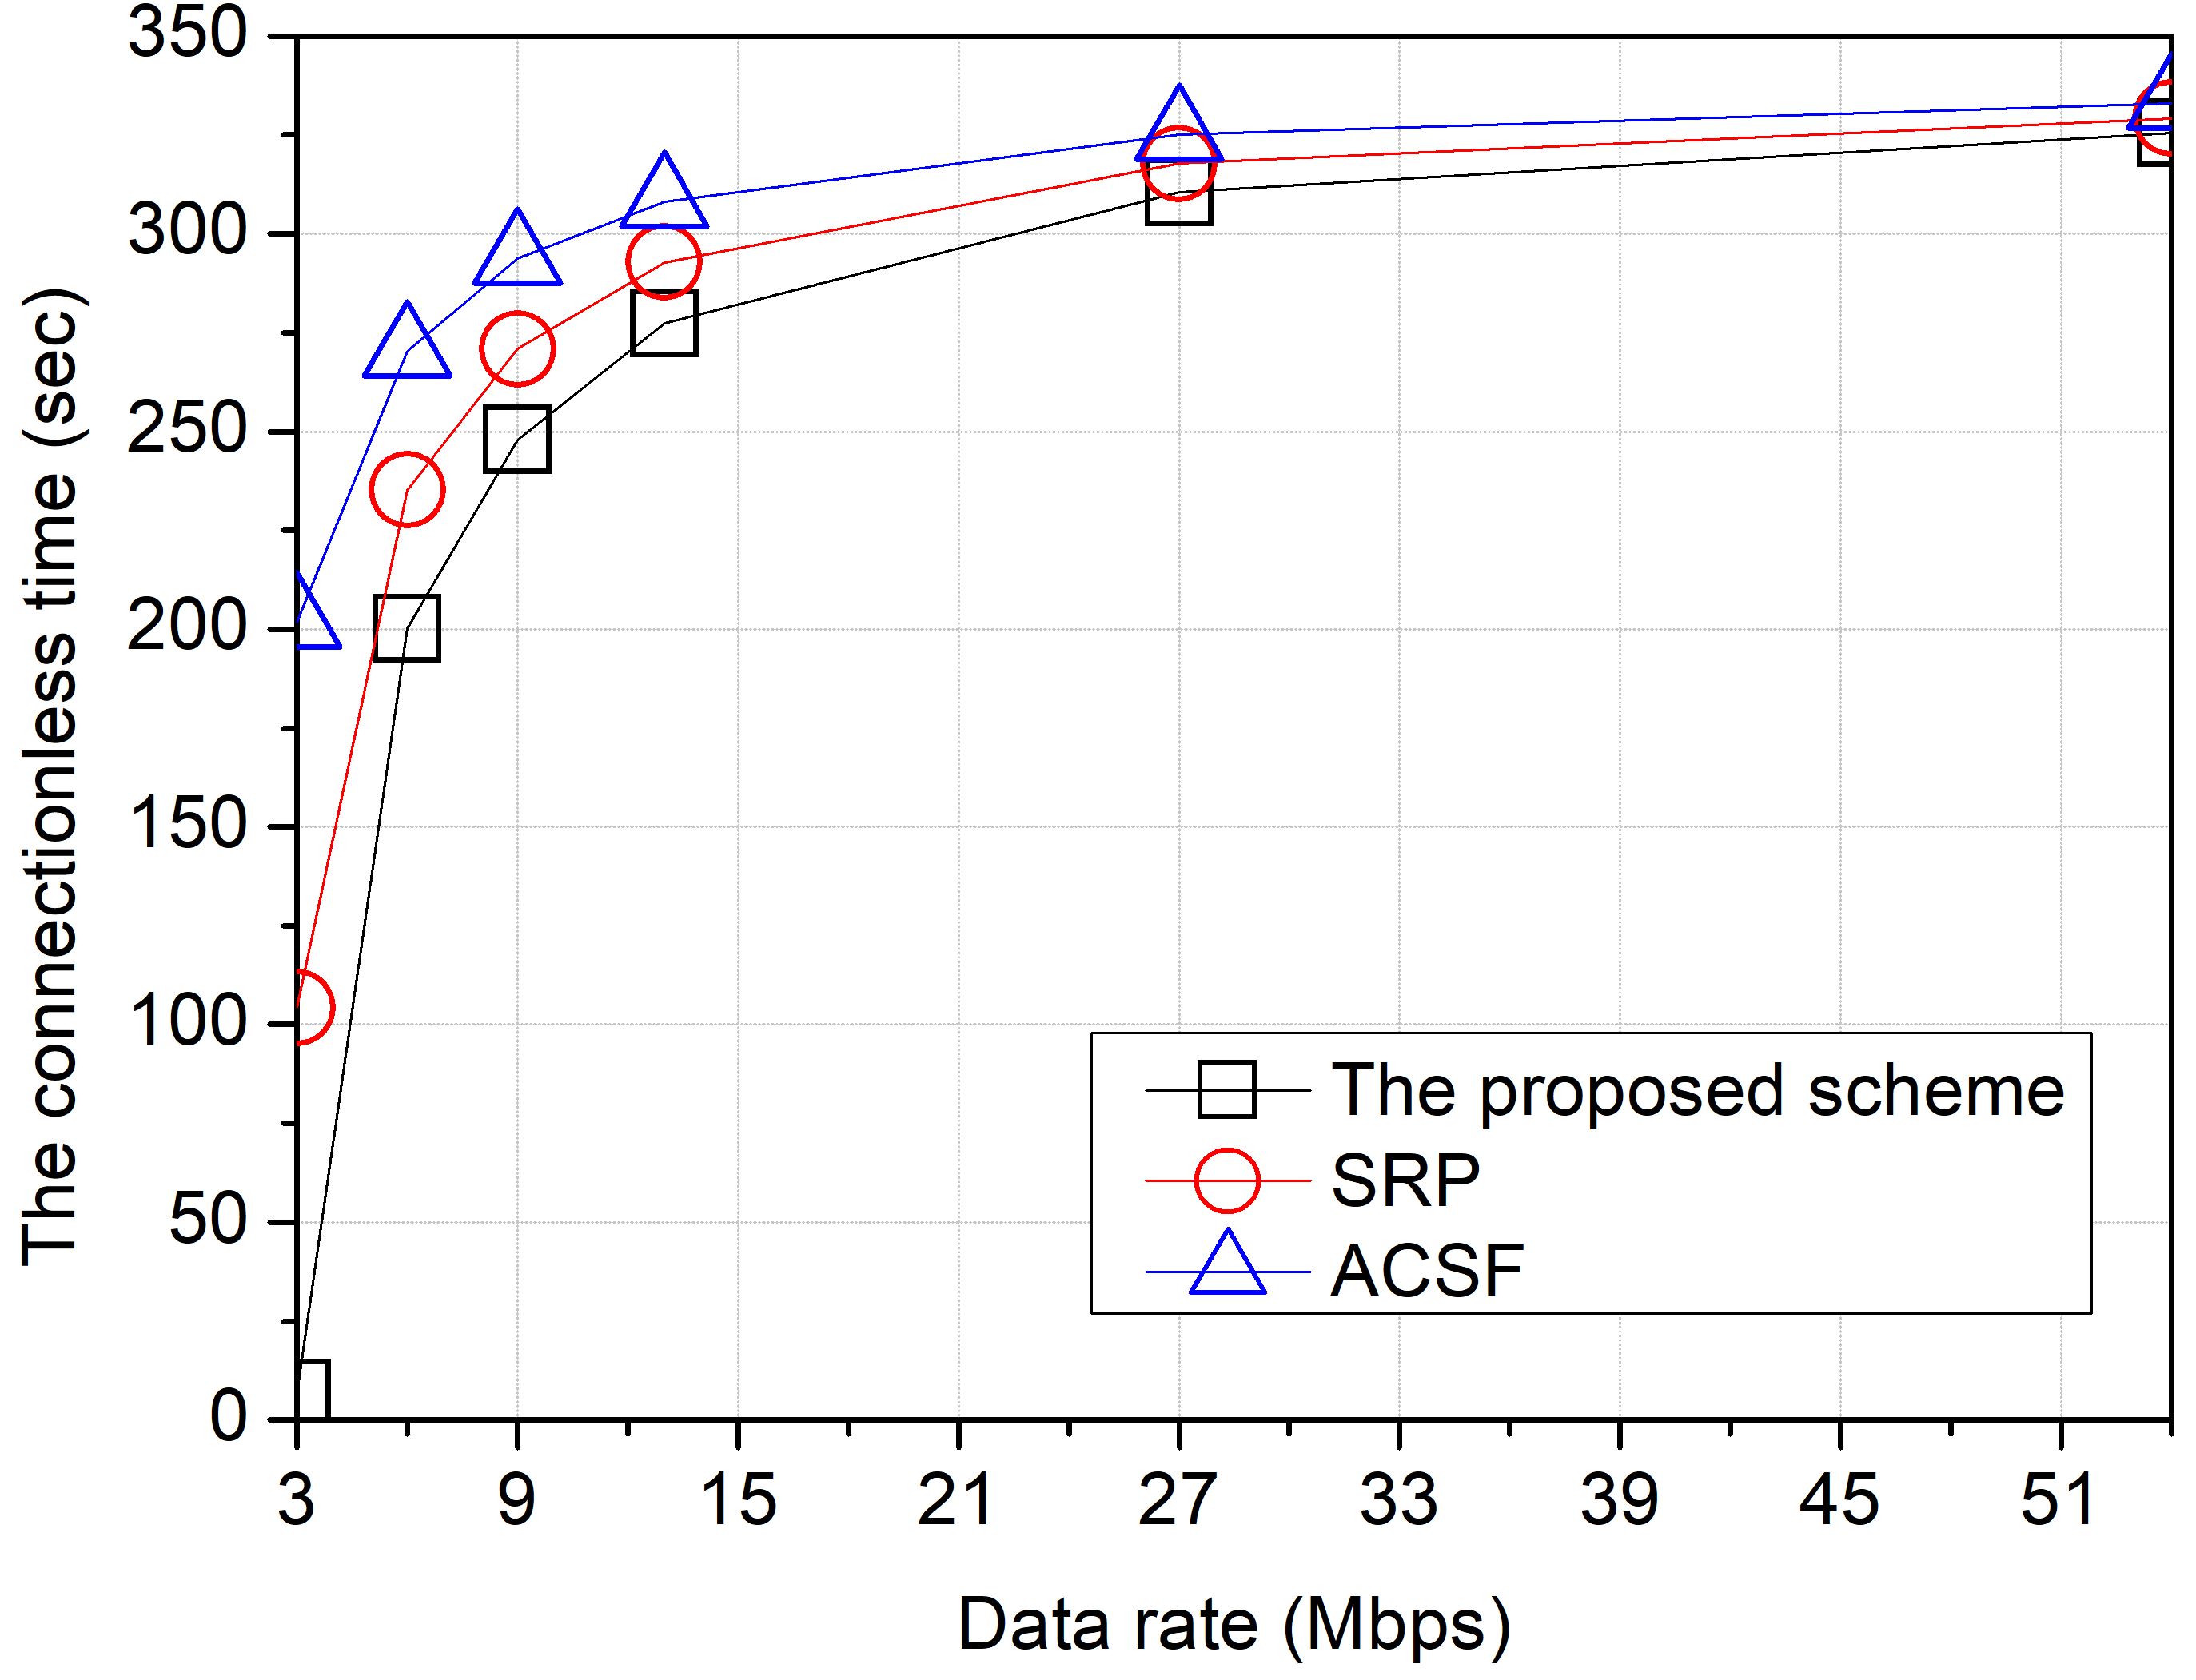
\includegraphics[width=.48\linewidth]{./graphs/RC.png}}
    \centering \subfloat[\centering \label{fig10:b}]{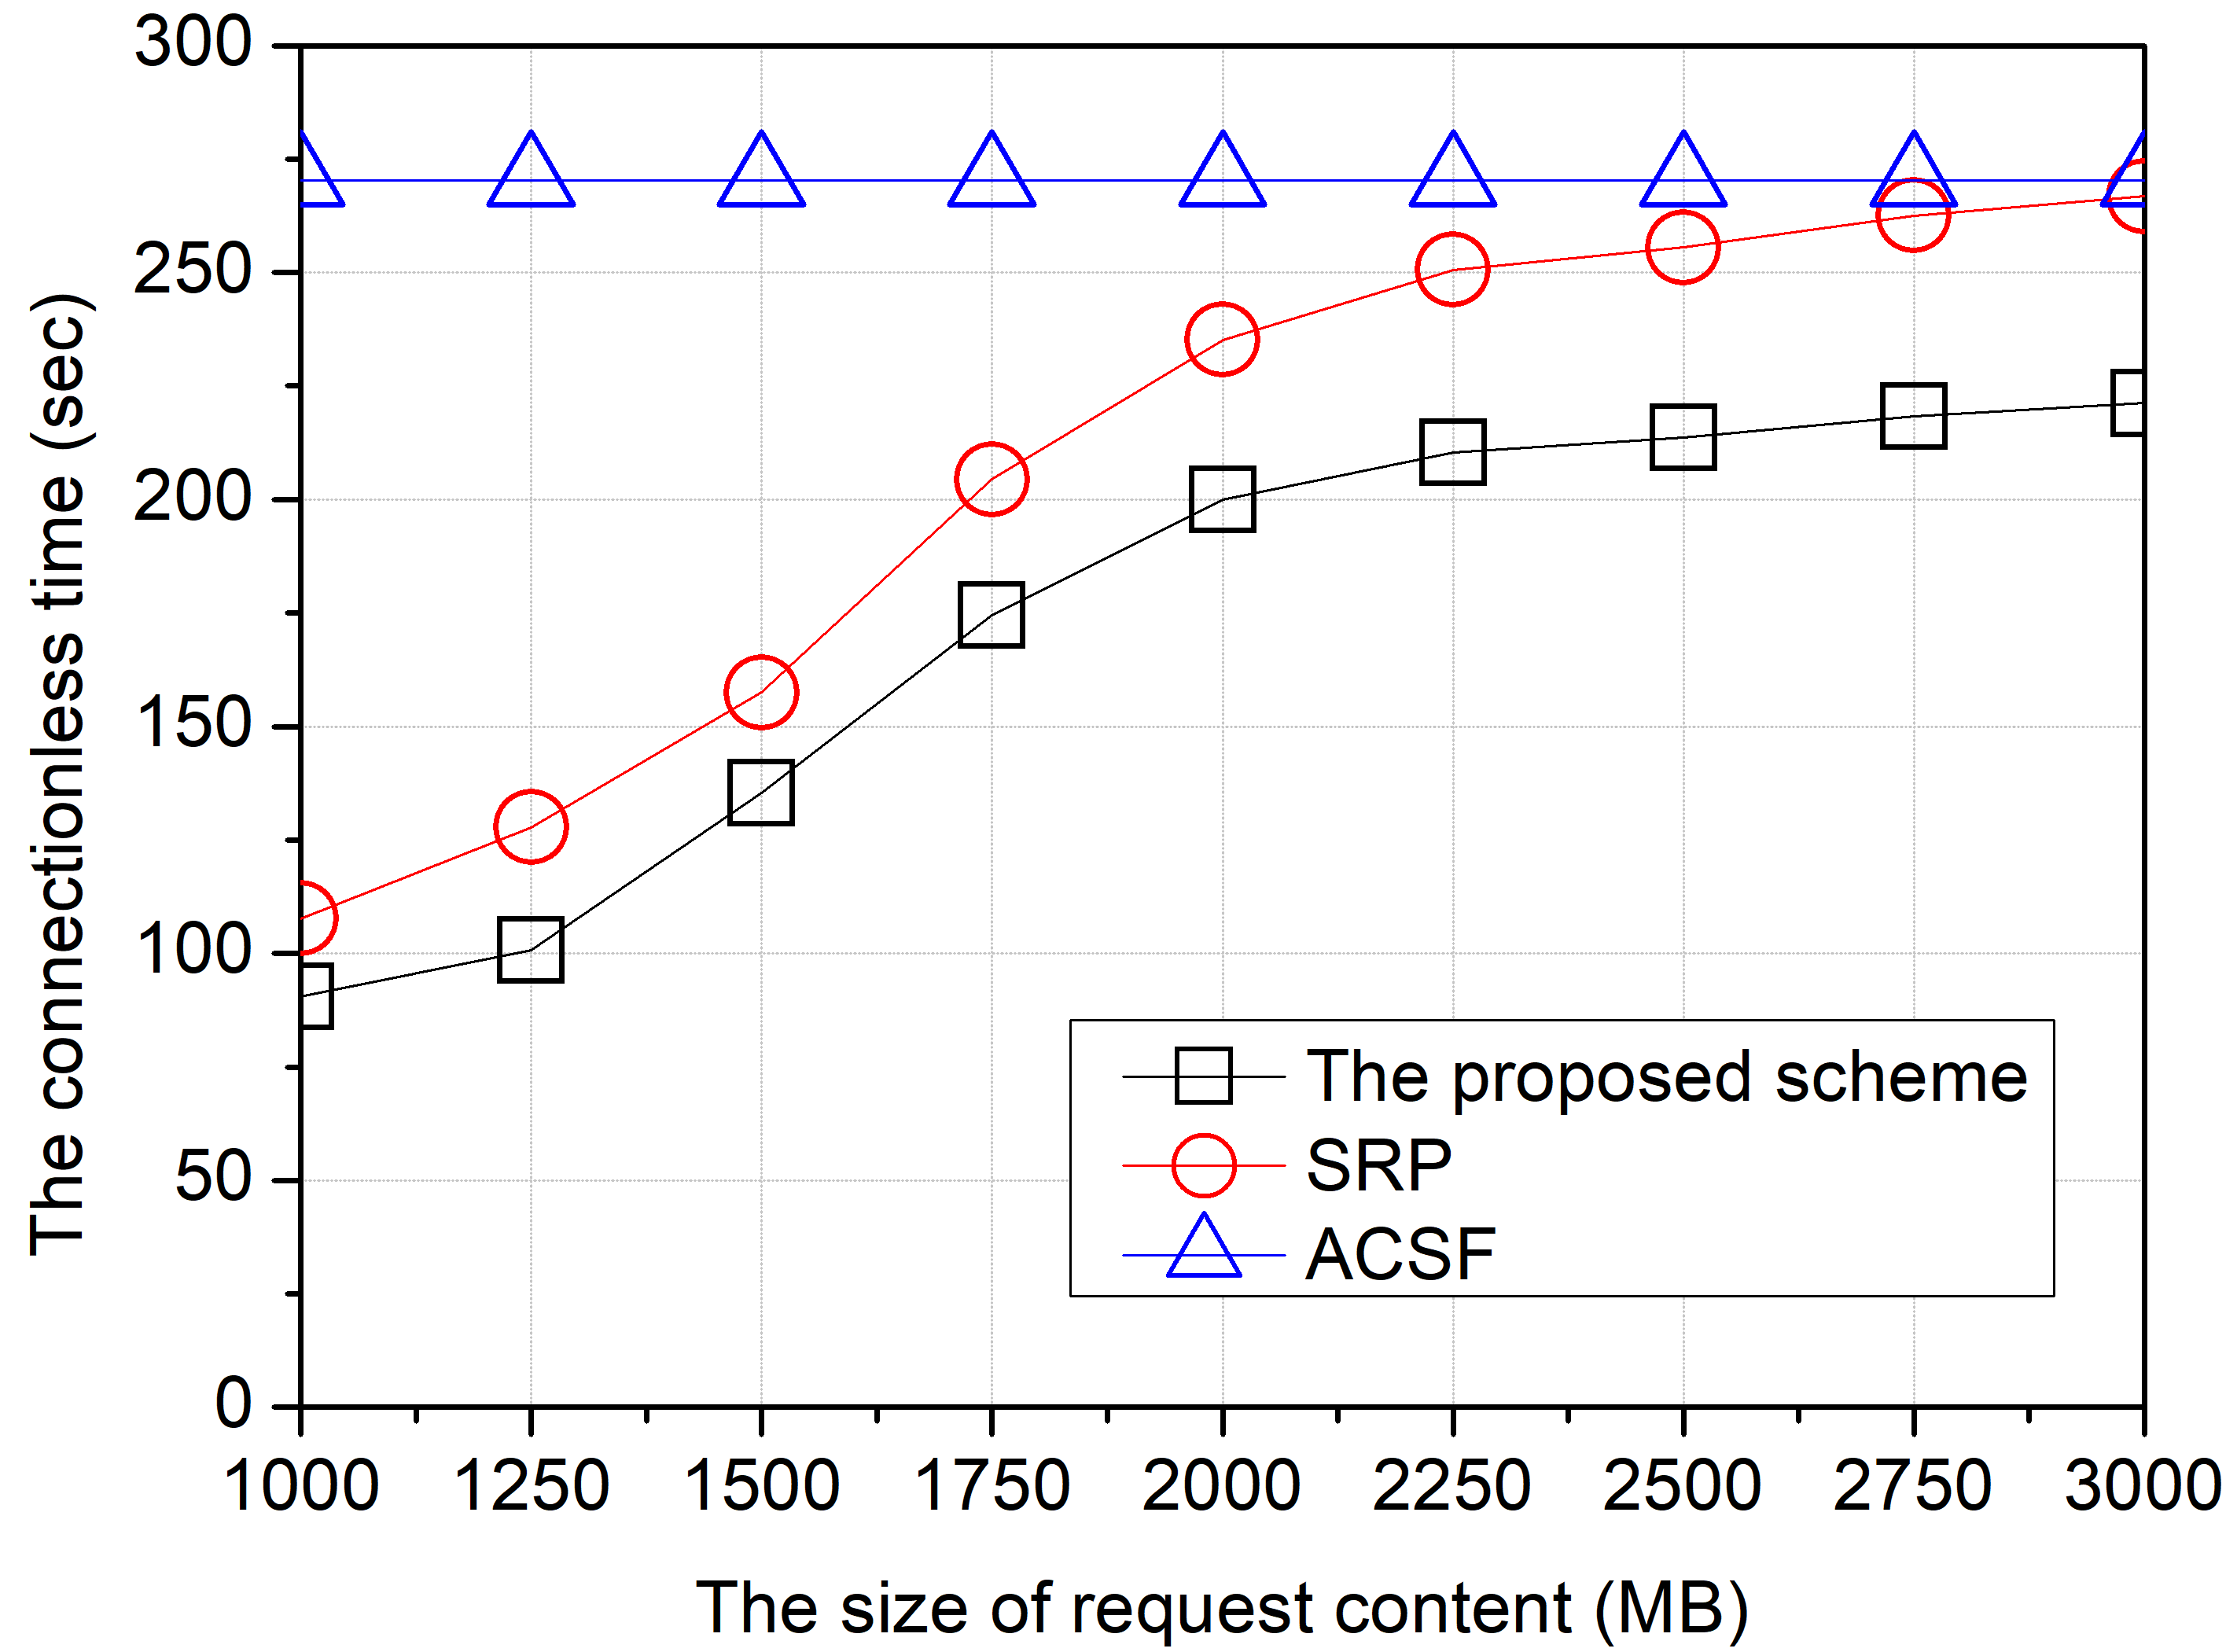
\includegraphics[width=.5\linewidth]{./graphs/SC.png}}
    \\
    \centering \subfloat[\centering \label{fig10:c}]{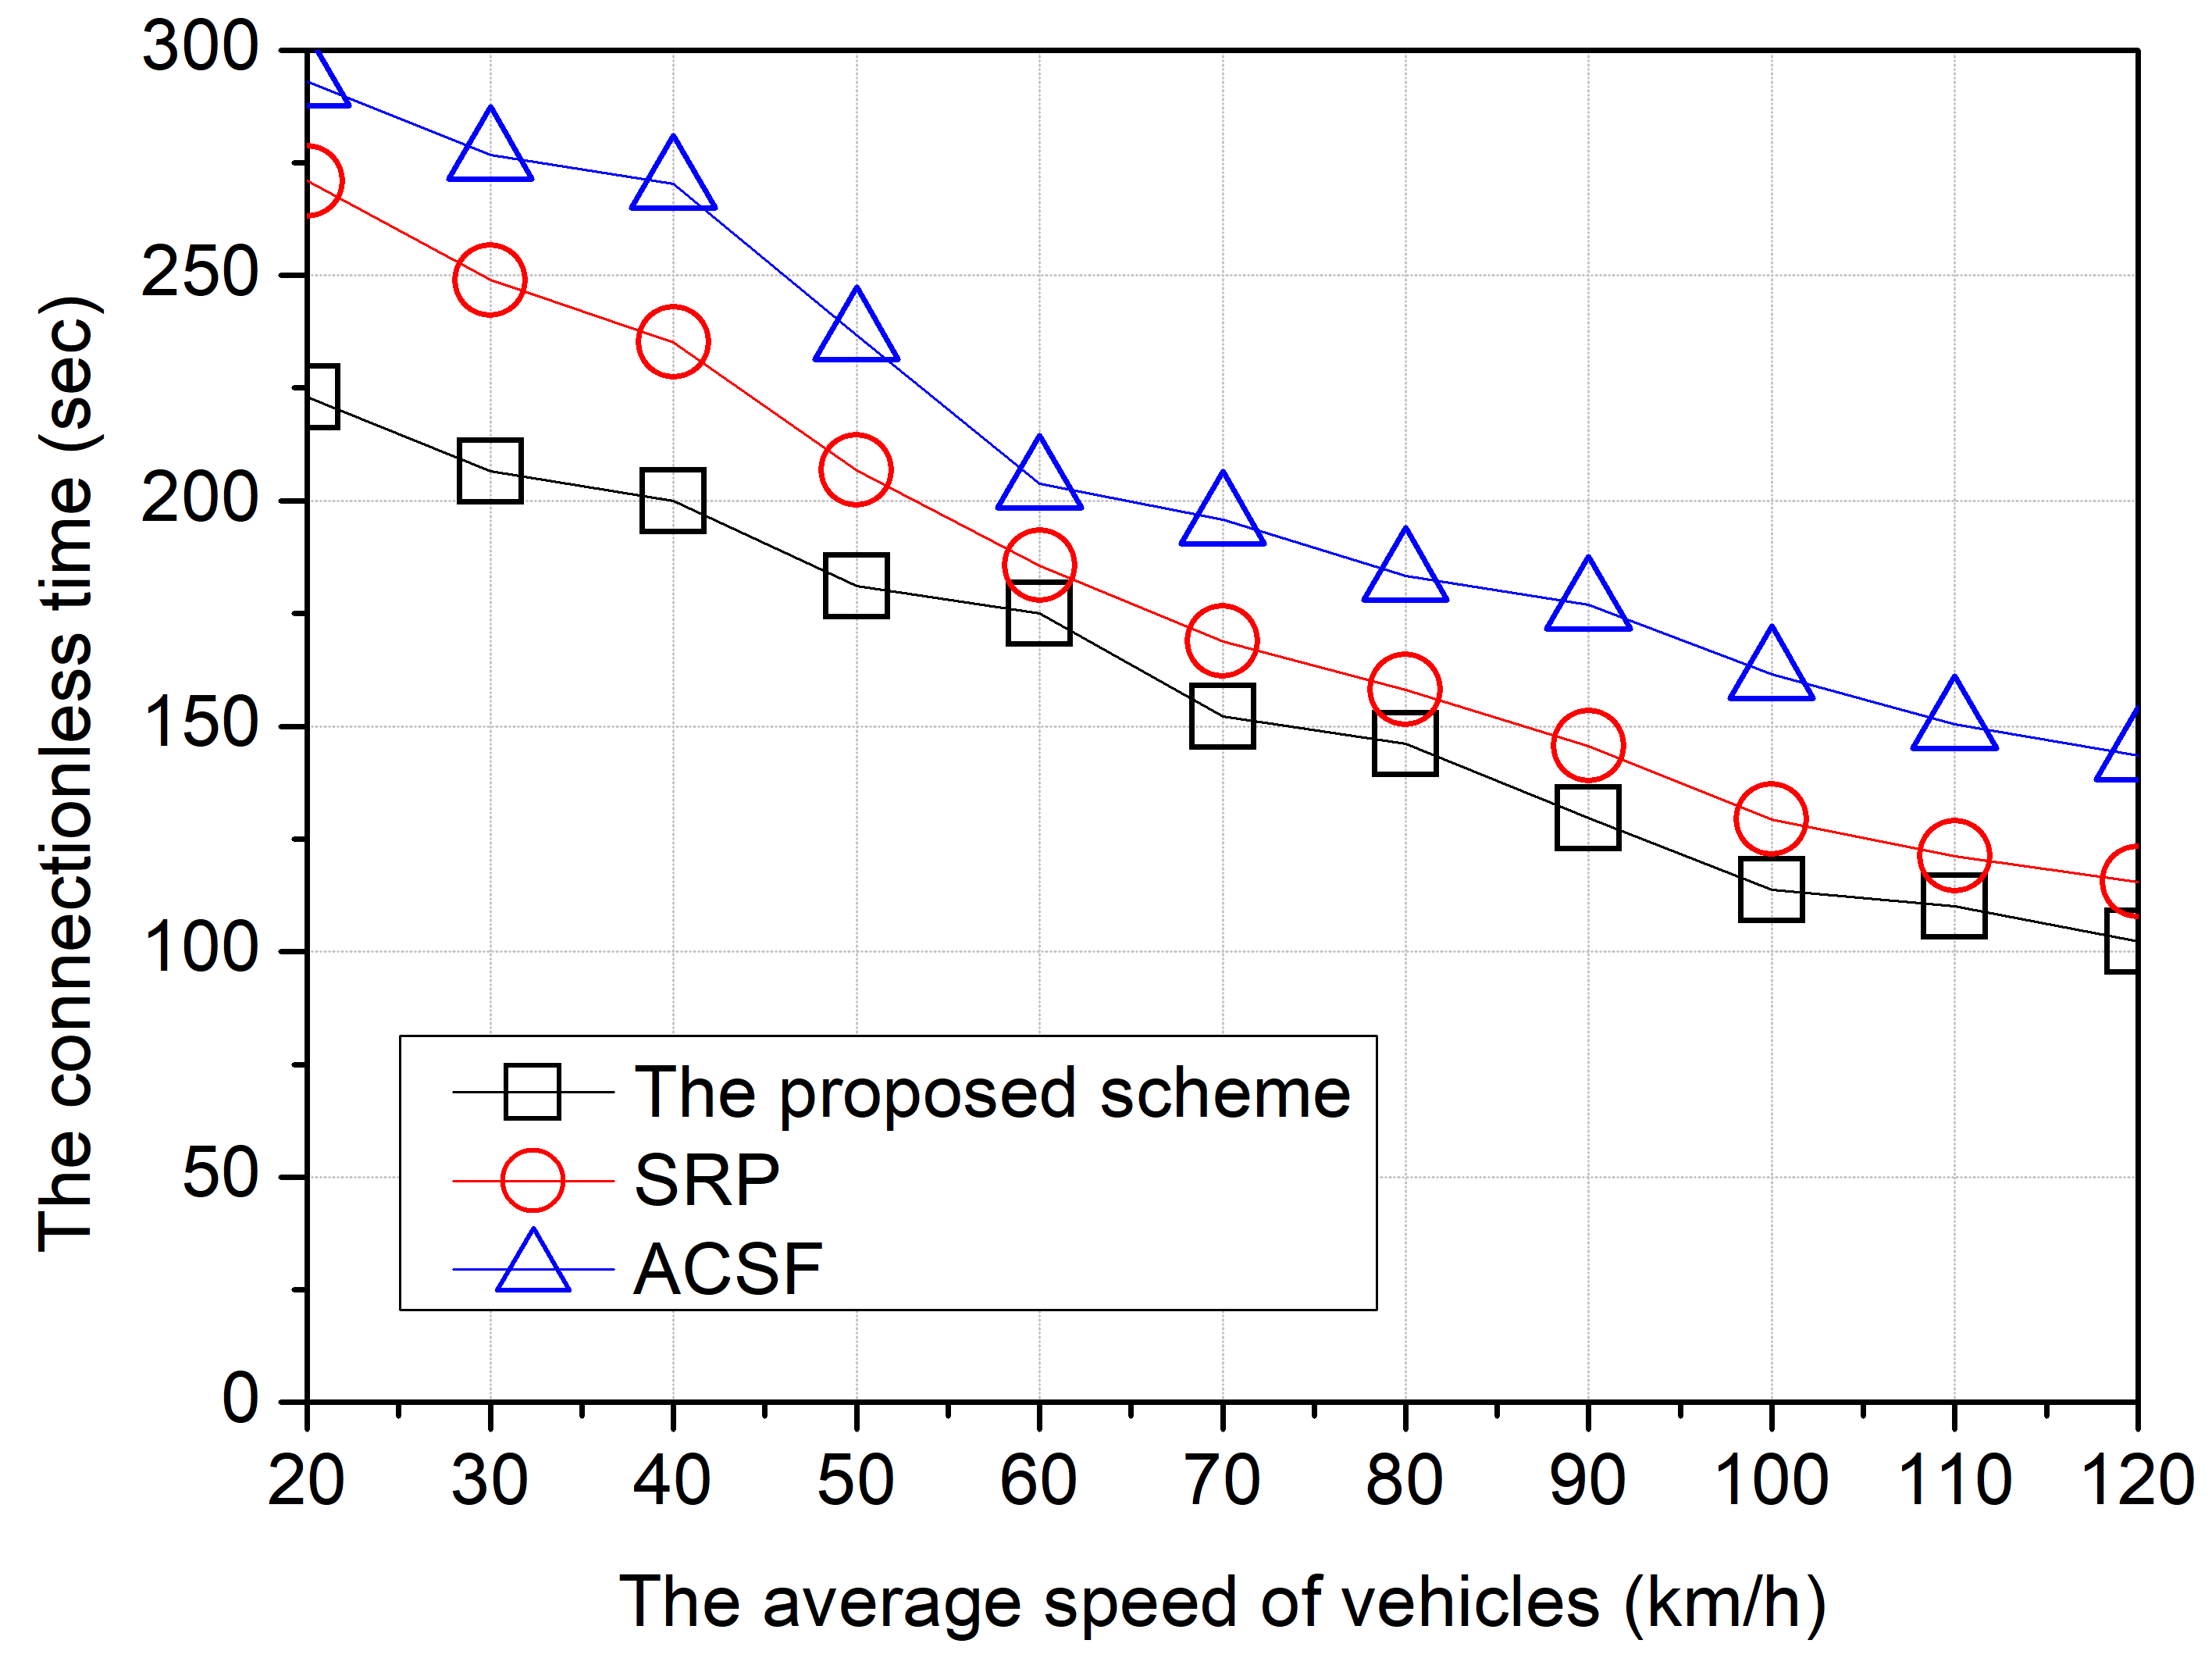
\includegraphics[width=.5\linewidth]{./graphs/VC.png}}
    \caption{The connectionless time according to (\textbf{a}) the data rate; (\textbf{b}) the size of the requested content; (\textbf{c}) the average speed of~vehicles.}
    \label{fig:my_label4}
\end{figure}


\section{Conclusions} \label{sec5}
With the development of self-driving cars, mobile data traffic has surged due to users' demand for content during their free time on the road. This increased traffic leads to delays for users as it burdens the limited wireless communication capacity of base stations (BSs). While roadside units (RSUs) can alleviate this burden, their deployment costs contribute to the existence of outage zones. Existing precaching schemes that utilize one-hop vehicles are unable to minimize these outage zones due to an insufficient number of candidate vehicles. Therefore, we propose a Mobility-based Multi-hop Content Precaching Scheme for Connected and Cooperative Vehicular Networks (CCVNs). We limit the number of hops and the selection of precaching vehicles to minimize overheads and prevent excessive delays from frequent handovers. By~selecting single-hop precaching vehicles, connectionless time is reduced because the requester vehicle can receive the requested content within the outage zone. Additionally, by~selecting multi-hop precaching vehicles, we minimize the dark area time experienced by the requester vehicle. Our simulation results demonstrate that the proposed scheme effectively reduces both connectionless time and dark area time, thereby minimizing the outage zone compared to two representative existing schemes, Adaptive Carry--Store--Forward (ACSF) and Set Ranking-based Precaching (SRP), both based on single-hop~communications.


%\section{Patents}
%This section is not mandatory, but may be added if there are patents resulting from the work reported in this manuscript.
%%%%%%%%%%%%%%%%%%%%%%%%%%%%%%%%%%%%%%%%%%
\vspace{6pt}
%%%%%%%%%%%%%%%%%%%%%%%%%%%%%%%%%%%%%%%%%%
%% optional
%\supplementary{The following supporting information can be downloaded at:  \linksupplementary{s1}, Figure S1: title; Table S1: title; Video S1: title.}

% Only for the journal Methods and Protocols:
% If you wish to submit a video article, please do so with any other supplementary material.
% \supplementary{The following supporting information can be downloaded at: \linksupplementary{s1}, Figure S1: title; Table S1: title; Video S1: title. A supporting video article is available at doi: link.}
%%%%%%%%%%%%%%%%%%%%%%%%%%%%%%%%%%%%%%%%%%
\authorcontributions{Conceptualization, H.C. and Y.N.; methodology, H.C. and Y.N.; software, Y.N. and G.K.; validation, H.C. and G.K.; writing---original draft preparation, H.C. and Y.N.; writing---review and editing, H.C., Y.N. and E.L.; supervision, E.L.; funding acquisition, E.L. All authors have read and agreed to the published version of the~manuscript.}

\funding{This work was supported by a National Research Foundation of Korea (NRF) grant funded by the Korean government (Ministry of Science and ICT (MSIT)) (No. 2022R1A2C1010121).
This work was also supported by funding for the academic research program of Chungbuk National University in~2023.
}
\institutionalreview{Not applicable.}
\informedconsent{Not applicable.}
\dataavailability{Not applicable.} 
\conflictsofinterest{The authors declare no conflicts of~interest.}
%%%%%%%%%%%%%%%%%%%%%%%%%%%%%%%%%%%%%%%%%%
%% Only for journal Encyclopedia
%\entrylink{The Link to this entry published on the encyclopedia platform.}
%%%%%%%%%%%%%%%%%%%%%%%%%%%%%%%%%%%%%%%%%%
%% Optional
\appendixtitles{no} % Leave argument "no" if all appendix headings stay EMPTY (then no dot is printed after "Appendix A"). If~the appendix sections contain a heading then change the argument to~"yes".

%\section[\appendixname~\thesection]{}
%All appendix sections must be cited in the main text. In the appendices, Figures, Tables, etc. should be labeled, starting with ``A''---e.g., Figure A1, Figure A2, etc.
%%%%%%%%%%%%%%%%%%%%%%%%%%%%%%%%%%%%%%%%%%
\begin{adjustwidth}{-\extralength}{0cm}
\reftitle{References} \begin{thebibliography}{999}



\bibitem{Zhe2020} Zhang, Z.; Lung, C.-H.; St-Hilaire, M.; Lambadaris, I. Smart Proactive Caching: Empower the Video Delivery for Autonomous Vehicles in ICN-Based Networks. \textit{IEEE Trans. Veh. Technol.} \textbf{2020}, \emph{69}, 7955--7965.

\bibitem{Shahwani2022} Shahwani, H.; Shah, S.A.; Ashraf, M.; Akram, M.; Jeong, J.; Shin, J. A comprehensive survey on data dissemination in Vehicular Ad~Hoc Networks. \textit{Veh. Commun.} \textbf{2022}, \emph{34}, 100420.

\bibitem{Liu2019} Liu, L.; Zhou, Y.; Yuan, J.; Zhuang, W.; Wang, Y. Economically Optimal MS Association for Multimedia Content Delivery in Cache-Enabled Heterogeneous Cloud Radio Access Networks. \textit{IEEE J. Sel. Areas Commun.} \textbf{2019}, \emph{37}, 1584--1593.

\bibitem{Lee2014} Lee, E.; Lee, E.; Gerla, M.; Oh, S.Y. Vehicular cloud networking: Architecture and design principles. \textit{IEEE Commun. Mag.} \textbf{2014}, \emph{52}, 148--155.

\bibitem{Su2017} Su, Z.; Hui, Y.; Yang, Q. The Next Generation Vehicular Networks: A Content-Centric Framework. \textit{IEEE Wirel. Commun.} \textbf{2017}, \emph{24}, 60--66.

\bibitem{Wang2019} Wang, X.; Wang, X. Vehicular Content-Centric Networking Framework. \textit{IEEE Syst. J.} \textbf{2019}, \emph{13}, 519--529.

\bibitem{Elsayed2022} Elsayed, S.A.; Abdelhamid, S.; Hassanein, H.S. Predictive Proactive Caching in VANETs for Social Networking. \textit{IEEE Trans. Veh. Technol.} \textbf{2022}, \emph{71}, 5298--5313.

\bibitem{AlNagar2022} AlNagar, Y.; Gohary, R.H.; Hosny, S.; El-Sherif, A.A. Mobility-Aware Edge Caching for Minimizing Latency in Vehicular Networks. \textit{IEEE Open J. Veh. Technol.} \textbf{2022}, \emph{3}, 68--84.

\bibitem{Bouk2015C} Bouk, S.H.; Ahmed, S.H.; Kim, D. Vehicular content centric network (VCCN): A survey and research challenges. In Proceedings of the {SAC '15: Proceedings of the 30th Annual ACM Symposium on Applied Computing}, Salamanca, Spain,  13--17 April 2015; pp. 695--700.


\bibitem{Wu2013} Wu, D.; Zhu, G.; Zhao, D. Adaptive Carry-Store Forward Scheme in Two-Hop Vehicular Delay Tolerant Networks. \textit{IEEE Commun. Lett.} \textbf{2013}, \emph{17}, 721--724.

\bibitem{Guo2017} Guo, T.; Li, C.; Miao, Z.; Dong, W.; Su, X. Prefetching-based Content Download for Highway Vehicular Ad~Hoc Networks. In Proceedings of the IEEE International Conference on Communications in China (ICCC), Qingdao, China, 22--24 October 2017.


\bibitem{Wang2017} YWang; Liu, Y.; Zhang, J. Cooperative Store–Carry–Forward Scheme for Intermittently Connected Vehicular Networks. \textit{IEEE Trans. Veh. Technol.} \textbf{2017}, \emph{66}, 777--784.

\bibitem{Park2019} Park, S.; Oh, S.; Nam, Y.; Bang, J.; Lee, E. Mobility-aware Distributed Proactive Caching in Content-Centric Vehicular Networks. In Proceedings of the  {2019 12th IFIP Wireless and Mobile Networking Conference (WMNC)}, Paris, France, 11--13 September 2019; pp. 175--180.

\bibitem{Bang2020} Bang, J.; Nam, Y.; Choi, H.; Lee, E.; Oh, S. Cooperative Content Downloading Protocol Based on the Mobility Information of Vehicles in Intermittently Connected Vehicular Networks. In Proceedings of the  {2020 International Conference on Information Networking (ICOIN)}, Barcelona, Spain, 7--10 January 2020; pp. 273--277.

\bibitem{Wang2021} Wang, R.; Kan, Z.; Cui, Y.; Wu, D.; Zhen, Y. Cooperative Caching Strategy With Content Request Prediction in Internet of Vehicles. \textit{IEEE Internet Things J.} \textbf{2021}, \emph{8}, 8964--8975.

\bibitem{Nam2023} Nam, Y.; Choi, H.; Bang, J.; Shin, Y.; Lee, E. Set Ranking-Based Precaching Protocol in Vehicular Ad~hoc Networks. In Proceedings of the {IEEE Consumer Communications and Networking Conference (CCNC)}, Las Vegas, NV, USA, 8--11 January 2023.

\bibitem{Gupta2000} Gupta, P.; Kumar, P.R. The capacity of wireless networks. \textit{IEEE Trans. Inf. Theory} \textbf{2000}, \emph{46}, 388--404.

\bibitem{Jacobson2009} Jacobson, V.; Smetters, D.K.; Thornton, J.D.; Plass, M.F.; Briggs, N.H.; Braynard, R.L. Networking Named Content. In Proceedings of the {CoNEXT '09: Proceedings of the 5th international conference on Emerging networking experiments and technologies December 2009}, Rome, Italy,  1--4 December 2009; pp. 1--12.

\bibitem{zhang2014} Zhang, L.; Afanasyev, A.; Burke, J.; Jacobson, V.; Claffy, K.; Crowley, P.; Papadopoulos, C.; Wang, L.; Zhang, B. Named data networking. \textit{ACM SIGCOMM Comput. Commun. Rev.} \textbf{2014}, \emph{44}, 66–73.

\bibitem{Amadeo2012} Amadeo, M.; Campolo, C.; Molinaro, A. Content-centric vehicular networking: An evaluation study. In Proceedings of the {Third International Conference on The Network of the Future (NOF)}, Tunis, Tunisia, 21--23 November 2012; pp. 1--5.

\bibitem{Amadeo2012Crown} Amadeo, M.; Campolo, C.; Molinaro, A. CRoWN: Content-Centric Networking in Vehicular Ad~Hoc Networks. \textit{IEEE Commun. Lett.} \textbf{2012}, \emph{16}, 1380--1383.

\bibitem{Salahuddin2014} Salahuddin, M.A.; Al-Fuqaha, A.; Guizani, M.; Cherkaoui, S. RSU cloud and its resource management in support of enhanced vehicular applications. In Proceedings of the {2014 IEEE Globecom Workshops (GC Wkshps)}, Austin, TX, USA, 8--12 December 2014; pp. 127--132.

\bibitem{Rahman2018} Rahman, F.H.; Wan, A.T.; Newaz, S.H.S.; Suhaili, W.S. Vehicular Clustering: Fog Paradigm and Recent Advances. In Proceedings of the {2018 IEEE 18th International Conference on Communication Technology (ICCT)}, Chongqing, China, 8--11 October 2018; pp.~468--472.

\bibitem{Kim2017} Kim, D.; Velasco, Y.; Wang, W.; Uma, R.N.; Hussain, R.; Lee, S. A New Comprehensive RSU Installation Strategy for Cost-Efficient VANET Deployment. \textit{IEEE Trans. Veh. Technol.} \textbf{2017}, \emph{66}, 4200--4211.

\bibitem{Khelifi2020} Khelifi, H.; Luo, S.; Nour, B.; Moungla, H.; Faheem, Y.; Hussain, R.; Ksentini, A. Named Data Networking in Vehicular Ad~Hoc Networks: State-of-the-Art and Challenges. \textit{IEEE Commun. Surv. Tutorials} \textbf{2020}, \emph{22}, 320--351.

\bibitem{Ahmed2018} Ahmed, S.; Mu, D.; Kim, D. Improving Bivious Relay Selection in Vehicular Delay Tolerant Networks. \textit{IEEE Trans. Intell. Transp. Syst.} \textbf{2018}, \emph{19}, 987--995.

\bibitem{Bouk2015J} Bouk, S.; Ahmed, S.; Omoniwa, B.; Kim, D. Outage Minimization Using Bivious Relaying Scheme in Vehicular Delay Tolerant Networks. \textit{Wirel. Pers. Commun.} \textbf{2015}, \emph{84}, 2679–2692.

\bibitem{Chen2009} Chen, B.; Chan, M. MobTorrent: A Framework for Mobile Internet Access from Vehicles. In Proceedings of the {IEEE INFOCOM}, Rio de Janeiro, Brazil, 19--25 April 2009.

\bibitem{Wave} Paier, A.; Tresch, R.; Alonso, A.; Smely, D.; Meckel, P.; Zhou, Y.; Czink, N. Average Downstream Performance of Measured IEEE 802.11p Infrastructure-to-Vehicle Links. In Proceedings of the {2010 IEEE International Conference on Communications Workshops}, Cape Town, South Africa, 23--27 May 2010; pp. 1--5.

\bibitem{Suthaputchakun2018} Suthaputchakun, C.; Sun, Z.  Multihop Broadcast Protocol in Intermittently Connected Vehicular Networks. \textit{IEEE Trans. Aerosp. Electron. Syst.} \textbf{2018}, \emph{54}, 616--628.

\bibitem{Wu2020} Wu, J.; Guo, Y.; Zhou, H.; Shen, L.; Liu, L. Vehicular Delay Tolerant Network Routing Algorithm Based on Bayesian Network. \textit{IEEE Access} \textbf{2020}, \emph{8}, 18727--18740.

\bibitem{Peyman2023} Peyman, M.; Fluechter, T.; Panadero, J.; Serrat, C.; Xhafa, F.; Juan, A. Optimization of Vehicular Networks in Smart Cities: From Agile Optimization to Learnheuristics and Simheuristics. \textit{Sensors} \textbf{2023}, \emph{23}, 499.

\bibitem{NS3}Network Simulator 3 (NS3). Available online: \url{https://www.nsnam.org}~(accessed on 10 September 2024).



\end{thebibliography}
\PublishersNote{}
\end{adjustwidth}
\end{document}